% ----------------------------------------------
% abnTeX2: Modelo de Trabalho Academico (tese de doutorado, dissertacao de mestrado e trabalhos monograficos em geral) em conformidade com ABNT NBR 14724:2011: Informacao e documentacao - Trabalhos academicos - Apresentacao
% ----------------------------------------------

% ==============================================
% ||||||||||||||||||||||||||||||||||||||||||||||
% ----------------------------------------------

\documentclass[
	% -- opções da classe memoir --
	12pt,		% tamanho da fonte
	%openright,	% capítulos começam em pág ímpar (insere página vazia caso preciso)
	oneside,	% para impressão em verso e anverso. Oposto a oneside
	a4paper,	% tamanho do papel. 
	% -- opções da classe abntex2 --
	chapter=TITLE,		% títulos de capítulos convertidos em letras maiúsculas
	%section=TITLE,		% títulos de seções convertidos em letras maiúsculas
	%subsection=TITLE,	% títulos de subseções convertidos em letras maiúsculas
	%subsubsection=TITLE,% títulos de subsubseções convertidos em letras maiúsculas
	% -- opções do pacote babel --
	english,	% idioma adicional para hifenização
%	french,		% idioma adicional para hifenização - problemas com circuitikz
%	spanish,	% idioma adicional para hifenização
	brazil		% o último idioma é o principal do documento
	]{abntex2}

% ----------------------------------------------
% Pacotes de fontes... 
% ----------------------------------------------
\usepackage[utf8]{inputenc}	% Codificacao do documento (conversão automática dos acentos)
\usepackage[T1]{fontenc}	% Selecao de codigos de fonte. Afeta separação de sílabas
\usepackage{lmodern}	% Usa a fonte Latin Modern
\renewcommand{\ABNTEXchapterfont}{\fontfamily{ptm}\fontseries{sbc}\selectfont} % Familia de fontes times
%\usepackage{times}		% Usa a fonte Times
%\usepackage{palatino}	% Usa a fonte Palatino
%\usepackage{mathpazo}	% Usa a fonte Adobe Palatino
%\usepackage[scaled=.92]{helvet}	% Usa a fonte Helvetica
\usepackage{mathptmx}	% para utilização de times

% ----------------------------------------------
% Configuração das fontes
% ----------------------------------------------
% Algumas configurações de fontes para capitulos e seções tanto no texto quanto no sumário
\renewcommand{\ABNTEXchapterfont}{\bfseries}
\renewcommand{\ABNTEXchapterfontsize}{\Large}
\renewcommand{\ABNTEXpartfont}{\ABNTEXchapterfont}
\renewcommand{\ABNTEXpartfontsize}{\ABNTEXchapterfontsize}
\renewcommand{\cftpartfont}{\normalfont\bfseries}
\renewcommand{\ABNTEXsectionfont}{\bfseries}
\renewcommand{\ABNTEXsectionfontsize}{\large}
\renewcommand{\ABNTEXsubsectionfont}{\normalfont}
\renewcommand{\ABNTEXsubsectionfontsize}{\normalsize}
\renewcommand{\cftsubsectionfont}{\normalfont}
\renewcommand{\ABNTEXsubsubsectionfont}{\slshape}
\renewcommand{\cftsubsubsectionfont}{\normalfont\slshape}
\renewcommand{\ABNTEXsubsubsubsectionfont}{\bfseries}
\renewcommand{\ABNTEXsubsectionfont}{\bfseries}

% Para configurar mais níveis configure conforme utilizado acima e comente as duas linhas abaixo
\settocdepth{subsubsection} % configura sumário para apresentar subseções até o quarto nível
\setsecnumdepth{subsubsection} % configura para numerar subseções até o quarto nível. Subseções de quinto nível não conterão numeração.

\addto\captionsbrazil{\renewcommand{\listfigurename}{Lista de figuras}} % Altera nome da lista de ilustrações para lista de figuras

\addto{\captionsbrazil}{\renewcommand{\bibname}{Refer\^encias Bibliogr\'aficas}} % Altera nome Referencias para Referencias Bibliogarficas

% ----------------------------------------------
% Para criar Quadros - ABNT 14724 5.10
% ----------------------------------------------
\newcommand{\quadroname}{Quadro}
\newcommand{\listofquadrosname}{Lista de quadros}
\newfloat[chapter]{quadro}{loq}{\quadroname}
\newlistof{listofquadros}{loq}{\listofquadrosname}
\newlistentry{quadro}{loq}{0}
\counterwithout{quadro}{chapter}
\renewcommand{\cftquadroname}{\quadroname\space}
\renewcommand*{\cftquadroaftersnum}{\hfill--\hfill}

% ----------------------------------------------
% Para criar Gráficos
% ----------------------------------------------
\newcommand{\graficoname}{Gráfico}
\newcommand{\listofgraficosname}{Lista de gráficos}
\newfloat[chapter]{grafico}{logf}{\graficoname}
\newlistof{listofgraficos}{logf}{\listofgraficosname}
\newlistentry{grafico}{logf}{0}
\counterwithout{grafico}{chapter}
\renewcommand{\cftgraficoname}{\graficoname\space}
\renewcommand*{\cftgraficoaftersnum}{\hfill--\hfill}

% ----------------------------------------------
% Equações com numeração sequencial
% ----------------------------------------------
\counterwithout{equation}{chapter}

% ----------------------------------------------
% Pacotes básicos 
% ----------------------------------------------
\usepackage{lastpage}		% Usado pela ficha catalografica
\usepackage{indentfirst}	% Indenta o primeiro paragrafo de cada seção.
\usepackage{color}			% Controle das cores
\usepackage{graphicx}		% Inclusão de gráficos
\usepackage{microtype} 		% para melhorias de justificação
\usepackage{array}
%\usepackage{gensymb}       % Símbolos

\usepackage{amsmath} 	%--------------------------%
\usepackage{hyperref} 	%--------------------------%
\usepackage{bibentry} 	% para inserir refs. bib. no meio do texto


% ----------------------------------------------
% Pacotes adicionais
% ----------------------------------------------
\usepackage{lipsum}				% para geração de dummy text
\usepackage[colorinlistoftodos, english]{todonotes}
% uso: \todo[inline, color=red!80]{texto}
\usepackage{verbatim}
\usepackage{soulutf8}
% uso: \hl{highlight} ou \st{strikeout} ou \ul{underline}
%\usepackage{tabularx}
\usepackage{rotating,tabularx}
\usepackage{multirow}
\usepackage{multicol}
\usepackage{lscape}
\usepackage{varwidth}
\usepackage{subfig}
\usepackage{pdfpages}
\usepackage{pgfplots}
\pgfplotsset{compat=1.12}
\usepackage{float}
\usepackage[nohyperlinks]{acronym}
%\usepackage{subfigure}

% Para desenho de circuitos
\usepackage{tikz}
\usepackage[american]{circuitikz}
\usepackage{siunitx}
\usepackage{colortbl}

%para usar codeblock
\usepackage{listings}
\definecolor{dkgreen}{rgb}{0,0.6,0}
\definecolor{gray}{rgb}{0.5,0.5,0.5}
\definecolor{mauve}{rgb}{0.58,0,0.82}
\lstset{frame=tb,
  language=C,
  aboveskip=3mm,
  belowskip=3mm,
  showstringspaces=false,
  columns=flexible,
  basicstyle={\small\ttfamily},
  numbers=left,
  numberstyle=\tiny\color{gray},
  keywordstyle=\color{blue},
  commentstyle=\color{dkgreen},
  stringstyle=\color{mauve},
  breaklines=true,
  breakatwhitespace=true,
  tabsize=3
} 

\usepackage{booktabs}
\usepackage{adjustbox}
\usepackage{placeins}
\usepackage{longtable}
\usepackage{caption}
\usepackage{amssymb}

% ----------------------------------------------
% Pacotes de citações
% ----------------------------------------------
\usepackage[brazilian,hyperpageref]{backref}	 % Paginas com as citações na bibl
\usepackage[alf]{abntex2cite}	% Citações padrão ABNT

% ==============================================
% CONFIGURAÇÕES DE PACOTES
% ==============================================

\DeclareCaptionFormat{caption_with_break_line}{%
  % #1: label (e.g. "Table 1")
  % #2: separator (e.g. ": ")
  % #3: caption text
  \begin{varwidth}{\linewidth}%
    \centering
    #1#2#3%
  \end{varwidth}%
}

% ----------------------------------------------
% Configurações do pacote backref 
% usado sem a opção hyperpageref de backref
% ----------------------------------------------
\renewcommand{\backrefpagesname}{Citado na(s) página(s):~}
% Texto padrão antes do número das páginas
\renewcommand{\backref}{}
% Define os textos da citação
\renewcommand*{\backrefalt}[4]{
	\ifcase #1 %
		Nenhuma citação no texto.%
	\or
		Citado na página #2.%
	\else
		Citado #1 vezes nas páginas #2.%
	\fi}%

% ----------------------------------------------
% Espaçamentos entre linhas e parágrafos 
% ----------------------------------------------
% O tamanho do parágrafo é dado por:
\setlength{\parindent}{1.3cm}

% Controle do espaçamento entre um parágrafo e outro:
\setlength{\parskip}{0.2cm}  % tente também \onelineskip

% impedir quebra de notas de rodapé entre páginas
\interfootnotelinepenalty=10000

% ----------------------------------------------
% compila o indice
% ----------------------------------------------
\makeindex

% ||||||||||||||||||||||||||||||||||||||||||||||
% Informações de dados para CAPA e FOLHA DE ROSTO
% ||||||||||||||||||||||||||||||||||||||||||||||
\titulo{EDUCAÇÃO FINANCEIRA NO ENSINO MÉDIO INTEGRADO DOS INSTITUTOS FEDERAIS: UMA PROPOSTA ASSISTIDA POR JOGOS COMO TECNOLOGIA EDUCACIONAL} % Não utilize o ponto final no título
\autor{Johnata Souza Santicioli}
\local{Porto Alegre}
\data{2020}
\orientador{Prof. Dr. Evandro Manara Miletto}
\coorientador{Profa. Dra. Josiane Carolina S. R. Procasko} % comente esta linha caso nao tenha coorientador
\instituicao{%
  INSTITUTO FEDERAL DO RIO GRANDE DO SUL
  \par
  CAMPUS PORTO ALEGRE
  \par
  PROGRAMA DE MESTRADO PROFISSIONAL EM 
  \par
  INFORMÁTICA NA EDUCAÇÃO
  } 
\tipotrabalho{Dissertação (Mestrado)}
% O preambulo deve conter o tipo do trabalho, o objetivo, 
% o nome da instituição e a área de concentração 

%Preâmbulo da Qualificação
\preambulo{Proposta de Dissertação apresentada junto ao Programa de Pós-graduação Stricto Sensu – Mestrado Profissional em Informática na Educação do Instituto Federal de Educação, Ciência e Tecnologia do Rio Grande do Sul – Campus Porto Alegre, como requisito parcial ao desenvolvimento da Dissertação.}

%Preâmbulo da Dissertação
%\preambulo{Dissertação apresentada ao Programa de Pós-graduação Stricto Sensu – Mestrado Profissional em Informática na Educação do Instituto Federal de Educação, Ciência e Tecnologia do Rio Grande do Sul – Campus Porto Alegre, como parte dos requisitos para obtenção do título de Mestre em Informática na Educação.}

%\preambulo{Trabalho apresentado como requisito para a obtenção do título de Mestre, pelo Programa de Pós-Graduação em Engenharia Elétrica do Instituto Federal de Educação, Ciência e Tecnologia do Rio Grande do Sul – Campus Porto Alegre.}

% ----------------------------------------------
% Configurações de aparência do PDF final
% ----------------------------------------------
% alterando o aspecto da cor azul
\definecolor{blue}{RGB}{41,5,195}

% alterando o aspecto da cor cinza
\definecolor{gray}{RGB}{50,50,50}

% informações do PDF
\makeatletter
\hypersetup{
     	%pagebackref=true,
		pdftitle={\imprimirtitulo}, 
		pdfauthor={\imprimirautor},
    	pdfsubject={\imprimirpreambulo},
	    pdfcreator={LaTeX - abnTeX2 - Overleaf},
        pdfkeywords={abnt}{latex}{abntex2}{trabalho acadêmico}{ifsul}{mpie}{mestrado profissional}, 
		colorlinks=true, % false: boxed links; true: colored links
    	linkcolor=black, % color of internal links
    	citecolor=black, % color of links to bibliography
    	filecolor=blue,  % color of file links
		urlcolor=gray,	 % color of url links
		bookmarksdepth=4
}
\makeatother

\begin{document}
% Seleciona o idioma do documento (conforme pacotes do babel)
%\selectlanguage{english}
\selectlanguage{brazil}

% Retira espaço extra obsoleto entre as frases.
\frenchspacing 

\newpage

% ==============================================
% ELEMENTOS PRÉ-TEXTUAIS
% ==============================================
\pretextual

% ----------------------------------------------
% Capa
% ----------------------------------------------
%\imprimircapa
% Capa personalizada sem o uso de \imprimircapa
\begin{capa} 
   \center
   \ABNTEXchapterfont\large\bfseries{\imprimirinstituicao} 
   \vfill
   %\vspace*{1cm}
   \ABNTEXchapterfont\large\bfseries\textsc{\MakeUppercase{\imprimirautor}}
   \vfill
   \begin{center}
   \ABNTEXchapterfont\Large\bfseries{\MakeUppercase{\imprimirtitulo}}
   \end{center}
   \vfill
   \vspace*{5cm}
   \large\bfseries\MakeTextUppercase{\imprimirlocal} \\
   \large\bfseries\imprimirdata
   \vspace*{1cm}
\end{capa}

% ----------------------------------------------
% Folha de rosto
% ----------------------------------------------
% folha de rosto personalizada sem uso de \imprimirfolhaderosto
\makeatletter
\renewcommand{\folhaderostocontent}{
\begin{center}
  {\ABNTEXchapterfont\large\imprimirautor}
  \vspace*{\fill}%\vspace*{\fill}
  \begin{center}
  \ABNTEXchapterfont\bfseries\Large\imprimirtitulo
  \end{center}
  \vspace*{\fill}
  
  \abntex@ifnotempty{\imprimirpreambulo}{%
    % \hspace{.45\textwidth}
    % \begin{minipage}{.5\textwidth}
    \hspace{.39\textwidth}
    \begin{minipage}{.6\textwidth}
        \SingleSpacing
        \imprimirpreambulo
    \end{minipage}%
    \vspace*{\fill}
  }%
  
  \abntex@ifnotempty{\imprimirorientador}{%
%   \hspace{.45\textwidth}
%   \begin{minipage}{.5\textwidth}
    \hspace{.39\textwidth}
    \begin{minipage}{.6\textwidth}
	    {\imprimirorientadorRotulo~\newline Profº. Dr. \imprimirorientador}%
    \end{minipage}%
  }%
  
  \vspace*{.005\textwidth}
  
  \abntex@ifnotempty{\imprimircoorientador}{%
%   \hspace{.45\textwidth}
%   \begin{minipage}{.5\textwidth}
    \hspace{.39\textwidth}
    \begin{minipage}{.6\textwidth}
    {\imprimircoorientadorRotulo~\newline Profª. Dra. \imprimircoorientador}%
  \end{minipage}%
  }%
  
  \vspace*{\fill}
  %{\abntex@ifnotempty{\imprimirinstituicao}{\imprimirinstituicao\vspace*{\fill}}}

  {\large\imprimirlocal}
  \par
  {\large\imprimirdata}
  \vspace*{1cm}
\end{center}
}
\makeatother

% Folha de rosto (o * indica que haverá a ficha bibliográfica)
\imprimirfolhaderosto*

% ----------------------------------------------
% Inserir a ficha bibliografica catalográfica
% ----------------------------------------------
% Isto é um exemplo de Ficha Catalográfica, ou ``Dados internacionais de catalogação-na-publicação''. Você pode utilizar este modelo como referência. Porem, provavelmente a biblioteca da sua universidade lhe fornecerá um PDF com a ficha catalográfica definitiva após a defesa do trabalho. Quando estiver com o documento, salve-o como PDF no diretório do seu projeto e substitua todo o conteúdo de implementação deste arquivo pelo comando abaixo:

% \begin{fichacatalografica}
%     \includepdf{fig_ficha_catalografica.pdf}
% \end{fichacatalografica}
\begin{fichacatalografica}
	\sffamily
	\vspace*{\fill}					% Posição vertical
  	\begin{center}					% Minipage Centralizado
    	\fbox{
            \begin{minipage}[t]{1,5cm} 
                \vspace{0.5cm} 
                S358j %Algum número que o bibliotecário ira gerar
            \end{minipage}
            
            \begin{minipage}[t]{11cm}	% Largura
            	\small
                \vspace{0.5cm}
            	%\imprimirautor		% ATENCAO - SUBSTITUIR POR %Sobrenome, Nome do autor
                Santicioli, Johnata Souza
            	
            	\hspace{0.5cm} 
                \imprimirtitulo  / \imprimirautor; orientador:  \imprimirorientador; coorientadora: \imprimircoorientador. -- \imprimirlocal: \imprimirdata.\\
            	
            	\hspace{0.5cm}
                \pageref{LastPage} f.\\ % : il. (algumas color.) 
                % ; 30 cm.\\
                
            	
                \hspace{0.5cm}
            	\imprimirtipotrabalho~--~Instituto Federal do Rio Grande do Sul -- Campus Porto Alegre. Programa de Metrado Profissional em Informática na Educação, \imprimirlocal, \imprimirdata. \imprimirorientadorRotulo~Profº. Dr. \imprimirorientador ;
                \imprimircoorientadorRotulo~Profª. Dra. \imprimircoorientador.\\
            	
            	\hspace{0.5cm}
            		1. Alfabetização e Educação Financeira
            		2. Ensino Médio Integrado
            		3. Institutos Federais do Brasil
            		4. Jogos Sérios
            		5. Epistemologia Genética Piagetiana
            		I. Miletto, Evandro Manara.
                    II. Procasko, Josiane Carolina Soares Ramos.
                    III. Título.\\
                
            	\hspace{8.75cm} CDU 621.3 %algum outro numero
            \end{minipage}
        }
        \hspace{0.5cm}
        Dados Internacionais de Catalogação na Publicação (CIP) \\  	
        (Bibliotecário: Nome Sobrenome – CRB 10/1298)
    \end{center}
\end{fichacatalografica}

% ----------------------------------------------
% Inserir errata
% ----------------------------------------------
% \begin{errata}
% Elemento opcional da \citeonline[4.2.1.2]{NBR14724:2011}. Exemplo:

% \vspace{\onelineskip}

% FERRIGNO, C. R. A. \textbf{Tratamento de neoplasias ósseas apendiculares com reimplantação de enxerto ósseo autólogo autoclavado associado ao plasma rico em plaquetas}: estudo crítico na cirurgia de preservação de membro em cães. 2011. 128 f. Tese (Livre-Docência) - Faculdade de Medicina Veterinária e Zootecnia, Universidade de São Paulo, São Paulo, 2011.

% \begin{table}[htb]
% \center
% \footnotesize
% \begin{tabular}{|p{1.4cm}|p{1cm}|p{3cm}|p{3cm}|}
%   \hline
%    \textbf{Folha} & \textbf{Linha}  & \textbf{Onde se lê}  & \textbf{Leia-se}  \\
%     \hline
%     1 & 10 & auto-conclavo & autoconclavo\\
%    \hline
% \end{tabular}
% \end{table}

% \end{errata}

%\endinput

% ----------------------------------------------
% Inserir folha de aprovação
% ----------------------------------------------
% Isto é um exemplo de Folha de aprovação, elemento obrigatório da NBR 14724/2011 (seção 4.2.1.3). Você pode utilizar este modelo até a aprovação do trabalho. Após isso, substitua todo o conteúdo deste arquivo por uma imagem da página assinada pela banca com o comando abaixo:
%
% \includepdf{folhadeaprovacao_final.pdf}
%
%\begin{folhadeaprovacao}
% Gerada conforme instrucoes do PPGEE
%  \begin{center}
%  {\ABNTEXchapterfont\large\imprimirautor}

%  \vspace*{\fill}\vspace*{\fill}
%    \begin{center}
%    	\ABNTEXchapterfont\bfseries\Large\imprimirtitulo
%    \end{center}
%  \vspace*{\fill}

%  \hspace{.45\textwidth}
%    \begin{minipage}{.5\textwidth}
%    	\imprimirpreambulo 
%    \end{minipage}%

%  \vspace*{\fill}
%    \begin{flushleft}
%  	  Aprovado em 20 de Dezembro de 2017. \\
%    \end{flushleft}
%  \vspace*{\fill}
%    BANCA EXAMINADORA:% \imprimirlocal, \today :
%  \end{center}
   
   %\assinatura{\textbf{\imprimirorientador} \\ Orientador}
   %\assinatura{\textbf{\imprimircoorientador} \\ coorientador} 
   
%   \assinatura{Prof. Dr. Nome Sobrenome -- Unisinos \\ Avaliador}
%   \assinatura{Prof. Dr. Nome Sobrenome -- UFRGS \\ Avaliador Externo}
%   \assinatura{Prof. Dr. Nome Sobrenome -- UERGS \\ Avaliador Externo}
   %\assinatura{\textbf{Professor} \\ Convidado 4}
     
 %   \vspace*{\fill} \vspace*{\fill}
 %   \hspace{.4\textwidth}
 %   \begin{minipage}{.5\textwidth}
 %   	\imprimirorientador~(Orientador) \\
 %       \imprimircoorientador~(coorientador)
 %   \end{minipage}%
    
%    \vspace*{\fill}
%    \begin{flushleft}
%    	Visto e permitida a impressão\\
%        \imprimirlocal
%    \end{flushleft}
    
%    \vspace*{\fill}
%    \hspace{.4\textwidth}
%    \begin{minipage}{.5\textwidth}
%    	Profa. Dra. Silvia de Castro Bertagnolli \\
%        Coordenador Mestrado Profissional em Informática na Educação
%    \end{minipage}
%    \begin{center}
%     \vspace*{0.5cm}
%       {\large\imprimirlocal}
%       \par
%       {\large\imprimirdata}
%       \vspace*{1cm}
%   \end{center}
  
%\end{folhadeaprovacao}

% ----------------------------------------------
% Dedicatória
% ----------------------------------------------
% \newpage
% \begin{dedicatoria}
%   \vspace*{\fill}
%   \centering
%   \noindent
%   \textit{A principal meta da educação é criar homens que sejam capazes de fazer coisas novas, não simplesmente repetir o que outras gerações já fizeram. Homens que sejam criadores, inventores, descobridores. A segunda meta da educação é formar mentes que estejam em condições de criticar, verificar e não aceitar tudo que a elas se propõe.\\
%   (Jean Piaget)} 
%   \vspace*{\fill}
% \end{dedicatoria}

% ----------------------------------------------
% Agradecimentos
% ----------------------------------------------
%\begin{agradecimentos}

%    \lipsum[1]
%\end{agradecimentos}

% ----------------------------------------------
% Epígrafe
% ----------------------------------------------
% Importante: O autor da epígrafe deve constar na lista de referências
\newpage
\begin{epigrafe}
    \vspace*{\fill}
	\begin{flushright}
		\textit{Seria uma atitude ingênua esperar que as classes dominantes desenvolvessem uma forma de educação que proporcionasse às classes dominadas perceber as injustiças sociais de maneira crítica.\\
        (Paulo Freire)}
    \end{flushright}
    \begin{flushright}
        \textit{Por que gastais o dinheiro naquilo que não é pão? E o produto do vosso trabalho naquilo que não pode satisfazer? Ouvi-me atentamente, e comei o que é bom, e a vossa alma se deleite com a gordura.\\
        (Isaías 55.2)}
	\end{flushright}
\end{epigrafe}

% ||||||||||||||||||||||||||||||||||||||||||||||
% RESUMOS
% ||||||||||||||||||||||||||||||||||||||||||||||

% ----------------------------------------------
% Resumo em português
% ----------------------------------------------
% Importante: De acordo com a NBR6024 as palavras-chaves devem ser separadas entre si por ponto e devem ter somente a primeira palavra escrita com letra maiúscula
\setlength{\absparsep}{18pt} % ajusta o espaçamento dos parágrafos do resumo
\begin{resumo}
	Uma parcela dos consumidores brasileiros estão endividados excessivamente, inadimplentes ou com restrição ao crédito, esse número tende a aumentar por conta da crise financeira e de saúde causada pela pandemia do COVID-19. Ademais, os jovens adolescentes brasileiros possuem um baixo índice de letramento financeiro, em comparação a outros países que participaram do estudo publicado pela Organização para a Cooperação e Desenvolvimento Econômico. Sem considerar os problemas com pobreza e distribuição de renda do país, esse contexto evidencia o reflexo do baixo letramento e conhecimento financeiro da população brasileira. A inserção desse tema nos currículos acadêmicos representa um grande desafio para as instituições de ensino da Rede Federal de Educação Profissional, Científica e Tecnológica (RFEPCT), em especial, que tem como missão a formação profissional, cidadã e conectada ao mundo contemporâneo. Nesse contexto, o presente projeto tem o objetivo avaliar a efetividade de um curso sobre educação financeira assistido por jogos sérios, como tecnologia educacional principal, para prover educação financeira aos estudantes do ensino médio. A metodologia utilizada no curso é embasada nos estágios do desenvolvimento cognitivo do letramento financeiro, elaborada com apoio da epistemologia genética de Jean Piaget. O processo implica o uso dos jogos Orçamento Consciente e Renda Passiva para simular ambientes, simplificar e apresentar de forma lúdica os temas fundamentais sobre a educação financeira. A presente pesquisa é classificada como aplicada quanto à sua natureza, exploratória quanto aos objetivos e de estudo de caso quanto à sua finalidade e procedimentos, os dados foram coletados por meio de questionários e analisados através da abordagem qualitativa. No intuito de validar a presente pesquisa o curso “Educação Financeira através de Jogos” foi ofertado aos alunos do ensino médio integrado no Instituto Federal Sul-rio-grandense (IFSUL) - Câmpus Gravataí, por intermédio de um projeto de ensino aprovado pela pró-reitoria de ensino da instituição. Os resultados da pesquisa, confirmaram a hipótese que os jogos utilizados favoreceram a aprendizagem dos estudantes, bem como comprovaram que o curso proporcionou aos alunos conhecimentos introdutórios sobre finanças e atendeu as expectativas dos participantes e dos pesquisadores, desta forma ele pode ser expandido para outras unidades de ensino para diminuir essa importante lacuna educacional.
% 	\vspace{\onelineskip}
	
 	\noindent 
	\textbf{Palavras-chaves}: Alfabetização e Educação Financeira; Ensino Médio Integrado; Institutos Federais do Brasil; Jogos Sérios; Epistemologia Genética Piagetiana.
\end{resumo}

% ----------------------------------------------
% Resumo em inglês
% ----------------------------------------------
% Importante: De acordo com a NBR6024 as palavras-chaves devem ser separadas entre si por ponto e devem ter somente a primeira palavra escrita com letra maiúscula
\begin{resumo}[Abstract]
\begin{otherlanguage*}{english}

O resumo em inglês será construído a partir do resumo final do trabalho.    
% 	\vspace{\onelineskip}
 
	\noindent 
	\textbf{Keywords}: Literacy and Financial Education; Integrated High School; Federal Institutes of Brazil; Serious Games; Piagetian Genetic Epistemology.
\end{otherlanguage*}
\end{resumo}

% ----------------------------------------------
% resumo em francês 
% ----------------------------------------------
% Importante: De acordo com a NBR6024 as palavras-chaves devem ser separadas entre si por ponto e devem ter somente a primeira palavra escrita com letra maiúscula
% \begin{resumo}[Résumé]
%  \begin{otherlanguage*}{french}
%     Il s'agit d'un résumé en français.
 
%    \textbf{Mots-clés}: latex. abntex. publication de textes.
%  \end{otherlanguage*}
% \end{resumo}

% ----------------------------------------------
% resumo em espanhol
% ----------------------------------------------
% Importante: De acordo com a NBR6024 as palavras-chaves devem ser separadas entre si por ponto e devem ter somente a primeira palavra escrita com letra maiúscula
% \begin{resumo}[Resumen]
%  \begin{otherlanguage*}{spanish}
%    Este es el resumen en español.
  
%    \textbf{Palabras clave}: latex. abntex. publicación de textos.
%  \end{otherlanguage*}
 
% \end{resumo}

% ----------------------------------------------
% inserir lista de ilustrações (ou figuras)
% ----------------------------------------------
\pdfbookmark[0]{\listfigurename}{lof}
\listoffigures*
\cleardoublepage

% Diferentes tipos de listas podem ser criadas por meio de macros do memoir.

% ----------------------------------------------
% inserir lista de tabelas
% ----------------------------------------------
\pdfbookmark[0]{\listtablename}{lot}
\listoftables*
\cleardoublepage

% ----------------------------------------------
% inserir lista de quadros (ex.: \begin{quadro} \end{quadro})
% ----------------------------------------------
\pdfbookmark[0]{\listofquadrosname}{loq}
\listofquadros*
\cleardoublepage

% ----------------------------------------------
% inserir lista de Graficos (ex.: \begin{grafico} \end{grafico})
% ----------------------------------------------
\pdfbookmark[0]{\listofgraficosname}{logf}
\listofgraficos*
\cleardoublepage

% ----------------------------------------------
% inserir lista de abreviaturas e siglas
% ----------------------------------------------
% Importante: As abreviaturas e siglas devem estar em ordem alfabética
%\begin{siglas}
%  \item[ABNT] Associação Brasileira de Normas Técnicas
%  \item[abnTeX] ABsurdas Normas para TeX
%
\begin{siglas}
    \item[\textbf{AEF}] Associação de Educação Financeira
    \item[\textbf{ANBIMA}] Associação Brasileira das Entidades dos Mercados Financeiros e de Capitais
    \item[\textbf{B3}] Brasil, Bolsa, Balcão
    \item[\textbf{BACEN}] Banco Central do Brasil
    \item[\textbf{BNCC}] Base Nacional Comum Curricular
    \item[\textbf{CDB}] Certificados de Depósito Bancário
    \item[\textbf{CE}] Comissão de Educação
    \item[\textbf{CEFETS}] Centros Federais de Educação Tecnológica
    \item[\textbf{CNC}] Confederação Nacional do Comércio de Bens, Serviços e Turismo 
    \item[\textbf{CNDL}] Confederação Nacional de Dirigentes Lojistas
    \item[\textbf{CONEF}] Comitê Nacional de Educação Financeira
    \item[\textbf{CNSeg}] Confederação Nacional das Empresas de Seguros Gerais, Previdência Privada e Vida, Saúde Suplementar e Capitalização
    \item[\textbf{DCNs}] Diretrizes Curriculares Nacionais Gerais para o ensino básico
    \item[\textbf{ENEF}] Estratégia Nacional de Educação Financeira
    \item[\textbf{ES}] Espírito Santo
    \item[\textbf{FEBRABAN}] Federação Brasileira de Bancos
    \item[\textbf{IFAC}] Instituto Federal do Acre
    \item[\textbf{IFAL}] Instituto Federal de Alagoas
    \item[\textbf{IFAM}] Instituto Federal do Amazonas
    \item[\textbf{IFAP}] Instituto Federal do Amapá
    \item[\textbf{IFB}] Instituto Federal de Brasília
    \item[\textbf{IFBA}] Instituto Federal da Bahia
    \item[\textbf{IFBaiano}] Instituto Federal Bahiano
    \item[\textbf{IFC}] Instituto Federal Catarinense
    \item[\textbf{IFCE}] Instituto Federal do Ceará
    \item[\textbf{IFES}] Instituto Federal do Espírito Santo
    \item[\textbf{IFF}] Instituto Federal Fluminense
    \item[\textbf{IFFarroupilha}] Instituto Federal Farroupilha
    \item[\textbf{IFG}] Instituto Federal de Goiás
    \item[\textbf{IFGoiano}] Instituto Federal Goiano
    \item[\textbf{IFMA}] Instituto Federal do Maranhão
    \item[\textbf{IFMG}] Instituto Federal de Minas Gerais
    \item[\textbf{IFMS}] Instituto Federal do Mato Grosso do Sul
    \item[\textbf{IFMT}] Instituto Federal do Mato Grosso
    \item[\textbf{IFNMG}] Instituto Federal do Norte de Minas Gerais
    \item[\textbf{IFPA}] Instituto Federal do Pará
    \item[\textbf{IFPB}] Instituto Federal da Paraíba
    \item[\textbf{IFPE}] Instituto Federal de Pernambuco
    \item[\textbf{IFPI}] Instituto Federal do Piauí
    \item[\textbf{IFPR}] Instituto Federal do Paraná
    \item[\textbf{IFRJ}] Instituto Federal do Rio de Janeiro
    \item[\textbf{IFRN}] Instituto Federal do Rio Grande do Norte
    \item[\textbf{IFRO}] Instituto Federal de Rondônia
    \item[\textbf{IFRR}] Instituto Federal de Roraima
    \item[\textbf{IFRS}] Instituto Federal do Rio Grande do Sul
    \item[\textbf{IFS}] Instituto Federal de Sergipe
    \item[\textbf{IFSC}] Instituto Federal de Santa Catarina
    \item[\textbf{IFSertão-PE}] Instituto Federal do Sertão Pernambucano
    \item[\textbf{IFSP}] Instituto Federal de São Paulo
    \item[\textbf{IFSudeste MG}] Instituto Federal do Sudeste de Minas Gerais
    \item[\textbf{IFSUL}] Instituto Federal Sul-rio-grandense
    \item[\textbf{IFSul de Minas}] Instituto Federal do Sul de Minas Gerais
    \item[\textbf{IFTM}] Instituto Federal do Triângulo Mineiro
    \item[\textbf{IFTO}] Instituto Federal do Tocantins
    \item[\textbf{LC}] Letras de Crédito
    \item[\textbf{LCA}] Letras de Crédito do Agronegócio
    \item[\textbf{LCI}] Letras de Crédito Imobiliário
    \item[\textbf{MEC}] Ministério da Educação
    \item[\textbf{MEEGA}] \textit {Model for Evaluating Educational Games}
    \item[\textbf{OCDE}] Organização para a Cooperação e Desenvolvimento Econômico
    \item[\textbf{OECD}] \textit {Organisation for Economic Co-operation and Development}
    \item[\textbf{OSCIP}] Organização da Sociedade Civil de Interesse Público
    \item[\textbf{PCN}] Parâmetros Curriculares Nacionais
    \item[\textbf{PCNEM}] Parâmetros Curriculares Nacionais para o Ensino Médio
    \item[\textbf{PISA}] \textit {Program for International Student Assessment}
    \item[\textbf{PL}] Projeto de Lei
    \item[\textbf{RDB}] Recibo de Depósito Bancário
    \item[\textbf{RFEPCT}] Rede Federal de Educação Profissional, Científica e Tecnológica
    \item[\textbf{SCPC}] Serviço Central de Proteção ao Crédito
    \item[\textbf{SFN}] Sistema Financeiro Nacional
    \item[\textbf{SPC}] Serviço de Proteção ao Crédito
    \item[\textbf{SUSEP}] Superintendência de Seguros Privados
    \item[\textbf{TICs}] Tecnologias da Informática e Comunicação
\end{siglas}

%\end{siglas}

%se for usar o arquivo siglas.tex
\pdfbookmark[0]{\listofsiglasname}{losa}
\acrodefplural{AVA}[AVAs]{Ambientes Virtuais de Aprendizagem}
\acrodefplural{IES}[IESs]{Instituições de Ensino Superior}

\chapter*{Lista de Abreviaturas e Siglas}
\begin{acronym}[MPC] % Give the longest label here so that the list is nicely aligned
\acro{AEF}{Associação de Educação Financeira}
\acro{ANBIMA}{Associação Brasileira das Entidades dos Mercados Financeiros e de Capitais}
\acro{B3}{Brasil, Bolsa, Balcão}
\acro{BACEN}{Banco Central do Brasil}
\acro{BNCC}{Base Nacional Comum Curricular}
\acro{CDB}{Certificados de Depósito Bancário}
\acro{CE}{Comissão de Educação}
\acro{CEFETS}{Centros Federais de Educação Tecnológica}
\acro{CNDL}{Confederação Nacional de Dirigentes Lojistas}
\acro{CNSeg}{Confederação Nacional das Empresas de Seguros Gerais, Previdência Privada e Vida, Saúde Suplementar e Capitalização}
\acro{CONEF}{Comitê Nacional de Educação Financeira}
\acro{DCNs}{Diretrizes Curriculares Nacionais Gerais para o ensino básico}
\acro{ENEF}{Estratégia Nacional de Educação Financeira}
\acro{ES}{Espírito Santo}
\acro{FEBRABAN}{Federação Brasileira de Bancos}
\acro{IFAC}{Instituto Federal do Acre}
\acro{IFAL}{Instituto Federal de Alagoas}
\acro{IFAM}{Instituto Federal do Amazonas}
\acro{IFAP}{Instituto Federal do Amapá}
\acro{IFB}{Instituto Federal de Brasília}
\acro{IFBA}{Instituto Federal da Bahia}
\acro{IFBaiano}{Instituto Federal Bahiano}
\acro{IFC}{Instituto Federal Catarinense}
\acro{IFCE}{Instituto Federal do Ceará}
\acro{IFES}{Instituto Federal do Espírito Santo}
\acro{IFF}{Instituto Federal Fluminense}
\acro{IFFarroupilha}{Instituto Federal Farroupilha}
\acro{IFG}{Instituto Federal de Goiás}
\acro{IFGoiano}{Instituto Federal Goiano}
\acro{IFMA}{Instituto Federal do Maranhão}
\acro{IFMG}{Instituto Federal de Minas Gerais}
\acro{IFMS}{Instituto Federal do Mato Grosso do Sul}
\acro{IFMT}{Instituto Federal do Mato Grosso}
\acro{IFNMG}{Instituto Federal do Norte de Minas Gerais}
\acro{IFPA}{Instituto Federal do Pará}
\acro{IFPB}{Instituto Federal da Paraíba}
\acro{IFPE}{Instituto Federal de Pernambuco}
\acro{IFPI}{Instituto Federal do Piauí}
\acro{IFPR}{Instituto Federal do Paraná}
\acro{IFRJ}{Instituto Federal do Rio de Janeiro}
\acro{IFRN}{Instituto Federal do Rio Grande do Norte}
\acro{IFRO}{Instituto Federal de Rondônia}
\acro{IFRR}{Instituto Federal de Roraima}
\acro{IFRS}{Instituto Federal do Rio Grande so Sul}
\acro{IFS}{Instituto Federal de Sergipe}
\acro{IFSC}{Instituto Federal de Santa Catarina}
\acro{IFSertão-PE}{Instituto Federal do Sertão Pernambucano}
\acro{IFSP}{Instituto Federal de São Paulo}
\acro{IFSudeste MG}{Instituto Federal do Sudeste de Minas Gerais}
\acro{IFSUL}{Instituto Federal Sul-rio-grandense}
\acro{IFSul de Minas}{Instituto Federal do Sul de Minas Gerais}
\acro{IFTM}{Instituto Federal do Triângulo Mineiro}
\acro{IFTO}{Instituto Federal do Tocantins}
\acro{LC}{Letras de Crédito}
\acro{LCA}{Letras de Crédito do Agronegócio}
\acro{LCI}{Letras de Crédito Imobiliário}
\acro{MEC}{Ministério da Educação}
\acro{MEEGA}{\textit {Model for Evaluating Educational Games}}
\acro{OCDE}{Organização para a Cooperação e Desenvolvimento Econômico}
\acro{OECD}{\textit {Organisation for Economic Co-operation and Development}}
\acro{OSCIP}{Organização da Sociedade Civil de Interesse Público}
\acro{PCN}{Parâmetros Curriculares Nacionais}
\acro{PCNEM}{Parâmetros Curriculares Nacionais para o Ensino Médio}
\acro{PISA}{\textit {Program for International Student Assessment}}
\acro{PL}{Projeto de Lei}
\acro{RDB}{Recibo de Depósito Bancário}
\acro{RFEPCT}{Rede Federal de Educação Profissional, Científica e Tecnológica}
\acro{SAC}{Sistema de Amortização Constante}
\acro{SCPC} {Serviço Central de Proteção ao Crédito}
\acro{SPC}{Serviço de Proteção ao Crédito}
\acro{SUSEP}{Superintendência de Seguros Privados}
\acro{TICs}{Tecnologias da Informática e Comunicação}
\end{acronym}
\cleardoublepage

% ----------------------------------------------
% inserir lista de símbolos
% ----------------------------------------------
% Importante: Os símbolos devem estar na ordem de aparecimento no texto.

%\begin{simbolos}
%  \item[$ \Gamma $] Letra grega Gama
%  \item[$ \Lambda $] Lambda
%  \item[$ \zeta $] Letra grega minúscula zeta
%  \item[$ \in $] Pertence
%\end{simbolos}

% ----------------------------------------------
% inserir o sumário
% ----------------------------------------------
\pdfbookmark[0]{\contentsname}{toc}
\tableofcontents*
\cleardoublepage

\textual
\chapter{Introdução}
É notório que na estrutura social e econômica na qual vivemos a alfabetização e educação financeira são essenciais para manter o bem-estar, equilíbrio e a manutenção de uma vida tranquila. Nesse sentido, saber lidar com dinheiro e realizar uma boa administração financeira influencia diretamente na qualidade de vida das pessoas e indiretamente na economia das nações, por isso, essa área de conhecimento tem ganhado grande importância dentro das famílias, como forma de proteção aos consumidores, desenvolvimento pessoal e formação financeira crítica.

O atual sistema financeiro mundial é composto por diversas diretrizes e concepções, tais como, juros, taxas, seguros, indexadores, amortização, crédito, venda casada, riscos, \textit{spread}, entre outros. Esta amplitude de conceitos têm aumentado gradativamente a complexidade do mercado econômico financeiro das nações, contudo, o acesso a serviços financeiro torna-se mais fácil a cada dia, entre outros motivos, por causa da evolução tecnológica.

Em razão disso, o número de pesquisas voltadas à alfabetização financeira e à educação financeira têm aumentado nos últimos anos, entretanto, há algumas divergências entre os estudos nas definições destes constructos. Huston (\citeyear{huston2010}) relatou em sua pesquisa diversas definições e percebeu que em alguns trabalhos os termos de alfabetização financeira, educação financeira e conhecimento financeiro são frequentemente usados como sinônimos. Nessa perspectiva, Campos (\citeyear{campos2013}), em sua dissertação, indica que expressões como matemática financeira, educação para o consumo, finanças pessoais são utilizadas com sentidos semelhantes à educação financeira.

Por esse motivo, a princípio, é importante definir cada um dos constructos principais relacionados à educação financeira. Puccini (\citeyear{puccini2011}) define a matemática financeira como o conhecimento técnico, teórico e de fórmulas matemáticas, relacionadas à mudança de valor do dinheiro com a evolução do tempo. Enquanto, segundo a Organização para a Cooperação e Desenvolvimento Econômico \cite{oecd2005}, a educação financeira é a melhoria do processo pelo qual os cidadãos compreendem sobre produtos, conceitos e riscos do mercado financeiro, obtendo informação, instrução, habilidades e confiança para realizar compras, contratação de serviços e investimentos de forma consciente, em outras palavras, a educação financeira trata do conhecimento sobre o comportamento, emoções, hábitos e controle financeiro, portanto, por definição a matemática financeira está contida na educação financeira. Ademais, os principais pesquisadores diferem a obtenção do conhecimento financeiro e a execução prática deste saber. Nesse ponto de vista, Huston (\citeyear{huston2010}) trata a educação financeira como a compreensão dos conceitos relacionados à finança e o difere da alfabetização financeira, definindo esta como a aplicação prática e contínua do conhecimento financeiro. Em outras palavras, a educação financeira é o conhecimento adquirido sobre finanças, enquanto alfabetização financeira é a aplicação deste conhecimento. Há diversos estudos que apontam a relação direta entre o conhecimento e comportamentos financeiros (\citeauthor{atkinson2012},\citeyear{atkinson2012}; \citeauthor{lusardi2015},\citeyear{lusardi2015}), nessa lógica quanto maior o grau de educação financeira, mais alfabetizado financeiramente será o indivíduo. Deste modo, a educação financeira é um pilar da alfabetização financeira, pois sem o conhecimento financeiro dificilmente o indivíduo terá atitudes e comportamentos financeiros que lhe proporcione o bem-estar, equilíbrio, segurança e a manutenção de uma vida tranquila.

A educação financeira tem recebido incentivos de pessoas, governos, empresas e entidades em diversos países do mundo na disseminação de seus conteúdos. Neste seguimento, a OECD \footnote{OECD - Organisation for Economic Co-operation and Development, em português a Organização para a Cooperação e Desenvolvimento Econômico - OCDE}, iniciou em 2012 um estudo internacional para verificar o conhecimento financeiro de jovens entre 15 e 18 anos, por intermédio de uma avaliação no \textit{Programme for International Student Assessment} (PISA), em português o Programa Internacional de Avaliação de Alunos, que avaliou aproximadamente 510 mil alunos em 66 nações, como Brasil, Estados Unidos, China, Itália entre outros \cite{oecd2015}. Esse estudo é considerado a primeira etapa para avaliação e construção da alfabetização financeira no contexto internacional.

Além da participação no PISA, o governo brasileiro tem realizado outras iniciativas que apoiam o desenvolvimento da educação financeira como a criação do Comitê Nacional de Educação Financeira - CONEF, da Estratégia Nacional da Educação Financeira - ENEF e a elaboração de projetos de leis sobre o ensino de finanças na educação básica, como o Projeto de Lei - PL 2107/2011, corroborando com a proposta da Base Nacional Comum Curricular - BNCC que tornou o conteúdo obrigatório no ensino básico, entretanto são poucas as escolas que aplicam o ensino da educação financeira, inclusive em instituições reconhecidas pela sua qualidade como os da Rede Federal de Educação Profissional, Científica e Tecnológica (RFEPCT).

A RFEPCT é composta em sua maior parte pelos institutos federais de educação, ciência e tecnologia, , cada instituto é uma autarquia federal de educação superior, básica e profissional, pluricurricular e multicampi, especializada na educação profissional e tecnológica nas modalidades de ensino médio técnico, superior e de pós-graduação, unindo em suas práticas pedagógicas os conhecimentos técnicos e tecnológicos. A rede oferece 50\% de suas vagas em cursos de ensino médio técnico integrados, modalidade na qual os estudantes realizam a formação técnica ao mesmo tempo que cursa o ensino médio. Uma análise nos projetos pedagógicos desses cursos revelou que apenas aqueles ligados à área de finanças apresentam menção em algum nível sobre o tema “educação financeira”, especificamente nos técnicos integrados de administração, finanças ou logística.

O processo de ensino-aprendizagem sobre educação financeira é importante para a formação cidadã-crítica e profissional, principalmente no complexo e dinâmico sistema financeiro econômico no qual vivemos. Restringir o acesso apenas a alguns alunos é podar o desenvolvimento social, o saber e a cidadania dos demais. Segundo Carvalho (\citeyear{carvalho2010}), a cidadania é a obtenção de direitos através de um processo histórico local, que permite a condição de igualdade social, bem como da estabilidade do sistema social. Por isso ampliar o acesso da educação financeira aos alunos do ensino médio integrado da RFEPCT é permitir o acesso destes à igualdade, estabilidade, desenvolvimento, proteção e conhecimento financeiros e sociais.

A complexidade da educação financeira pode ser maior para jovens e adolescentes que estão iniciando sua vida profissional, nesse sentido, a utilização de jogos sérios pode facilitar o acesso ao conhecimento através da ludicidade. Piaget (\citeyear{piaget1990}) atribuiu grande importância dos jogos no desenvolvimento sócio-cognitivo do indivíduo, principalmente na imaginação criadora, por intermédio da interação com o jogo os sujeitos ganham confiança e são encorajados a serem produtores de novas ações. Partindo da concepção que cada sujeito constrói seu próprio conhecimento através da interação com o meio (PIAGET, \citeyear{piaget1971}, \citeyear{piaget1990}), ao interagir com o jogo o aluno pode gerar novos conhecimentos e a confiança necessária para melhoria de sua alfabetização financeira. Os jogos sérios utilizados no presente estudo reproduzem ambientes e contextos financeiros de forma didática, proporcionando aos alunos aprender de forma divertida sobre hábitos, comportamentos e bases da educação financeira. A interação do aluno com o jogo, os colegas e o professor permite repetidos processos de desequilíbrio, assimilação e acomodação do conhecimento.

No propósito de encontrar uma metodologia com procedimentos didáticos pedagógicos e dinâmicas competentes que possam auxiliar, motivar, apoiar, dirimir os problemas e dificuldades no processo de ensino-aprendizagem da educação financeira por intermédio de um curso, busca-se nesse projeto um meio de desenvolver nos aluno do ensino médio integrado da RFEPCT as competências, habilidade e comportamentos importantes para lidar com finanças pessoais, por meio de jogos sérios e das teorias da epistemologia genética piagetiana.

\section{Problema de Pesquisa}
Macedo Junior (\citeyear{macedo2013}), afirma que, influenciadas pelas emoções, as pessoas tomam algumas decisões de forma automática. Segundo o autor, o cérebro humano possui duas estruturas mais primitivas ligadas a funções básicas de sobrevivência que afetam a tomada de decisões: o sistema límbico que controla as emoções básicas como medo, raiva e alegria, e o córtex frontal que coordena o raciocínio e pensamento abstrato. Contudo, segundo Herculano-Houzel (\citeyear{herculano2005}, p. 64), “o cérebro adolescente passa por uma grande reorganização estrutural”, processo que de acordo com Tiba (\citeyear{tiba2005}) se desenvolve até os 20-25 anos e afeta principalmente no córtex frontal, estrutura responsável pelo planejamento, controle das emoções e senso de responsabilidade. Portanto, é muito mais complicado para um adolescente tomar decisões planejadas por questões biológicas, inclusive as financeiras, normalmente eles agem por impulso por causa de emoções.

Os alunos do ensino médio integrado da RFEPCT, em sua maior parte, possuem idades entre 14 a 19 anos, assim como a maior parte dos adolescente, são “imaturos” (\citeauthor{tiba2005}, \citeyear{tiba2005}, p. 56) e por tomar mais decisões baseados em emoções estão mais propensos a sofrerem com endividamento, materialismo e compulsão por compras. Normalmente nesta fase eles estão no início de sua vida profissional, com pouca ou nenhuma experiência sobre educação financeira, repetem os hábitos e comportamentos financeiros, comumente errôneos, dos pais, amigos ou pessoas próximas, pois, aprendem por meio da imitação, em razão do seu cérebro ainda estar em desenvolvimento \cite{herculano2005}.

Por esse motivo, o ensino da educação financeira é fundamental na vida dos alunos do ensino médio integrado da RFEPCT, seja para criação de bons hábitos financeiros durante seu desenvolvimento cognitivo que influenciarão o comportamento financeiro na vida adulta ou para determinar seu futuro como cidadão formador, político, empreendedor, chefe de família, entre outros. Tendo em vista essa importância, surge a dúvida, como despertar o interesse dos jovens profissionais pela complexa educação financeira?

O presente trabalho apresenta uma proposta metodológica assistida por tecnologias educacionais, como simuladores, ambientes virtuais e principalmente jogos sérios para simplificar o conteúdo e facilitar a compreensão dos discentes no processo aprendizagem sobre educação financeira, bem como reproduzir ambientes para que na interação do aluno com o meio, os erros e acertos deste possam criar bons hábitos e comportamentos financeiros.

Os autores deste projeto acreditam na hipótese de que uma metodologia assistida principalmente por jogos sérios, possa dirimir a complexidade do mundo financeiro, tornando o conteúdo mais próximo dos estudantes, facilitando a assimilação e acomodação de forma lúdica sobre temas fundamentais da educação financeira, demonstrando a importância e a influência deste conhecimento em suas vidas.

Por esse motivo, busca-se neste estudo verificar se a utilização de jogos sérios, que melhor representam os desafios financeiras, podem auxiliar na compreensão da educação financeira, também investigar se o curso pode promover a educação financeira para os alunos do ensino médio integrado da RFEPCT.

\section{Objetivos}
Considerando o contexto atual descrito na introdução e no problema de pesquisa, o objetivo deste estudo foi dividido em duas estruturas: o objetivo principal e os objetivos específicos.

\subsection{Objetivo Principal}
O principal objetivo desta pesquisa é elaborar um curso com utilização de um método didático assistido por tecnologias educacionais inovadoras, principalmente com a utilização de jogos sérios, para promover a aprendizagem da educação financeira para o ensino médio integrado da RFEPCT. Com o intuito de fomentar a alfabetização financeira nos alunos e seus familiares, assim como despertar o interesse pela educação financeira. Espera-se, desta forma, incentivá-los a obter instrução, adquirir habilidades, competências e confiança para organizar as finanças pessoais, bem como consumir e investir de forma consciente. Acredita-se que a aquisição deste conhecimento contribuirá para a formação profissional, cidadã-crítica e mais completo dos estudantes, preparando-os para enfrentar os desafios do mundo contemporâneo e globalizado.

\subsection{Objetivos Secundários}
Com base na pesquisa realizadas pelos autores do projeto, bem como nos discentes que participarão da pesquisa, os objetivos específicos deste estudo consistem em:

\begin{enumerate}
    \item [A.] Definir uma abordagem educacional que dê suporte ao curso;
    \item [B.] Produzir um protótipo de um jogo sério para dar suporte à metodologia utilizada no curso;
    \item [C.] Oferecer o curso elaborado na presente pesquisa para os alunos do ensino médio integrado no Campus Gravataí do Instituto Federal Sul-rio-grandense;
    \item [D.] Avaliar a eficiência do curso através dos métodos propostos;
    \item [E.] Contribuir para a disseminação da educação financeira na educação brasileira.
\end{enumerate}

\section{Justificativa}
As diversas iniciativas voltadas à promoção da educação financeira no Brasil, apontadas na introdução, não são suficientes. Basta analisar duas pesquisas de instituições reconhecidas: a primeira realizada pelo Serviço de Proteção ao Crédito (SPC) e a Confederação Nacional de Dirigentes Lojistas (CNDL) onde, “Em maio de 2018, o número de brasileiros negativados chegou a 63,29 milhões, o que representa 41,4\% da população adulta.” \cite{spc2018}. Ou seja, mais de 40\% da população adulta brasileira não consegue arcar com suas dívidas, por consequência, os seus nomes são cadastrados em listas de inadimplentes. Isto ocorre por diversos motivos, inclusive pela falta de conhecimento sobre educação financeira; a segunda pesquisa foi efetuada pela Organização para a Cooperação e Desenvolvimento Econômico \cite{oecd2017} na qual apurou-se o letramento financeiro de jovens entre 15 e 18 anos dos países membros e parceiros. Esta pesquisa teve como finalidade averiguar a capacidade dos jovens participantes em lidar com situações cotidianas que envolvam dinheiro, gastos, poupança e investimentos, habilidade extremamente importante ao considerar o complexo e dinâmico sistema financeiro brasileiro e mundial, o resultado da pesquisa aponta o Brasil em último lugar nas questões sobre o letramento financeiro, conforme Tabela \ref{tab: OECD, PISA 2015, Figure IV.1.1, p.31}.

\graphicspath{{tabelas/}}
\begin{table}[!ht]
\centering
\begin{minipage}{1\textwidth}
\caption{Performance em Letramento Financeiro Segundo a OECD}
\centering
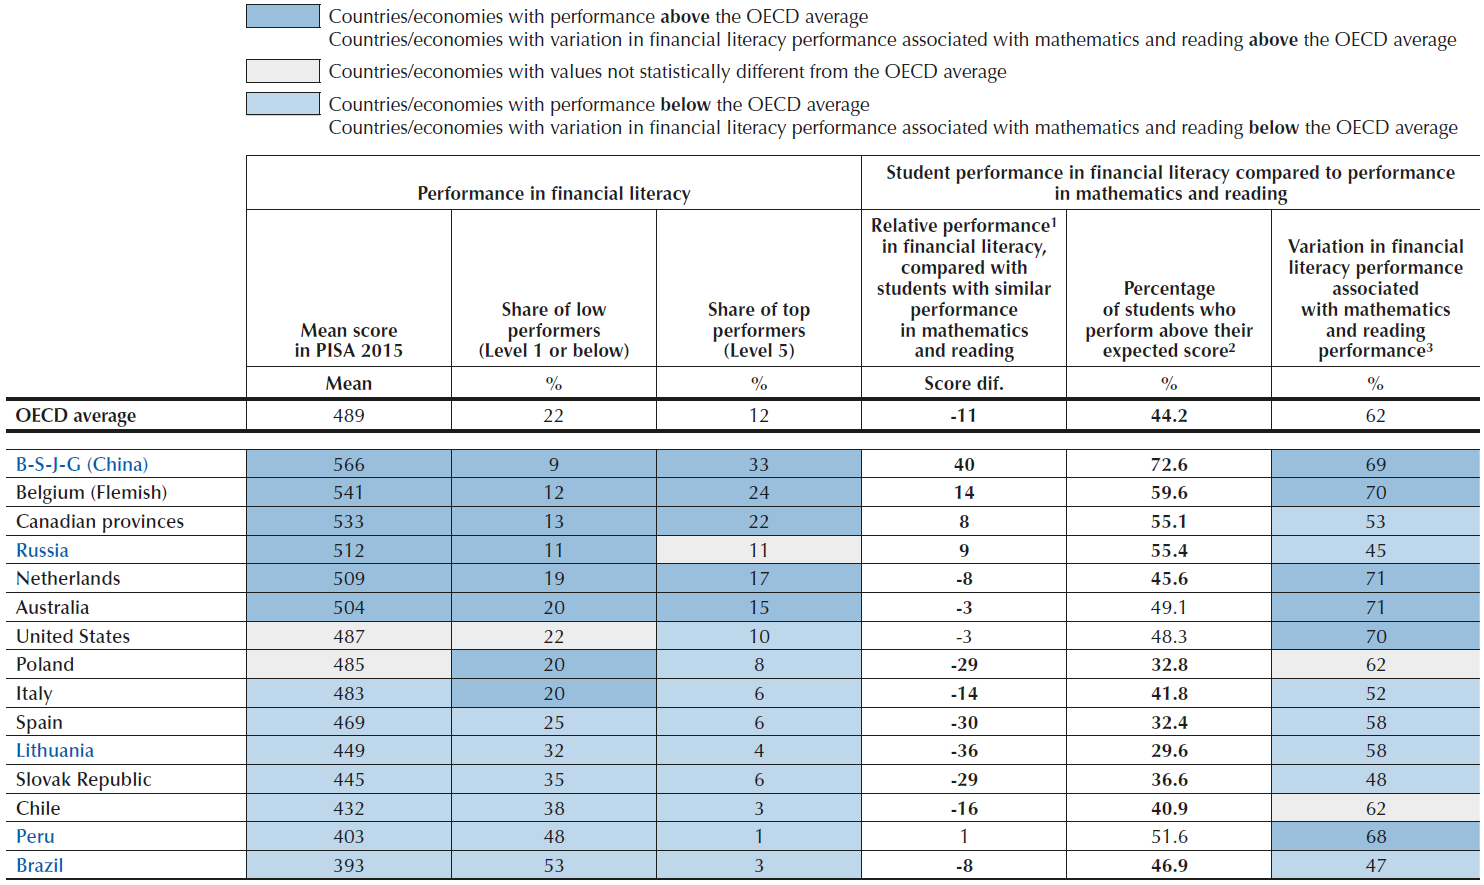
\includegraphics[width=1.0\textwidth]{tabela01-pisa2015}
\legend{\footnotesize Fonte: \citeauthor{oecd2015}, 2015, Figure IV.1.1,p.31}
\label{tab: OECD, PISA 2015, Figure IV.1.1, p.31}
\end{minipage}
\end{table}

\newpage
As duas pesquisas demonstram que falar sobre uso devido do dinheiro não faz parte do costume de boa parte das famílias brasileiras, principalmente, daquelas que não abordam o assunto pela falta de recursos. Portanto, é importante fomentar a educação financeira na formação do cidadão brasileiro, para que este possa obter conhecimento sobre o complexo sistema financeiro que interfere diretamente em sua vida. Entretanto, nos currículos dos cursos no ensino médio integrado da RFEPCT não consta a educação financeira como disciplina, exceto nos projetos pedagógicos das instituições que possuem cursos na área de finanças como os técnicos em administração ou logística integrados ao ensino médio, que parcialmente adotam o ensino de finanças.

Deste modo, projetos de pesquisa que visam incentivar, desenvolver e explorar metodologias no processo de ensino e aprendizagem voltados à educação financeira são extremamente importantes para facilitar a obtenção do conhecimento, para que o estudante possa relacionar-se melhor com o dinheiro e usufruir serviços financeiros de forma consciente, contribuindo deste modo também para a economia nacional.

\newpage

\section{Estrutura do Trabalho}
Este trabalho está organizado em seis capítulos, com o intuito de apresentar a bases teóricas e tecnológicas necessárias para a elaboração desta dissertação.

O Capítulo 1 é composto pela a introdução, a hipótese, o problema de pesquisa, os objetivos do estudo (primários e secundários), a justificativa e a descrição da estrutura do texto deste trabalho.

No Capítulo 2 são apresentados os trabalhos relacionados com a educação financeira, tecnologias educacionais e o ensino médio integrado nos institutos federais.

Já o Capítulo 3 aborda o referencial teórico relativo aos temas fundamentais do estudo: educação financeira, as políticas da educação financeira nacional adotadas pelo governo brasileiro, a composição da RFEPCT e os Institutos Federais, a construção do saber da educação financeira através da epistemologia genética e construtivismo de Piaget, por derradeiro as tecnologias educacionais utilizadas na concepção da metodologia por intermédio dos jogos sérios.

O Capítulo 4 contempla os aspectos metodológicos de tipologia da pesquisa quanto à sua natureza, aos objetivos, a análise dos dados, à finalidade e procedimentos.

Em seguida, no Capítulo 5 são expostos os detalhes do curso de Introdução à Educação Financeira para Jovens do ensino médio integrado, com as unidades temáticas, atividades e os conteúdos específicos. Por fim, o Capítulo 6 relata os resultados parciais da pesquisa.

\chapter{Análise dos Trabalhos Relacionados}
No intuito de averiguar a utilização de jogos como apoio à educação financeira em metodologias apuradas no ensino médio integrado no Brasil, bem como, para encontrar possíveis demandas, propor e justificar a elaboração do presente trabalho e de seu produto, buscou-se encontrar estudos acadêmicos nas bases de teses e dissertações da Universidade Federal do Rio Grande do Sul (Lume), da Biblioteca Digital de Teses e Dissertações (BDTD) e do Catálogo de Teses e Dissertações (CAPES), para isso utilizou-se o termo de busca “\textit{(Alfabetização OR Letramento OR Educação OR Matemática) AND Finan* AND "Ensino Médio" AND (Jogo OR Jogos OR Game OR Games)}”. Devido a ambiguidade na definição da alfabetização e educação financeira nos trabalhos acadêmicos (\citeauthor{huston2010}, \citeyear{huston2010}; \citeauthor{campos2013}, \citeyear{campos2013}), acrescentou-se ao texto da busca os termos “\textit{alfabetização}”, “\textit{letramento}” e “\textit{matemática}”, por encontrar apenas dois estudo relacionados ao “\textit{ensino médio integrado}” esta parte do termo de busca foi alterado para “\textit{ensino médio}”, tais decisões foram tomadas para aumentar o número de trabalho relacionados e qualificar o presente estudo. A busca nas bases retornou um total de 28 resultados relacionados ao termo, alguns estudos estavam presentes em mais de uma base.

O presente estudo possui como pilares a educação financeira, o ensino médio regular e os jogos sérios, por isso após a leitura do título e do resumo dos trabalhos, foram excluídos alguns estudos:

\begin{enumerate}
    \item Os projetos não relacionados, diretamente, aos 3 pilares deste estudo;
    \item Os estudos voltados apenas à matemática financeira;
    \item As dissertações e teses associados à educação de adultos.
\end{enumerate}

Após as exclusões foram encontradas cinco dissertações de mestrado, as quais foram consultadas, consideradas na construção deste estudo e estão descritas no quadro \ref{quad: quadro-01-trabalho-relacionado}. As dissertações possuem pilares semelhantes ao presente estudo, por isso foram consideradas como trabalhos relacionados.

\graphicspath{{quadros/}}
\begin{quadro}[!ht]
\centering
\begin{minipage}{1\textwidth}
\caption{Trabalhos Relacionados}
\centering
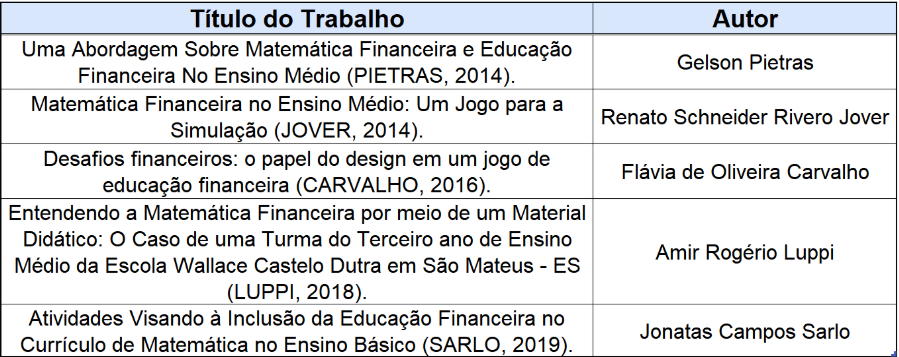
\includegraphics[width=1\textwidth]{quadro-01-trabalho-relacionado.png}
\legend{\footnotesize Fonte: O autor, 2019}
\label{quad: quadro-01-trabalho-relacionado}
\end{minipage}
\end{quadro}

\newpage
A dissertação de Gelson Pietras (\citeyear{pietras2014}), propõe uma abordagem para apresentação de alguns assuntos referente à educação financeira para o ensino médio, entre os quais podemos destacar: matemática financeira, desejos, hábitos de consumo, poupança, dívidas, compras, capitalização e investimentos, por intermédio de uma sequência de atividades práticas com cálculos de juros entre outros, em uma destas atividades utiliza o jogo “Banco Imobiliário” no processo de aprendizagem para que os alunos possam colocar em prática os conhecimentos adquiridos de forma lúdica. O autor concluiu que as atividades trouxeram ponderação sobre os hábitos financeiros mais comuns o que auxiliará nas próximas decisões de compra dos alunos.

Com o título “Matemática Financeira no Ensino Médio: um Jogo para Simulação”, Renato Schneider Rivero Jover (\citeyear{jover2014}) tem o intuito de promover a educação financeira de estudantes do ensino médio com uma metodologia baseada no jogo “Investindo na Vida”, com a fundamentação teórica financeira apresentada por Robert Kiyosaki e concepções pedagógicas de Maria Montessori, Ovide, Décroly, Lev Vygotsky, Jean Piaget e Donald Winnicott, também apresenta alguns artigos em sua dissertação para enfatizar a importância do lúdico na educação. A metodologia aborda o consumo, operações do mercado, ações e investimentos, assim como, aponta a importância da educação financeira para a formação social do indivíduo e a utilização jogos para auxiliar na aprendizagem.

A pesquisa apresentada por Flávia de Oliveira Carvalho (\citeyear{flavia2016}) em sua dissertação de mestrado, “Desafios Financeiros: o Papel do Design de um Jogo de Educação Financeira”, tem objetivo de analisar o processo de construção do jogo “Desafio Financeiros” como material pedagógico no ensino médio, visando contribuir na formação cidadã-crítica do jovens em relação aos hábitos de consumo destes. No resultado do trabalho demonstra que o jogo contribuiu no processo de aprendizagem dos alunos.

\newpage

O estudo desenvolvido por Almir Rogério Luppi (\citeyear{luppi2018}), “Entendendo a Matemática Financeira por meio de um material didático: o caso de uma turma do terceiro ano de Ensino Médio da Escola Wallace Castelo Dutra em São Mateus - ES”, apresenta conceitos básicos do sistema financeiro e os conteúdos oficiais da educação brasileira que focam nos conteúdos da matemática financeira, por meio de Tecnologias da Informática e Comunicação (TICs), jogos e dinâmica em grupos. O trabalho aponta juros compostos e sistema de amortização como os tópicos mais comuns, normalmente ensinados com o auxílio da calculadora HP12C, planilhas eletrônicas ou em softwares matemáticos como o Geogebra. Na pesquisa o autor utiliza-se do Jogo “Super Banco Imobiliário” para colocar em prática de forma lúdica alguns conceitos. Luppi (\citeyear{luppi2018}) afirma que a metodologia proporcionou noções importantes da matemática financeira aos alunos participantes e contribuiu para a Estratégia Nacional de Educação Financeira.

Jonatas Campos Sarlo (\citeyear{sarlo2019}) apresenta um estudo sobre a educação financeira e propõe atividades pedagógicas com recursos diferenciados como teatro, simulações de situações-problemas e jogos eletrônicos, como o “Jogo da Bolsa” com objetivo de auxiliar no desenvolvimento da autonomia do aluno em suas escolhas financeiras, bem como enriquecer as prática pedagógica em metodologias de ensino e aprendizagem da educação financeira. Em suas considerações finais Sarlo (\citeyear{sarlo2019}) conta que o objetivo de sua pesquisa foi alcançado com a metodologia desenvolvida, também aponta o interesse dos alunos para a temáticas das aulas principalmente quando estas envolviam tecnologias digitais.

Com base nos levantamentos e estudos, no pressuposto do trabalho, problema de pesquisa e na tese para resolver este problema, um curso para educação financeira deve contemplar as unidades temáticas relacionadas à matemática financeira, ao consumo consciente, aos serviços financeiros, às aplicações financeiras e a psicologia financeira. O quadro \ref{quad: quadro-02-trabalho-relacionado_x_unidade-tematica} apresenta os trabalhos relacionado com suas respectivas unidades temáticas.

\graphicspath{{quadros/}}
\begin{quadro}[!ht]
\centering
\begin{minipage}{1\textwidth}
\caption{Trabalhos Relacionados e Unidades Temáticas}
\centering
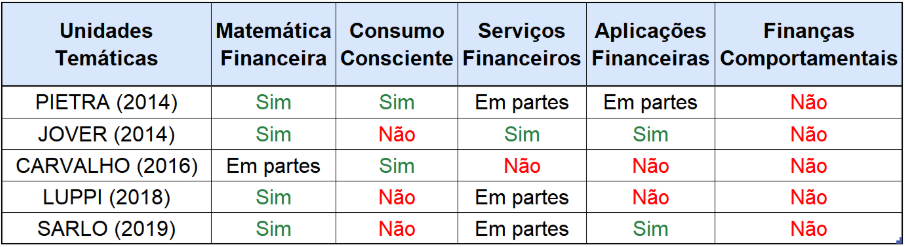
\includegraphics[width=1\textwidth]{quadro-02-trabalhos-relacionados_x_unidades-tema.PNG}
\legend{\footnotesize Fonte: O autor, 2020}
\label{quad: quadro-02-trabalho-relacionado_x_unidade-tematica}
\end{minipage}
\end{quadro}

\newpage

Ao observar o quadro \ref{quad: quadro-02-trabalho-relacionado_x_unidade-tematica}, é possível perceber uma lacuna no ensino da educação financeira a qual o presente estudo propõe solucionar, o ensino e aprendizagem de finanças comportamentais ou economia comportamental. Com o intuito de alcançar este propósito, são utilizados jogos sérios que reproduzem ambientes e relações financeiras, disponibilizando por meio destes problemas, decisões e desafios relacionados a finanças pessoais. Através da interação dos alunos com os jogos pretende-se facilitar a aprendizagem de conceitos introdutórios complexos de finanças comportamentais, como os aspectos psicológicos do comportamento humano, para auxiliar aos discentes na obtenção de bons hábitos e comportamentos financeiros para que possam alcançar a alfabetização financeira.

\chapter{Referencial Teórico}
No presente capítulo serão abordados os aspectos teóricos, epistemológicos e tecnológicos inerentes ao tema da pesquisa, à elaboração do curso de Introdução à Educação Financeira para Jovens do ensino médio integrado da RFEPCT e sua metodologia.

A educação financeira, as políticas públicas nacionais voltadas à educação financeira, os aspectos relevantes à epistemologia e os jogos educativos, chamados também de jogo sérios, são os temas principais do referencial teórico nos trabalhos relacionados (PIETRA, \citeyear{pietras2014}; JOVER, \citeyear{jover2014};  CARVALHO, \citeyear{flavia2016}; LUPPI, \citeyear{luppi2018}; SARLO, \citeyear{sarlo2019}), por isso também são explorados neste capítulo, bem como a RFEPCT, o Instituto Federal Sul-rio-grandense e seu campus na cidade de Gravataí, local onde foi aplicado à pesquisa do estudo de caso.

\section{Educação Financeira}
O Banco Central do Brasil (BACEN) é integrante do Comitê Nacional de Educação Financeira (CONEF) e uma das principais instituições do Sistema Financeiro Nacional (SFN).

Segundo o BACEN (\citeyear{bacen2013}) os temas principais abordados na educação financeira são o Consumo Consciente (Desejos x Necessidades), Planejamento Orçamentário, Crédito e Dívidas, Poupança e Investimentos, Seguros e Previdência, tais assuntos serão descritos no decorrer deste capítulo e objetos de estudo no processo de ensino e aprendizagem do presente projeto.

\subsection{Consumo Consciente e Finanças Comportamentais}
Segundo Buaes, Comerlato e Doll (\citeyear{buaes2015}) “entre o sonho de ter e a possibilidade de comprar é possível planejar o consumo. Esse é chamado de consumo consciente ou consumo planejado”. Em outras palavras, o consumo consciente, em finanças, compreende a utilização dos recursos de forma planejada, com planos de curto, médio e longo prazos bem definidos para evitar gastos desnecessários ou desperdício de recursos.

Entretanto, aplicar os conceitos do consumo consciente pode ser difícil, pois, as emoções e habilidades interferem diretamente nas decisões financeiras afetando o nosso ganho, gasto e dinheiro poupado \cite{martins2004}. Diante disso, é extremamente importante entender os fatores comportamentais humano relacionado ao consumo financeiro.

O conhecimento estudado pela economia comportamental é relativamente novo e engloba aspectos da economia e psicologia. Também chamada de finanças comportamentais, a economia comportamental tem o objetivo de explicar a análise econômica e/ou financeira das pessoas por intermédio pressupostos psicológicos \cite{castro2014}, em outras palavras as finanças comportamentais têm o interesse de explicar as tomadas de decisões financeiros das pessoas através de aspectos psicológicos do comportamento intrapessoal.

O Nobelista Econômico Daniel Kahneman (\citeyear{kahneman2012}) afirma que até a década de 1970 os cientistas entendiam que em geral as pessoas eram racionais e as emoções eram responsáveis por afastarem as pessoas da realidade. Entretanto, o artigo escrito por Kahneman e Tversky “Julgamento sob incerteza: heurísticas e vieses” (\citeyear{kahneman1974}, tradução nossa), descreve atalhos mentais que simplificam o pensamento de modo intuitivo e comprovam erros cognitivos do comportamento humano não um afastamento simples da realidade causado pelas emoções. Os autores também explicam vieses, erros sistemáticos e previsíveis em algumas circunstâncias, como manifestações de heurísticas, atalhos mentais que agilizam e simplificam o processo de percepção e avaliação de informações para tomada de decisões.

Ademais, heurísticas e vieses afetam inclusive a tomada de decisões financeiras das pessoas \cite{kahneman2012}, por esse motivo, estratégias e técnicas de vendas utilizam-se destes atalhos mentais para estimular o consumidor a realizar gastos não planejados, tais estímulos são chamados de gatilhos mentais no marketing \cite{cialdini2012}.

Nessa perspectiva, o psicólogo Kahneman (\citeyear{kahneman2012}) sugere que o ser humano possui duas formas distintas para planejar e executar as ações: o Pensamento Rápido e o Pensamento Lento. O primeiro é emocional, intuitivo, impulsivo, involuntário e valoriza o presente, enquanto o segundo é racional, dedutivo, lento, consciente e valoriza o futuro.

Estratégias e técnicas de vendas utilizam gatilhos mentais para estimular a compra, visando se aproveitar do pensamento rápido. Segundo Cialdini (\citeyear{cialdini2012}), há diversos gatilhos mentais, por exemplo o gatilho da escassez que ocorre quando um produto ou serviço é divulgado com poucas unidades, ou o gatilho da urgência quando a oportunidade de compra é limitada por um pequeno interstício, ambos gatilhos mentais exploram um viés comportamental do ser humano a aversão à perda (ARIELY, \citeyear{ariely2010}; KAHNEMAN, \citeyear{kahneman2012}), desta forma os clientes são estimulados a adquirir produtos ou serviços por medo de perder uma “oportunidade”, por fim efetuam a compra baseado no pensamento rápido que foi incentivado por um gatilho mental, sem perceber a influência das técnicas de compras, por isso a importância de planejar o consumo para enfim obter um consumo consciente. Para atingir este objetivo é extremamente importante a realização de um planejamento orçamentário.

\subsection{Planejamento Orçamentário}
O planejamento orçamentário ou orçamento é uma ferramenta para o planejamento financeiro pessoal ou familiar onde deve constar todas as receitas fixas e variáveis (entrada monetária), despesas fixas e variáveis (saída monetária) utilizado para decidir quais serão as prioridades de consumo pessoal ou de uma família.

\newpage
\begin{citacao}
O orçamento permite o planejamento de como gastar o seu dinheiro e mesmo economizar e investir. Após listar detalhadamente todas as receitas e despesas, é preciso fazer o balanço do mês, para saber quanto sobra, quanto falta ou se há equilíbrio entre ganhos e gastos. O orçamento possibilita o planejamento financeiro, ou seja, escolher em que e como vai gastar a partir da definição de suas prioridades, além de ajudar a administrar os imprevistos e reduzir o consumo desnecessário e indesejado. (BUAES, COMERLATO e DOLL, \citeyear{buaes2015}).
\end{citacao} 

Por isso é tão importante o planejamento orçamentário na realização do consumo consciente, dos objetivos, do controle financeiro pessoal e familiar, sem o orçamento financeiro a possibilidade de ocorrer endividamento excessivo aumenta, dificultando o pagamento das dívidas, o que pode provocar a inclusão do nome em lista de proteção de crédito.

Segundo o Banco Central do Brasil (\citeyear{bacen2013}), o orçamento pode ser dividido em 4 (quatro) etapas: planejar, registrar, agrupar e avaliar. Planejar consiste no levantar todas as receitas e despesas, estabelecendo um limite para cada categoria de gasto, o ideal é diminuir o valor das despesas ao máximo possível e que este não ultrapasse o valor das receitas, pois assim sobrará mais verba para poupar. Registrar todas as despesas e receitas diárias é fundamental para o planejamento orçamentário, inclusive as despesas de valores menores, visto que, somados ao fim do mês podem gerar gastos elevados, por muitas vezes estes valores não são considerados, contudo também afetam o orçamento. Esse registro pode ser feito através de planilhas eletrônicas, aplicativos \textit{mobile} ou qualquer \textit{software} para facilitar as anotações. Agrupar as despesas e receitas anotadas em grupo, ou seja, separar cada movimentação em categorias como alimentação, moradia, saúde, mercado, compras, educação, rendimento, remuneração etc., a organização de categorias pode também ser classificada no momento do registro. Por último avaliar se as metas máximas de consumo e receitas planejadas foram alcançadas em todas categorias, o ideal é que a soma dos gastos não ultrapasse o valor total das receitas, a repetição contínua deste ciclo provê a continuação de um consumo consciente evitando a solicitação de créditos o que pode causar dívidas.

\subsection{Crédito e Dívidas}
A utilização do crédito é muito comum entre a população brasileira para realizar compras de produtos, serviços, bens de consumo, imóveis, veículos etc. Contudo, o que é o crédito? Segundo o BACEN (\citeyear{bacen2013}, p. 25): “O crédito é uma fonte adicional de recursos que não são seus, mas obtidos de terceiros (bancos, financeiras, cooperativas de crédito e outros), que possibilita a antecipação do consumo para aquisição de bens ou contratação de serviços”. Em outros termos, crédito é o empréstimo de valor monetário de terceiros a consumidores quando estes não possuem ou não querem utilizar recursos próprios para aquisição de bens, serviços, produtos e outros. Existem diversas modalidades de crédito como cheque especial, empréstimos pessoais, financiamentos, cartão de crédito, crédito consignado, compra a prazo em lojas, entretanto toda a modalidade de adiantamento financeiro cobra um valor adicional além do emprestado, chamado de juros, quantia cobrada pelo aluguel do dinheiro ao consumidor que encarece o preço final.

A dívida é todo o compromisso financeiro realizado através de crédito em compras parceladas de produtos, serviços, bens de consumo, imóveis etc., o excesso de dívidas, a falta de consumo consciente e de um plano orçamentário pode acarretar no atraso de pagamentos, ou pior, o não pagamento das dívidas e neste momento o consumidor tornar-se-á inadimplente passível de ter o seu nome inscrito em órgãos de proteção ao crédito como o SCPC (Serviço Central de Proteção ao Crédito) que dificultará a obtenção de novos créditos. Para Gustavo Cerbasi (\citeyear{cerbasi2015}), a melhor forma de comprar um produto ou serviço é poupar e investir mensalmente até obter o valor total do item, evitando contratar créditos que comprometem o poder de compra dos meses posteriores.

Segundo Bortoluzzi et al (\citeyear{bortoluzzi2015}), a partir de 2003 o Brasil sofreu transformações no modelo econômico e social, que possibilitou grandes mudança para a sociedade brasileira. Nesse modelo as medidas políticas propuseram redução na taxa de juros, ampliação do volume de crédito direcionado às empresas e famílias, tornando o crédito mais acessível à população. Entretanto, os autores apontam que esta facilidade de acesso ao crédito e a falta da educação financeira provocaram um aumento no índice do endividamento. Sendo assim, a facilidade na contratação de crédito, a falta da educação financeira e o grande apelo ao consumo do marketing, pode transformar-se em armadilha para o consumidor, pois de acordo com Zaremba (\citeyear{zaremba2007}), a maior parte das pessoas age como se não conhecessem que pagar juros abusivos podem acarretar em problemas financeiros.

\subsection{Poupança e Investimentos}
O orçamento pessoal ou familiar pode ser avaliado de forma geral calculando a diferença entre o total de entrada monetária (receita) e o total de saída monetária (despesa). Desta forma quando:
\begin{itemize}
    \item A despesa é maior que a receita o orçamento é deficitário;
    \item A despesa for igual a receita o orçamento é neutro;
    \item A receita é maior que a despesa o orçamento é superavitário.
\end{itemize}

Segundo o Banco do Brasil (\citeyear{bb2012}, p. 24): “Quando a pessoa não consome toda a sua renda, essa sobra poderá ser transformada em poupança”, portanto todo orçamento superavitário produz uma sobra financeira chamada de poupança, normalmente confundido com Caderneta de Poupança que é a aplicação mais popular no Brasil.

O investimento ou aplicação ocorre quando o dinheiro poupado é utilizado para gerar mais dinheiro, por isso é considerado um ativo. Existem diversos tipos de aplicações financeiras no Brasil, os mais comuns são a Caderneta de Poupança, Certificados de Depósito Bancário (CDB), Recibo de Depósito Bancário (RDB), Letras de Crédito (LC), Letras de Crédito Imobiliário (LCI) e Letras de Crédito do Agronegócio (LCA), Debêntures, Títulos Públicos, Ações, Fundos e Clubes de Investimentos.

Todo o investimento possui três componentes: liquidez, risco e rentabilidade, de acordo com BACEN (\citeyear{bacen2013}), a liquidez é a capacidade de um investimento ser transformado em dinheiro, em qualquer tempo por um preço justo. O risco é a possibilidade de ocorrer perda no valor investido e a rentabilidade é a remuneração que o investimento retorna ao investidor. Quanto maior o risco, maior é a possibilidade de ocorrer perdas de capital, entretanto maior poderá ser a rentabilidade também.

Quanto a rentabilidade, os investimentos se caracterizam como renda fixa e/ou renda variável. Na renda fixa a remuneração paga é correspondente a uma taxa de juros determinada na contratação, já na renda variável não é possível determinar uma taxa de remuneração na contração \cite{bacen2013}. Em outras palavras, o investidor que contrata uma aplicação de renda fixa sabe qual será a taxa de juros acordada, ao contrário da renda variável onde a rentabilidade será determinada no momento da venda do ativo, o que pode inclusive incorrer em perdas do montante aplicado. Ao realizar um plano de investimento é importante considerar o risco, a liquidez, a rentabilidade, o tipo da aplicação e a finalidade dos recursos investido de acordo com o objetivo de cada investidor.

\subsection{Seguros e Previdência}
A Superintendência de Seguros Privados (Susep), órgão federal brasileiro responsável por fiscalizar e controlar empresas de seguros e previdência privada, afirma que seguro é o:

\begin{citacao}
Contrato mediante o qual uma pessoa denominada Segurador, se obriga, mediante o recebimento de um prêmio, a indenizar outra pessoa, denominada Segurado, do prejuízo resultante de riscos futuros, previstos no contrato \cite{susep2007}.
\end{citacao}

A vida é imprevisível em boa parte, eventos (positivos ou negativo) não planejados, inesperados ou impensáveis podem ocorrer com qualquer ser humano. Entre os eventos ruins pode-se citar exemplos como: doenças, acidentes, morte, desemprego, furtos ou roubos de bens entre outros. Por isso, a importância da contratação de um seguro, com objetivo de diminuir o prejuízo financeiro causado por eventuais problemas inesperados. Para isso, as seguradoras oferecem diversos tipos de seguros com respectivos planos, benefícios e contratos, entre os principais destaca-se o de vida, residencial, veicular, empresarial e viagem.

Da mesma forma a previdência em finanças é a preparação econômica durante um determinado período para lidar com situações do futuro como aposentadoria ou realização de projetos (BANCO DO BRASIL, \citeyear{bb2015}). Atualmente existem dois tipos de regimes para prover recursos financeiros: a Previdência Social, administrada pelo Instituto Nacional de Seguro Social, e a Previdência Privada, oferecida por bancos e seguradoras e supervisionada pela Susep.

\section{Políticas da Educação Financeira Nacional}
O intuito deste capítulo é apresentar o levantamento sobre as políticas públicas educacionais nacionais voltadas para o desenvolvimento da educação financeira, especificamente os projetos de leis sobre a educação financeira que tramitam no Congresso Nacional, a Estratégia Nacional de Educação Financeira - ENEF, as propostas da Base Nacional Comum Curricular - BNCC para o ensino de finanças na educação básica.

\subsection{Projetos de Lei Sobre a Educação Financeira}
Na Câmara dos Deputados, casa iniciadora de leis no Brasil, existem 12 de projetos de lei, entre 2004 a 2019, cujo conteúdo propõe a inclusão ou criação da educação financeira como componente curricular na educação básica (ensino fundamental e médio). Neste levantamento considerou-se apenas os projetos da Câmara dos Deputados, por ser a casa iniciadora de leis federais.

O primeiro Projeto de Lei o PL 3401/2004 foi arquivado tal como o PL 306/2007, outros nove projetos (PL 3421/2012, PL 7155/2014, PL 3590/2015, PL 3691/2015, PL 4215/2015, PL 4915/2016, PL 7318/2017, PL 239/2019, PL 3114/2019), por tratarem de temáticas idênticas, foram apensados (unidos), diretamente ou indiretamente, ao PL 2107/2011 que se encontra na Comissão de Educação (CE), sendo este projeto o único em pauta, tornando-o principal relacionado à educação financeira no Congresso Nacional.

O Projeto de Lei PL 2107/2011 possui como proposta “alterar a lei de diretrizes e bases da educação nacional, incluindo a disciplina de Noções de Educação Financeira como conteúdo obrigatório no ensino médio” \cite{brasil2011}. Além disso, estabelece o interstício de 3 anos para os sistemas de ensino se adequarem às exigências descritas \cite{brasil2011}, todavia, não aborda a educação financeira para o ensino fundamental.

Ao analisar o histórico dos projetos de lei voltados à educação financeira, observa-se que o primeiro trabalho foi proposto em 2004, há 16 anos, e até a elaboração deste estudo nenhum projeto foi transformado em lei.

É importante para o bem-estar social, a economia e os estudantes da educação básica que os congressistas brasileiros tratem deste assunto, essencial para a formação cidadã, com uma maior celeridade.


\subsection{A Estratégia Nacional de Educação Financeira}
Entre as diversas iniciativas para promover o letramento financeiro destaca-se a Estratégia Nacional de Educação Financeira (ENEF), instituída pelo governo brasileiro através do Decreto nº7.397, de 22 de dezembro de 2010, sob a responsabilidade do Comitê Nacional de Educação Financeira (CONEF) com execução e coordenação dos programas realizadas pela Associação de Educação Financeira do Brasil (AEF-Brasil). Tal estratégia tem a finalidade de fortalecer a cidadania, aumentar a eficiência e solidez do Sistema Financeiro Nacional (SFN), disseminar a educação financeira e previdenciária, promover as decisões financeiras de forma consciente e autônomas, bem como atuar com informação, orientação e formação de forma gratuita visando o interesse público, por intermédio de dois documentos norteadores: Orientações para Educação Financeira nas Escolas e Orientações para Educação Financeira de Adultos \cite{enef2010}. Através da ENEF são executados projetos de cursos, blogs, vídeos, livros, jogos, material de apoio aos professores do ensino médio e fundamental, a Semana da Educação Financeira e o Mapeamento de Iniciativas de Educação Financeira voltadas para o desenvolvimento da educação financeira.

O CONEF, também constituído pelo Decreto nº7.397, é composto pelo Diretor do Banco do Brasil, Presidente da Comissão de Valores Mobiliários, Diretor-Superintendente da Superintendência Nacional de Previdência Complementar, Superintendente da Superintendência de Seguros Privados, Secretário-Executivo do Ministério da Fazenda, Secretário-Executivo do Ministério da Educação, Secretário-Executivo do Ministério do Trabalho e Previdência Social e o Secretário Nacional do Consumidor do Ministério da Justiça. Observa-se nesta composição a presença dos principais órgãos federais relacionados às finanças, economia e trabalho. Compete ao CONEF promover a educação financeira através de planos, metas, programas, ações, financiamento, execução de projetos e revisão da ENEF \cite{brasil2010}.

A AEF-Brasil é uma Organização da Sociedade Civil de Interesse Público (OSCIP), com certificação do Ministério da Justiça, composta por quatro instituições do mercado financeiro: Associação Brasileira das Entidades dos Mercados Financeiros e de Capitais (ANBIMA); Brasil, Bolsa, Balcão (B3); Confederação Nacional das Empresas de Seguros Gerais, Previdência Privada e Vida, Saúde Suplementar e Capitalização (CNSeg); e Federação Brasileira de Bancos (FEBRABAN). Por convênio de cooperação técnica com o CONEF, a AEF-Brasil é responsável por executar e coordenar todos os programas propostos pela ENEF e tem o objetivo de promover a educação financeira nacional e de tecnologias socioeducacionais nesta área \cite{aefbrasil2011}. A AEF-Brasil é uma associação sem fim lucrativo e recebe apoio financeiro de instituições privadas, do governo e da sociedade civil que compreendem a importância da educação financeira.

\subsection{A BNCC e a Educação Financeira}
A Constituição do Brasil de 1988 prevê a elaboração de conteúdos mínimos para o ensino fundamental a fim de assegurar formação básica comum nacional, entretanto somente em 1996 é aprovada a Lei 9.394/1996 que regula a base nacional comum para o ensino básico em todos sistemas de ensino \cite{brasil1996}. Entre os anos 1997 à 2012 são lançados os Parâmetros Curriculares Nacionais (PCN), as Diretrizes Curriculares Nacionais Gerais para o ensino básico (DCNs) e os Parâmetros Curriculares Nacionais para o Ensino Médio (PCNEM) “com o objetivo de cumprir o duplo papel de difundir os princípios da reforma curricular e orientar o professor, na busca de novas abordagens e metodologias.” \cite{brasil2017b}. Em 2014 o Ministério da Educação e Cultura iniciou a elaboração da BNCC visando estabelecer os ensinamentos básicos para o desenvolvimento de conhecimentos necessários para o exercício da cidadania. No ano de 2015 foi disponibilizada a primeira versão da BNCC, consequentemente, iniciou-se uma mobilização entre as instituições de ensino para a discussão sobre a BNCC. Após dois anos de debates e mudanças, a BNCC foi homologada pelo Ministério da Educação (MEC) em 20 de dezembro de 2017 e apresentava orientações sobre conceitos básicos da educação financeira como economia, finanças, taxas de juros, inflação, aplicações financeiras e impostos, com o intuito de unificar o processo de ensino e aprendizagem, além de tornar o ensino da educação financeira obrigatório em todas as instituições de ensino até 2020.

Segundo a BNCC nas séries iniciais do ensino fundamental, do 1ª ao 4ª ano, deve-se trabalhar com os estudantes especificamente a unidade temática “Grandezas e Medidas” concentrando-se no reconhecimento, conversões e resolução de problemas do sistema monetário brasileiro, habilidades estas que estão ligadas à matemática financeira. A partir do 6º ano, o tema retorna ao currículo e permanece até o fim do ensino fundamental através das unidades temáticas “Números” e “Grandezas e Medidas”, trabalhando as habilidades EF06MA13, EF06MA32, EF07MA02, EF07MA02 e a EF09MA05 que descreve:

\begin{citacao}
Resolver e elaborar problemas que envolvam porcentagens, com a ideia de aplicação de percentuais sucessivos e a determinação das taxas percentuais, preferencialmente com o uso de tecnologias digitais, no contexto da educação financeira. \cite{brasil2017c}.
\end{citacao}

A habilidade EF09MA05 é indicada na BNCC ao 9º ano do ensino fundamental e aborda parte da educação financeira através de uma metodologia ativa de resolução de problemas com apoio da tecnologia, o que poderá trazer estímulos maiores para aprendizagem, principalmente se o contexto do problema proposto fizer parte do cotidiano do aluno.

No mesmo sentido, no ensino médio a BNCC apresenta a matemática financeira e parte da educação financeira por meio de temas ligados a finanças pessoais e familiares como orçamento, investimentos, sustentabilidade e tomada de decisões, também com apoio de tecnologias digitais através das habilidades descritas no quadro \ref{quad: quadro-03-habilidade}.

\graphicspath{{quadros/}}
\begin{quadro}[!ht]
\centering
\begin{minipage}{1.\textwidth}
\caption{Habilidades Propostas na BNCC para Matemática  e Educação Financeira}
\centering
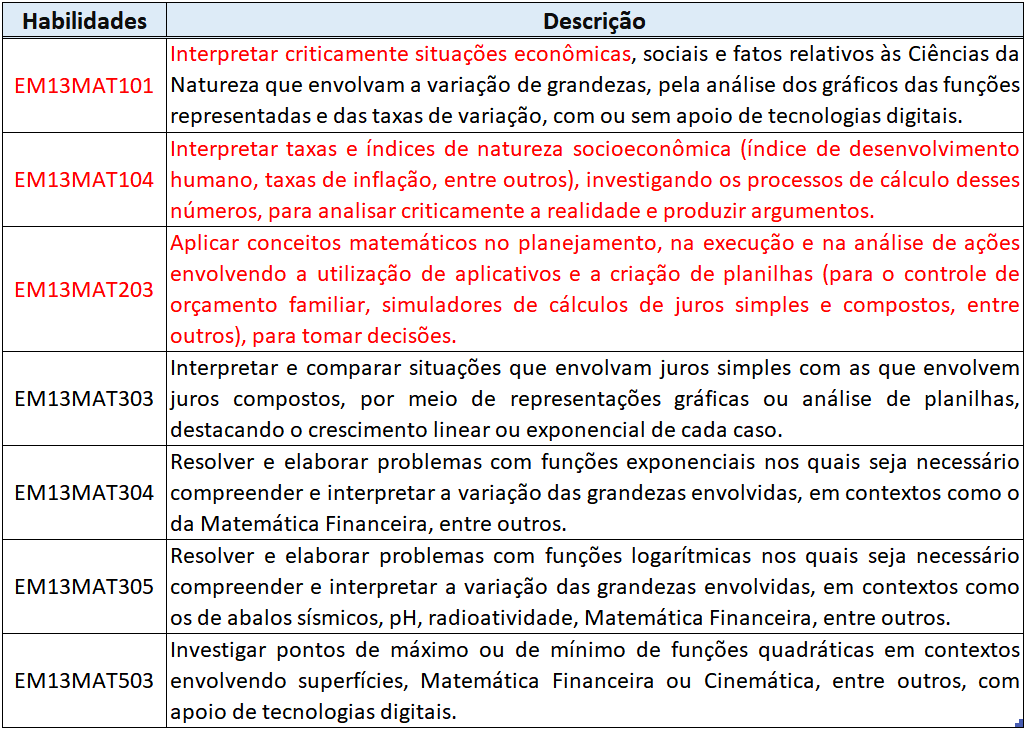
\includegraphics[width=1\textwidth]{quadro-03-habilidades.png}
\legend{\footnotesize Fonte: \cite{brasil2018} Adaptado pelo Autor}
\label{quad: quadro-03-habilidade}
\end{minipage}
\end{quadro}

\newpage
Analisando o quadro \ref{quad: quadro-03-habilidade} nota-se que as habilidades descritas e propostas na BNCC, em sua maior parte, são voltadas ao contexto da matemática financeira, exceto as habilidades EM13MAT101, EM13MAT104 e EM13MAT203 que abordam parcialmente a educação financeira, estas estão destacadas em vermelho no quadro \ref{quad: quadro-03-habilidade}.

A Base Nacional Comum Curricular apresentou pequenos avanços no incentivo a construção da educação financeira, principalmente na unidade temática relacionada à matemática financeira, por meio da inclusão de habilidades relacionadas a cálculos e funções matemáticas, todavia, Kahneman (\citeyear{kahneman2012}) afirma que pessoas podem ter a capacidade realizar cálculos financeiros com exatidão e concomitantemente ter comportamento e hábitos que lhes trazem problemas com finança. Desse modo, o indivíduo pode ser um exímio matemático financeiro e ainda assim possuir fatores comportamentais materialista, compulsivos em compras e propenso ao endividamento. Por isso, é importante aos alunos da educação básica a aprendizagem completa da educação financeira a qual engloba todas as suas unidades temáticas (matemática financeira, finanças comportamentais, consumo consciente, instituições financeiras, investimento e previdência). Desta forma, pode-se proporcionar aos alunos conhecimentos para exercer melhores escolhas financeiras para melhoria em sua qualidade de vida e bem-estar social, inclusive dos estudantes da RFEPCT local deste estudo de caso, fortalecendo assim a cidadania do país.

\section{A RFEPCT e os Instituto Federais}
A história da RFEPCT teve início em 1909 quando o Presidente Nilo Peçanha cria formalmente uma rede com 19 “Escolas de Aprendizes e Artífices”, uma em cada capital dos Estados da República, para o ensino profissional primário e gratuito, através do Decreto 7.566 em 23 de setembro \cite{brasil1909}, as quais foram inauguradas em 1910, alcançando todas as regiões do Brasil.

A educação profissional passou por diversas mudanças das quais pode-se destacar: o acesso a todos os ramos e graus (Lei 378/1937); a autonomia na organização didática e gestão em 1959; a equiparação ao ensino acadêmico (Lei 4.024/1961); o currículo do segundo grau passa a ser todo técnico-profissional (Lei 5692/71); a instituição do Sistema Nacional de Educação Tecnológica (Lei 8.948/1994); a permissão do ensino médio integrado ao técnico (Decreto 5.154/2004);  a integração a Educação de Jovens e Adultos em 2006; a instituição legal da Rede Federal de Educação Profissional, Científica e Tecnológica - RFEPCT (Lei 11.892/2008). As Escolas de Aprendizes e Artífices também sofreram alterações em sua nomenclatura, a partir de 1937 denominou-as como Liceus Profissionais (Lei 378/1937), em 1942 Escolas Industriais e Técnicas (Decreto 4.127/1942), em 1959 Escolas Técnicas, a partir de 1978 são chamadas de Centros Federais de Educação Tecnológica - CEFETS, e por derradeiro, em 2008 Institutos Federais de Educação, Ciência e Tecnologia.

Com a promulgação da Lei 11.892 em 2008, a Rede Federal de Educação Profissional, Científica e Tecnológica foi formalmente oficializada, formada por um conjunto de autarquias da administração pública indireta que possuem autonomia administrativa, patrimonial, financeira, didático-pedagógica e disciplinar, composta pelas seguintes instituições \cite{brasil2008}:

\begin{itemize}
    \item 38 Institutos Federais de Educação, Ciência e Tecnologia
    \item 3 Centros Federais de Educação Tecnológica
    \item 23 Escolas, Colégios, Centros vinculados às Universidades Federais
    \item Universidade Tecnológica Federal do Paraná
    \item Colégio Pedro II
\end{itemize}

Os institutos federais tem por objetivos: ministrar educação profissional técnica de nível médio no formato integrado, subsequente e concomitante,  privilegiando os cursos integrados, reservando no mínimo 50\% para este objetivo; realizar projetos de extensão e pesquisas aplicadas; ministrar em nível de educação superior cursos de bacharelado, tecnologia e licenciatura, bem como pós-graduação lato sensu e stricto sensu de mestrado e doutorado. Os objetivos devem estar em articulação com o mundo do trabalho, a sociedade e o desenvolvimento socioeconômico local e regional nas áreas da educação profissional e tecnológica \cite{brasil2008}. A tabela \ref{tab: tabela02-institutos} apresenta a disposição dos Institutos Federais de Educação, Ciência e Tecnologia, Colégio Pedro II, Centros Federais de Educação Tecnológica e seus campi. São ao todo 42 instituições com 632 campus que podem ministrar a educação profissional técnica de nível médio no formato integrado.

\graphicspath{{tabelas/}}
\begin{table}[!ht]
\centering
\begin{minipage}{1.\textwidth}
\caption{Disposição das Instituições de Ensino da RFEPCT}
\centering
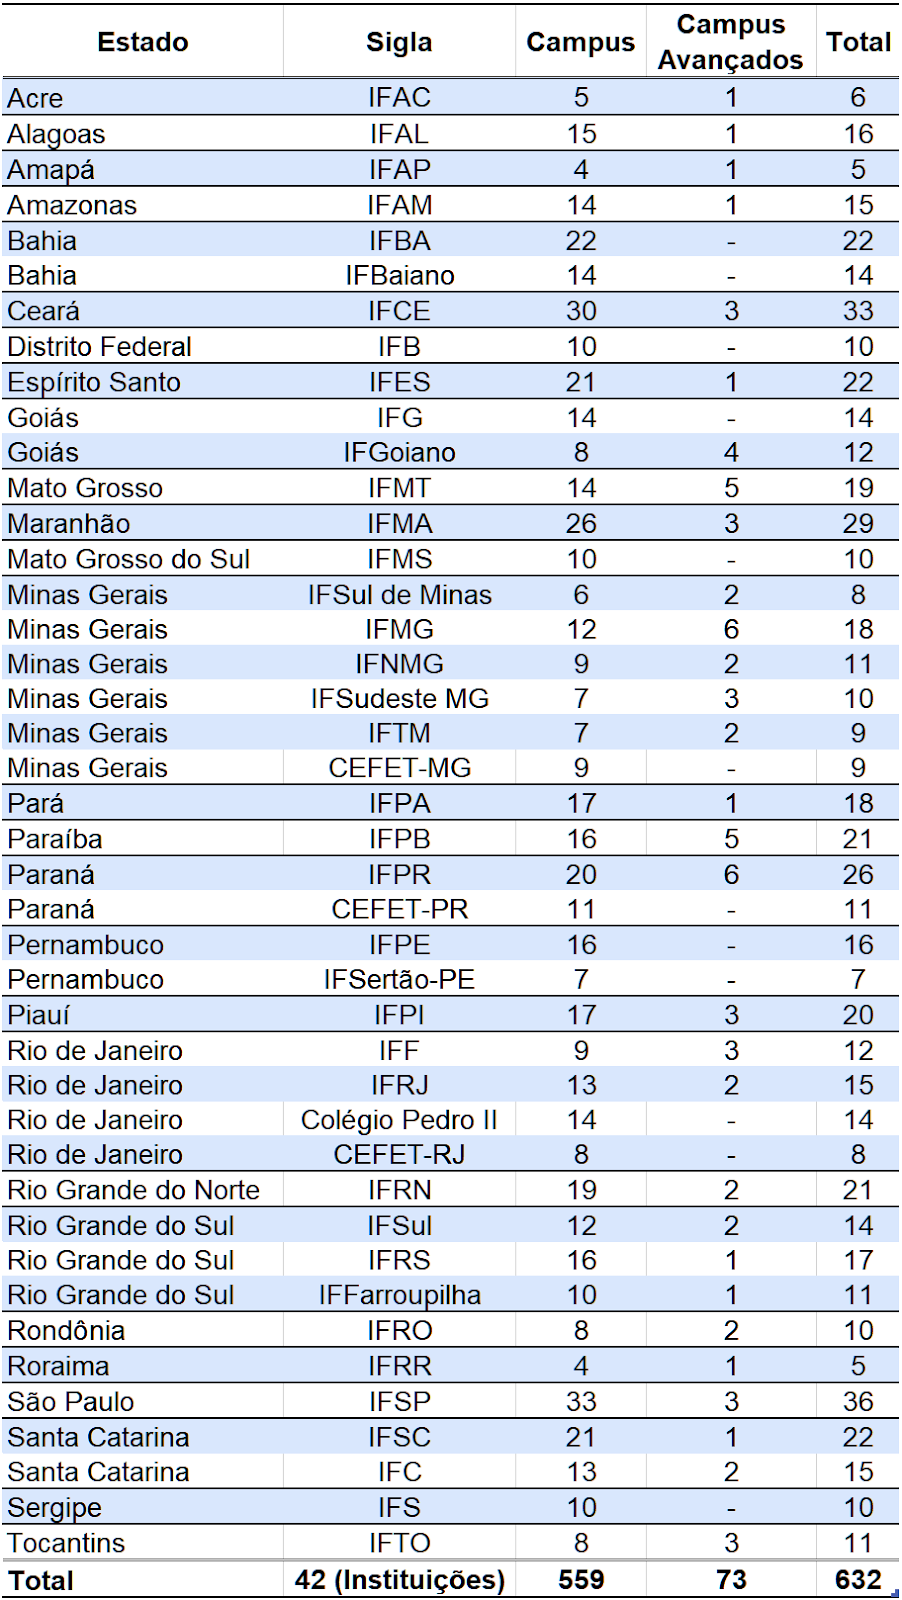
\includegraphics[width=0.7\textwidth]{tabela02-institutos.png}
\legend{\footnotesize Fonte: Dos Autores}
\label{tab: tabela02-institutos}
\end{minipage}
\end{table}

Dentro das diversas instituições de ensino da RFEPCT, listados na tabela \ref{tab: tabela02-institutos}, há o Instituto Federal Sul-rio-grandense-IFSUL local onde foi aplicada à pesquisa do presente estudo, especificamente no Campus Gravataí.

\subsection{O IFSUL e o Campus Gravataí}
No início de 1930 foi inaugurado no Rio Grande do Sul a primitiva Escola de Aprendizes e Artífices, a primeira escola federal do estado voltada ao ensino profissional, diferentemente dos outros estados do Brasil, que inauguraram suas Escolas de Aprendizes e Artífices em 1929. Assim como as outras escolas desta modalidade, a unidade do Rio Grande do Sul também sofreu e promoveu alterações políticas nos cursos oferecidos, no público atendido e na sua nomenclatura, e por intermédio da LEI Nº 11.892, em 29 dezembro de 2008, tornou-se o Instituto Federal de Educação, Ciência e Tecnologia Sul-rio-grandense - IFSUL \cite{ifsul2015}. Atualmente este instituto possui cursos técnicos (integrados, concomitante e subsequente), de graduação (licenciatura, bacharelado e tecnologia), de pós-graduação lato sensu e stricto sensu (mestrado), em diversas áreas do conhecimento, distribuídos em 14 campi (Bagé, Camaquã, Charqueadas, Gravataí, Avançado Jaguarão, Lajeado, Avançado Novo Hamburgo, Passo Fundo, Santana do Livramento, Sapiranga, Sapucaia do Sul, Venâncio Aires e Pelotas).

O Campus Gravataí iniciou as atividades no segundo semestre de 2014, com o curso Técnico Subsequente de Informática. Atualmente o campus possui cinco cursos: Pós-graduação em Educação Física Escolar, as Graduações em Análise e Desenvolvimento de Sistemas e em Formação Pedagógica para Graduados não Licenciados, o Técnico de Informática (subsequente) e o Técnico de Informática para Internet (integrado ao ensino médio) no qual foi aplicada a pesquisa do presente estudo.

Pela natureza e vocação do IFSUL, as diversas teorias educacionais e metodologias de ensino podem ser exploradas para dar suporte efetivo à formação do futuro profissional dos alunos, inclusive na construção do conhecimento da educação financeira com apoio de tecnologias educacionais e epistemologias fundamentadas.

\section{Aprendizagem e a Educação Financeira}
A educação financeira tem por objetivo o desenvolvimento de novos conhecimentos, assim como bons hábitos e comportamentos financeiros, podendo ocorrer esta educação por intermédio de um processo aprendizagem. Para Ausubel et al (\citeyear{ausubel1980}) a educação é aprendizagem orientada com objetivo de proporcionar aquisição profunda de estruturas do conhecimento e das capacidades necessárias para sua obtenção. Nessa continuidade, Cosenza e Guerra (\citeyear{cosenza2011}) argumentam que as pessoas aprendem quando apresentam novos comportamentos que permitem transformar os hábitos e o ambiente nas quais vivem. Por meio de uma teoria de aprendizagem é possível manipular e desenvolver os fatores importantes que influenciam no processo de ensino-aprendizagem (AUSUBEL et al., \citeyear{ausubel1980}). De acordo com Moreira (\citeyear{moreira2017}, p. 19) “teorias de aprendizagem são, portanto, tentativas de interpretar sistematicamente, de organizar, de fazer previsões com conhecimentos relativos à aprendizagem”, pois há uma relação entre fatores que influenciam a aprendizagem e o modo como o aluno aprende.

Em face deste conhecimento as teorias de aprendizagem buscam elaborar meios e recursos para que os alunos aprendam melhor, desenvolvendo novos conhecimentos para articular com saberes anteriores. Este trabalho se fundamenta nas teorias de aprendizagem do Epistemólogo Jean Piaget para estruturar meios e recursos com o intuito de encontrar o melhor caminho para o processo de ensino-aprendizagem da educação financeira aos alunos da RFEPCT.

Ao buscar informações sobre educação financeira, são encontradas inúmeras fontes de livros, sites, vídeos, blogs, cursos etc. sobre planejamento financeiro orçamentário, sonhos, objetivos, metas, planos, aposentadoria, despesas, receitas, dívidas, gastos, poupança, investimentos, hábitos e finança comportamental. Consumir essas informações pode exigir do sujeito um saber antecipado para o desenvolvimento de sua aprendizagem, o que pode dificultar a formação de estruturas cognitivas básicas necessárias para transformação da informação em conhecimento prático \cite{piaget2011}. Tendo em vista a importância de se estabelecer um caminho para a aprendizagem, este capítulo apresenta uma via de acesso para a construção do conhecimento sobre a educação financeira, procurando justificar essa escolha através do correlacionamento de seus níveis de conhecimento e aprendizagem com os estágios do desenvolvimento cognitivo propostos por Piaget, assim como, discorre sobre a importância da utilização de jogos sérios no processo de ensino-aprendizagem através de alguns estudos.

\subsection{A Construção da Educação Financeira}
Piaget (\citeyear{piaget1971}), propõe que o desenvolvimento cognitivo de uma criança possui 4 níveis ou estágios (sensório motor, pré-operatório, operatório concreto e operatório formal) com características específicas em cada uma das fases, como a idade dos indivíduos. Segundo a teoria piagetiana, o sujeito atinge o estágio operacional formal a partir dos 12 anos, entretanto, quando se trata de um tema desconhecido e distante do sujeito, observam-se ações, atitudes e interações semelhantes aos primeiros estágios do desenvolvimento cognitivo, mesmo em sujeitos que por sua idade e maturação atingiram o último estágio (operacional formal), e assim quando necessita adquirir o conhecimento de um novo tema transitam dos estágios iniciais até o final, por meio de diversos processos de assimilação, acomodação, adaptação e equilíbrio para adquirir o novo saber, bem como colocá-lo em prática. De forma similar ocorre no processo de ensino e aprendizagem da educação financeira, independentemente da idade do sujeito.

O primeiro estágio proposto por Piaget (\citeyear{piaget1971}) é o sensório motor. Nessa fase a criança começa a construir esquemas para assimilar o meio através de percepções sensoriais e esquemas motores, é a inteligência prática do “aqui e agora”. Nesta etapa a criança não apresenta nenhuma conduta em relação aos objetos que desaparecem do seu campo visual, por isso não compreendem nem sabem para onde o objeto foi, normalmente continuam procurando-o no local onde o objeto desapareceu e não compreendem que este continua existindo em outro local, ocorrem também reações circulares secundárias onde qualquer ação que leva ao um fim agradável é repetida intencionalmente.

De modo análogo, no desenvolvimento da educação financeira no primeiro estágio o sujeito repetidamente troca seu dinheiro baseado em sentimentos agradáveis que a compra lhe proporciona. Segundo Figueira (\citeyear{figueira2014}), estas sensações geram “prazer nas compras”, um dos fatores que contribuem o consumidor a realizar compras compulsivas, em diversas ocasiões as sensações são iniciadas por estratégias de vendas baseadas em gatilhos (atalhos) mentais, o sujeito repete intencionalmente a ação e não percebe que o dinheiro diminui a cada gasto, sem saber também o destino do dinheiro quando questionado, pois não há qualquer controle ou administração, o salário termina e ele não tem ideia com que gastou. Define-se esse estágio como o Consumidor Sensorial (PERES et al., \citeyear{peres2019}), nele o sujeito normalmente lida com o dinheiro através da inteligência prática do “aqui e agora” utiliza todo o dinheiro que ganha mensalmente, muitas vezes recorrendo a empréstimos, se necessário, no intuito de suprir seus desejos, para os sujeitos nesse estágio, dinheiro é apenas uma objeto de troca para obter sensações agradáveis. Não poupam para uma emergência ou oportunidade, gastando sem estabelecer um plano orçamentário, não registram os gastos e receitas mensais, por isso tem dificuldade em observar e saber o destino do dinheiro utilizado.

O segundo estágio proposto por Piaget (\citeyear{piaget1971}) é o pré-operatório. Nessa fase a criança desenvolve o domínio da linguagem e da representação, possui característica da função simbólica (consegue gerar imagem mental e representar), jogo simbólico (brincadeira de faz de conta), desenhos e o pensamento intuitivo (conhecimento baseado na percepção, ainda não compreende a irreversibilidade) entre outros. Da mesma forma no desenvolvimento da educação financeira no segundo estágio o sujeito começa a desenvolver o domínio sobre o dinheiro e sensações que impulsionam seus gastos, consegue compreender que o dinheiro é um símbolo e na verdade representa o tempo de vida que se perde para obtê-lo, portanto, entende que um produto ou serviço é pago com tempo de vida e não com dinheiro. Geralmente por causa do desequilíbrio financeiro do estágio anterior começa a realizar anotações de despesas, receitas, desenhar um orçamento e estudar sobre educação financeira para poder assimilar, acomodar e adaptar os novos conhecimentos e assim realizar o equilíbrio do conhecimento financeiro, aprende também a viver de acordo com seu nível financeiro, em outras palavras, gastar somente aquilo que ganha. Neste estágio o sujeito já pensa e representa seus sonhos e objetivos em relação ao dinheiro, todavia não consegue elaborar metas e realizá-los pois não compreende ainda a irreversibilidade de suas atitudes financeiras, por isso ainda não aplica ou investe para conseguir alcançar seus sonhos e objetivos. Define-se esse estágio como o Consumidor Pré-Poupador (PERES et al., \citeyear{peres2019}). Normalmente não poupa dinheiro para objetivos de longo prazo como a aposentadoria, honra os compromissos financeiros com facilidade, não aplica nem investe e utiliza de todos os recursos financeiros adquiridos mensalmente.

O terceiro estágio proposto por Piaget (\citeyear{piaget1971}) é o operatório concreto nessa fase o pensamento é lógico, objetivo e reversível, no qual a criança não se limita a uma representação imediata, mais ainda depende do mundo concreto para chegar à abstração. De igual modo no terceiro estágio da educação financeira o sujeito desenvolve o pensamento lógico, objetivo e reversível. Através desse pensamento, compreende a necessidade de poupar dinheiro para os objetivos, desejos, imprevistos e aposentadoria bem como a importância de adquirir serviços de seguros, entretanto, ainda não consegue elaborar projetos, metas e prazos para alcançar seus sonhos e objetivos. Define-se este estágio como o Poupador Concreto (PERES et al., \citeyear{peres2019}). Nesse estágio o sujeito realiza o controle efetivo das receitas e despesas pessoais e familiar, vive no mínimo um nível financeiro abaixo da sua renda, em outras palavras, suas despesas mensais são sempre menores que as receitas obtendo um orçamento superavitário, poupando dinheiro na maior parte dos meses. Normalmente aplica o dinheiro que sobrou em uma caderneta de poupança, por falta de conhecimento em outros investimentos e pelo contexto histórico financeiro brasileiro, onde a população tem preferência por este tipo de investimento e não define metas de curto, médio e longo prazo para o dinheiro poupado.

O quarto estágio proposto por Piaget (\citeyear{piaget1971}) é o operatório formal. Nessa fase a criança desenvolve o pensamento hipotético-dedutivo, bem como a consolidação da personalidade, socialização, autonomia, moralidade, liberdade e direitos. Igualmente, no quarto estágio da educação financeira, o sujeito desenvolve o pensamento hipotético-dedutivo, desta forma consegue abstrair seus sonhos e objetivos financeiros criando metas de curto, médio e longo prazo para alcançá-los com o dinheiro poupado mensalmente, também consolida a personalidade de investidor (conservador, moderado ou arrojado), socialização para aprender e ensinar mais sobre finanças, autonomia e liberdade financeiras. Define-se esse estágio como o Investidor Formal (PERES et al., \citeyear{peres2019}). Nesse estágio o sujeito estabelece plano com prazos e metas bem definidos para alcançar seus objetivos financeiros, reconhece seu perfil de investidor e consome os melhores serviços financeiros de acordo com seu perfil e objetivos, busca constantemente obter novos conhecimentos sobre educação financeira, entende e utiliza seus direitos. Normalmente possui o montante investido para reserva de emergência ou oportunidade, poupa parte do dinheiro recebido mensalmente para sonhos e objetivos, registra objetivos e metas de curto, médio e longo prazo, não possui dívidas, reconhece seu perfil de investidor e aplica o dinheiro poupado em diversos investimentos de acordo com seu perfil, metas e objetivos.

Para ascender os estágios superiores da educação financeira, é necessário que o sujeito coloque em prática os conceitos aprendidos, por intermédio da reflexão, alteração e aplicação dos hábitos e comportamentos financeiros. Os jogos sérios podem promover um ambiente seguro e engajante para a prática destes novos conhecimentos, hábitos e comportamentos adquiridos, que favorecem a aprendizagem. Por isso, a próxima seção abordará a influência dos jogos na aprendizagem.

\subsection{A Utilização de Jogos Sérios e Gamificação na Aprendizagem}
Os jogos estão presentes na rotina atual de adolescentes, jovens e adultos brasileiros, inicialmente para entretenimento. Segundo o grupo NPD (\citeyear{npd2015}), empresa americana de pesquisa de mercado, cerca de 82{\%} da população brasileira com idades entre 13 e 59 anos utiliza diversas plataformas digitais para jogar, seja em computadores, consoles de videogames, dispositivos móveis ou portáteis, esta pesquisa demonstra o impacto dos jogos no Brasil.

Para o historiador Johan Huizinga (\citeyear{huizinga2000}) o jogo precede a cultura e por ela tem seu significado alterado, portanto, a relação do homem com o jogo é antiga e antecede a cultura humana. Existe uma espécie de “instinto de jogo” no ser humano de todas as idades, o que torna o jogo uma atividade natural do homem para se divertir e se preparar para trabalhos futuros \cite{huizinga2000}.

Quando intuito principal do desenvolvimento de um jogo não é o entretenimento, mas sim a transmissão de valores, ou seja, a passagem do conhecimento e saberes humanos, denomina-se este como jogo sério (\citeauthor{abt1970}, \citeyear{abt1970}; \citeauthor{xexeo2017} et al, \citeyear{xexeo2017}), definição semelhante utilizada por Fullerton et al (\citeyear{fullerton2004}) para  delimitar os jogos educativos. Por isso, Savi (\citeyear{savi2008}), descreve que quando os jogos são preparados para uma conjuntura educacional, pode-se nomeá-los como jogos educacionais ou educativos, jogos de aprendizagem ou jogos sérios, o autor também aponta que alguns tipos de simuladores podem ser considerados jogos sérios.

Os jogos sérios são utilizados no processo de aprendizagem para engajar os estudantes e ao mesmo tempo alcançar objetivos pedagógicos. Eles buscam causar um impacto nos seus jogadores, aprimorando sua experiência de aprendizagem e, portanto, devem ser tão atrativos quanto jogos de entretenimento enquanto ensinam (\citeauthor{bellotti2013}, \citeyear{bellotti2013}). Se bem-sucedidos, eles podem ser um meio de aproximação da escola com a forma de pensar dos alunos. Através de uma participação ativa e não-linear que, além de ser uma linguagem mais próxima dos nativos digitais\footnote{Nativos Digitais: Termo cunhado por Marc Prensky, para referenciar aos que nascem e crescem interagindo com as tecnologias digitais.}, eles permitem a simulação de situações que o aluno pode manipular de forma segura, com \textit{feedbacks} imediatos. Existe uma grande quantidade de pesquisas que descrevem os efeitos positivos da utilização de jogos na sala de aula. Embora existam críticas em relação aos métodos de avaliação do impacto de jogos na aprendizagem, Connolly et al (\citeyear{connolly2012}) identificou 129 artigos que reuniram evidências empíricas que jogos, digitais ou tradicionais de fato contribuem para a aquisição de conhecimento e outras habilidades. Nesses artigos foram encontrados em diferentes aplicações de jogos melhorias cognitivas, perceptivas, comportamentais, afetivas e motivacionais nos jogadores, assim como a aquisição e compreensão do conteúdo.

Buscar novas formas de transmitir o conhecimento em sala de aula se torna relevante quando se considera que os novos meios de interação que surgem influenciam as formas de pensar e consequentemente os estilos de aprendizagem dos alunos enquanto os meios tradicionais de ensino da escola se tornam cada vez mais obsoletos \cite{prensky2012}. Dessa forma, as próprias características motivacionais e engajantes que o jogo possui se tornam relevantes para justificar sua aplicação em sala de aula.

Ao mesmo tempo que um jogo sério deve ser engajante, ele não pode desviar de seu objetivo de ensinar. Segundo Piccini,

\begin{citacao}
A melhor forma de ensinar através de jogos é, então, fazer com que suas regras sejam semelhantes ao que o jogador precisa aprender e não forçando o jogador a aprender um jogo para ir sendo “informado” do conteúdo. Em outras palavras, é mais coerente que um jogo que se proponha a ensinar matemática estimule o jogador a solucionar problemas de soma, subtração, divisão e multiplicação ao invés de obrigar o jogador a aprender a controlar uma personagem que percorre um labirinto resgatando algarismos e sinais de operações aritméticas. (\citeauthor{piccini2008}, \citeyear{piccini2008}, pg.26)
\end{citacao}

Jogos são compostos de regras, que definem as ações permitidas ao jogador e as consequências que elas terão dentro do sistema apresentado. Para que a aquisição e compreensão do conteúdo ocorra é necessário que ele esteja entrelaçado nessas regras que compõem a base do jogo, de forma que somente ao dominar os conhecimentos que se busca ensinar o jogador seja capaz de manipular o sistema a seu favor.

Pode-se também utilizar os fundamentos de jogos como as mecânicas, estratégias e componentes em processos diversos sem utilizar um jogo, este método é denominado como gamificação (\citeauthor{deterding2011}, \citeyear{deterding2011}; \citeauthor{kapp2012}, \citeyear{kapp2012}). A gamificação é utilizada para envolver e motivar as pessoas, bem como para resolução de problemas (\citeauthor{kapp2012}, \citeyear{kapp2012}; \citeauthor{zichermann2011}, \citeyear{zichermann2011}). Considerando a utilização da gamificação na conjuntura educacional, de acordo com Kapp (\citeyear{kapp2012}), a gamificação é “o uso de mecânicas, estéticas e pensamentos dos \textit{games} para envolver pessoas, motivar a ação, promover a aprendizagem e resolver problemas”.

Apesar das estratégias da gamificação não ser uma novidade, pois alguns de seus métodos são utilizados há anos em diversos ambientes, o termo foi cunhado apenas em 2003 pelo programador Nick Pelling, mas somente em 2010 que a gamificação expandiu e ganhou espaço em empresas de \textit{games}, marketing e negócios, atingindo posteriormente em ambientes e pesquisas educacionais \cite{alves2015}.

Segundo França e Reategui (\citeyear{franca2014}), determinar um sistema de recompensa, baseado em pontos, pelas tarefas executadas pelos alunos é a principal característica de processos educacionais, que utilizam os conceitos da gamificação. De acordo com Klock et al. (\citeyear{klock2014}), normalmente, estes sistemas utilizam estruturas comuns dos jogos, como os pontos, níveis, \textit{ranking}, desafio e missões, medalhas ou conquistas, integração, \textit{loops} de engajamento, personalização, reforço e \textit{feedback}, regras e narrativas. Nicholson (\citeyear{nicholson2012}) define como estrutura principal da gamificação a utilização de \textit{badges}, \textit{leaderboards}, \textit{achievements} e \textit{points} (BLAP), o que corresponde respectivamente em português a emblemas (níveis), quadro de líderes (\textit{ranking}), conquistas e pontos. O quadro \ref{quad: quadro-04-estrutura-gamificacao} apresenta a descrição destas estruturas.


\graphicspath{{quadros/}}
\begin{quadro}[!ht]
\centering
\begin{minipage}{1.\textwidth}
\caption{Estruturas Principais da Gamificação}
\centering
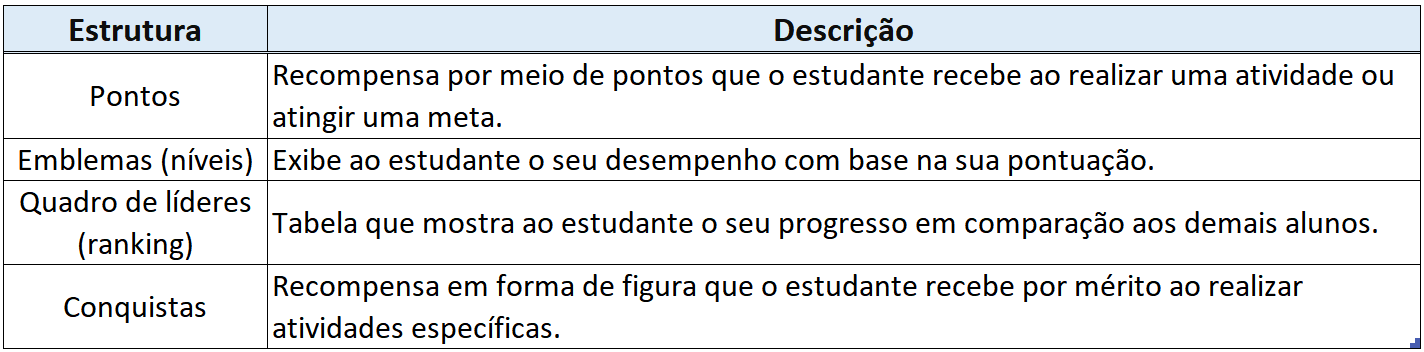
\includegraphics[width=1.0\textwidth]{quadro-04-estrutura-gamificacao.png}
\legend{\footnotesize Fonte: \cite{nicholson2012}. Adaptado pelo Autor}
\label{quad: quadro-04-estrutura-gamificacao}
\end{minipage}
\end{quadro}

Nesse cenário, o desenvolvimento de um jogo sério ou a utilização da gamificação em processos educacionais deve considerar o assunto que será ensinado como base para a criação do sistema de regras, buscando na teoria a ser ensinada as ações e consequências que aparecerão ao longo do jogo e da gamificação. Dessa forma, para alcançar seu potencial, é importante que os jogos sérios e as estratégias de gamificação sejam desenvolvidos de forma a pensar no conteúdo que pretendem ensinar e aplicados em planos de aula planejados para sua utilização.

\chapter{Metodologia da Pesquisa}
A presente pesquisa tem uma abordagem qualitativa ao analisar os dados obtidos, que serão recolhidos por intermédio das respostas dos estudantes nos questionários em anexo. Segundo Minayo (\citeyear{minayo2008}) a pesquisa qualitativa possibilita reorganizar relações, procedimentos, símbolos e acepções da realidade social.

A educação financeira no ensino médio integrado da RFEPCT é algo recente, ainda não estabelecido, o que classifica a pesquisa como exploratória quanto aos objetivos e aplicada em relação à sua natureza. Os estudos bibliográficos originarão um estudo de caso com um pressuposto teórico, que será validado por meio dos procedimentos e objetivos do projeto. Segundo YIN,

\begin{citacao}
Um estudo de caso é uma investigação empírica que investiga um fenômeno contemporâneo dentro de seu contexto da vida real, especialmente quando os limites entre o fenômeno e o contexto não estão claramente definidos \cite{yin2005}.
\end{citacao}

Para atender aos objetivos primários realizou-se uma pesquisa exploratória sobre educação financeira, jogos sérios e simuladores nos projetos pedagógicos dos cursos técnicos integrados nos institutos federais, para verificar a existência do ensino nos campi em todo Brasil; nos principais repositórios de trabalhos acadêmicos, congresso, revistas e cursos voltados para jovens e adolescentes, para identificar as metodologias e práticas de ensino; assim como, nas lojas físicas ou virtuais de aplicativos, \textit{games} e jogos, para encontrar tecnologias que possam ser utilizadas no ensino e aprendizagem da educação financeira para jovens e adolescentes.

Em seguida, considerando o levantamento feito na fundamentação teórica, principalmente nas unidades temáticas, apresentada no capítulo 3, envolvendo conceitos e bases teóricas de educação financeira, elaborou-se planos de aulas separando os conteúdos programáticos de acordo com as unidades temáticas. O quadro \ref{quad: quadro-05-conteudo-programatico} descreve os conteúdos, bem com os objetivos e importância de cada tópico.

\newpage

\graphicspath{{quadros/}}
\begin{quadro}[!ht]
\centering
\begin{minipage}{1.\textwidth}
\caption{Conteúdos Programáticos do Curso}
\centering
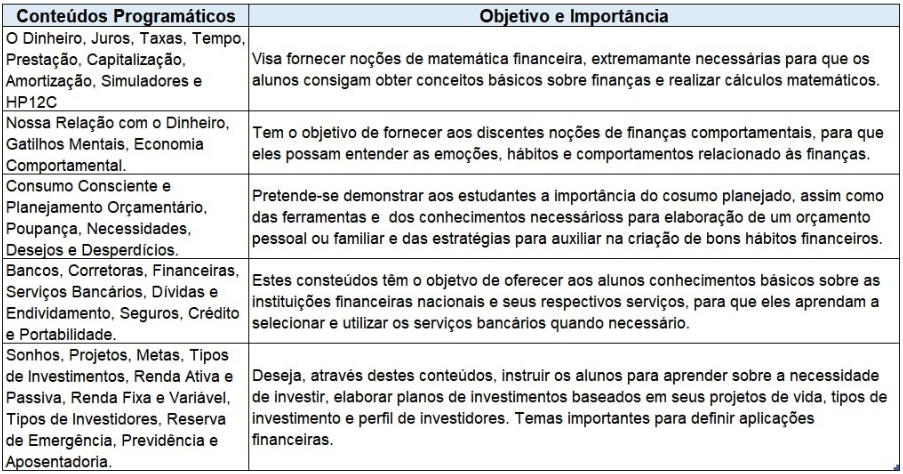
\includegraphics[width=1.0\textwidth]{quadro-05-conteudo-programatico.png}
\legend{\footnotesize Fonte: Dos Autores}
\label{quad: quadro-05-conteudo-programatico}
\end{minipage}
\end{quadro}

Por intermédio de um projeto de ensino, aprovado pela Pró-reitoria de Ensino do IFSUL, foi possível efetivar o presente trabalho realizando a aplicação do plano de aulas em 8 encontros presenciais no curso de Introdução à Educação Financeira para Jovens do ensino médio integrado do IFSUL - Câmpus Gravataí no segundo semestre de 2019, com a participação de 18 alunos e 3 membros ministrantes, especialistas em matemática financeira, contabilidade e investimentos, informática e educação.

A maior parte dos estudantes do curso, 44{\%} destes, possuíam 16 anos, entretanto devido ao fato da pesquisa ser voltada ao ensino médio integral, os alunos que realizaram o curso tinham idades entre 15 a 19 anos. Em relação ao sexo dos discentes 61{\%} eram do masculino e 39{\%} feminino.

A proposta de aplicação do curso foi discutida entre os 3 professores ministrantes, considerando a análise de trabalhos anteriores, referencial teórico, o público-alvo e a experiência dos docentes. Os docentes consideraram que a ordem de apresentação das unidades temáticas que facilitaria o processo de ensino-aprendizagem seria a seguinte:

\begin{enumerate}
    \item Introdução à matemática financeira;
    \item Finanças comportamentais;
    \item Consumo consciente;
    \item Instituições financeiras e serviços;
    \item Investimentos e previdência.
\end{enumerate}

O docente especialista em matemática financeira lecionou a unidade temática de introdução à matemática financeira, o professor especialista em contabilidade e investimentos lecionou a unidade temática referente à investimentos previdência, durante todo o processo de ensino-aprendizagem das duas unidades os ministrantes tiveram assessoria do autor da presente proposta, pesquisador de informática na educação financeira, que também foi responsável por trabalhar as outras unidades temáticas com os discentes.

A infraestrutura necessária para o desenvolvimento desse projeto e execução do plano de ensino nas aulas do curso de Introdução à Educação Financeira para Jovens do ensino médio integrado inclui:

\begin{enumerate}
    \item Material impresso e digital;
    \item Material auxiliar disponibilizado na plataforma \textit{moodle};
    \item Laboratório de informática com acesso à \textit{internet};
    \item Jogos sérios digitais e de tabuleiro;
    \item Projetor multimídia;
    \item Quadro branco.
\end{enumerate}

O conteúdo do curso foi ministrado através de exposições orais seguidas de aulas práticas com atividades no laboratório de informática e/ou trabalhos escritos de cálculos e planejamento, direcionados para a resolução de problemas e exercícios práticos de finanças pessoais e investimentos, visando fixar o conteúdo abordado, com auxílio de tecnologias educacionais como jogos, simuladores e ambientes virtuais de aprendizagem, entre outros. Acredita-se que buscar novas formas de transmitir o conhecimento em sala de aula é relevante, principalmente quando os novos meios de interação que surgem influenciam as formas de pensar e, consequentemente, os estilos de aprendizagem dos estudantes \cite{prensky2012}. Nesse sentido, os jogos sérios podem ser usados no processo de ensino-aprendizagem, pois são desenvolvidos para serem cativantes ao mesmo tempo em que se propõem a alcançar algum objetivo pedagógico.

\section{Os Jogos}
Durante a pesquisa exploratória sobre jogos sérios utilizados no processo de aprendizagem de educação financeira para jovens encontrou-se jogo de tabuleiro como o Desafios Financeiros, \textit{Monopoly}, Banco Imobiliário, Jogo da Vida, Jogo da Mesada, Piquenique, \textit{Cash-flow}, Bons Negócios, Administrando o seu Dinheiro, Catan, Renda Passiva e digitais como o \textit{Cash-flow}, \textit{SimCity}, \textit{The Sims}, \textit{Animal Crossing}, Bate-bola Financeiro, \textit{League of Legends}, \textit{Money Race} 2, Tá O{\$\$}O,  Jogo Vida Financeira, \textit{Tycoon City: New York} e Investindo na Vida.

Foram escolhidos dois jogos para utilizar no curso educação financeira para jovens como apoio à aprendizagem dos discentes, o protótipo Orçamento Consciente e o Renda Passiva. Estes jogos foram escolhidos, pois, permitem ao aluno o aprendizado através de erros e a elaboração de soluções, incentivando-os a resolver problemas de um modo lúdico, refletindo sobre os resultados e sobre o processo de elaboração das soluções, até encontrar um ou mais métodos de soluções possíveis. Ademais, o jogo Orçamento Consciente foi escolhido por trabalhar diretamente com finanças comportamentais e orçamento financeiro. Durante a pesquisa não se encontrou jogos e trabalhos acadêmicos voltados ao ensino de finanças comportamentais em orçamento financeiro para jovens. Por isso, houve a necessidade de desenvolver um protótipo para utilizá-lo no curso, o jogo Orçamento Consciente.

Para mais, normalmente nos jogos de educação financeira do tipo tabuleiro como o \textit{Monopoly}, \textit{Cash-flow} e Banco Imobiliário os jogadores percorrem um caminho semelhante para solucionar os problemas, alcançar os objetivos e ganhar o jogo, dependendo principalmente da sorte para isto. Entretanto, no jogo Renda Passiva, assim como na vida financeira real, não existe um caminho único para solucionar os problemas, alcançar os objetivos e ganhar o jogo, dessa forma o jogo permite aos jogadores elaborar diversas soluções, aprendendo com os próprios erros e assim adquirindo o conhecimento. O Jogo Renda Passiva é um jogo sério de tabuleiro sobre finanças pessoais e familiar, diferente dos jogos tradicionais de tabuleiro onde a sorte é condição principal para ganhar, no Renda Passiva os jogadores deverão desenvolver a capacidade de resolver problemas financeiros para lograr êxito no jogo \cite{frechiani2019a}, de uma forma lúdica, divertida e inteligente pode-se aprender conceitos da educação financeira através do jogo.

Estes fatores foram decisivos na escolha dos jogos utilizados no processo de ensino do curso, contudo é importante descrever motivos para exclusão de outros. Dos existentes excluíram-se os jogos que não permitiam a interação entre os alunos, que o fator de sorte é componente decisivo, que trabalham com poucos conteúdos das unidades temáticas, que lidam apenas com perguntas e respostas, que o público-alvo são crianças e com custo elevado para aquisição, pois nem sempre a instituição de ensino possui recursos para compra de jogos, deste modo quanto menor o custo relacionado melhor. Os aspectos inerentes aos jogos escolhidos, bem como o uso destes nos processos educativos estão descritos neste capítulo nos próximos itens.

\subsection{O Jogo Orçamento Consciente}
O jogo Orçamento Consciente é um protótipo de um jogo sério digital, disponível para computadores e \textit{smartphones}, desenvolvido em 2018 pelos alunos Camila Peres, Johnata Santicioli (autor da presente proposta) e Willian Chimura do Mestrado Profissional em Informática na Educação no Instituto Federal do Rio Grande do Sul.

O jogo simula o recebimento de um salário mensal de R{\$}3.000,00 que deve ser dividido em três necessidades: compras e conforto, alimentação e saúde nesta ordem da esquerda à direita conforme a Figura \ref{fig: figura01-salario}, neste momento inicial ilustrado na figura, o jogador realiza um orçamento financeiro mesmo que de forma aleatória, após distribuir todo o salário do mês o jogo apresenta uma contagem regressiva para início do jogo, Figura \ref{fig: figura02-contagem}.

\graphicspath{{figuras/}}
\begin{figure}[!ht]
\centering
\begin{minipage}{1.\linewidth}
\center
\caption{Jogo Orçamento Consciente (Distribuição do Salário)} \label{fig: figura01-salario}
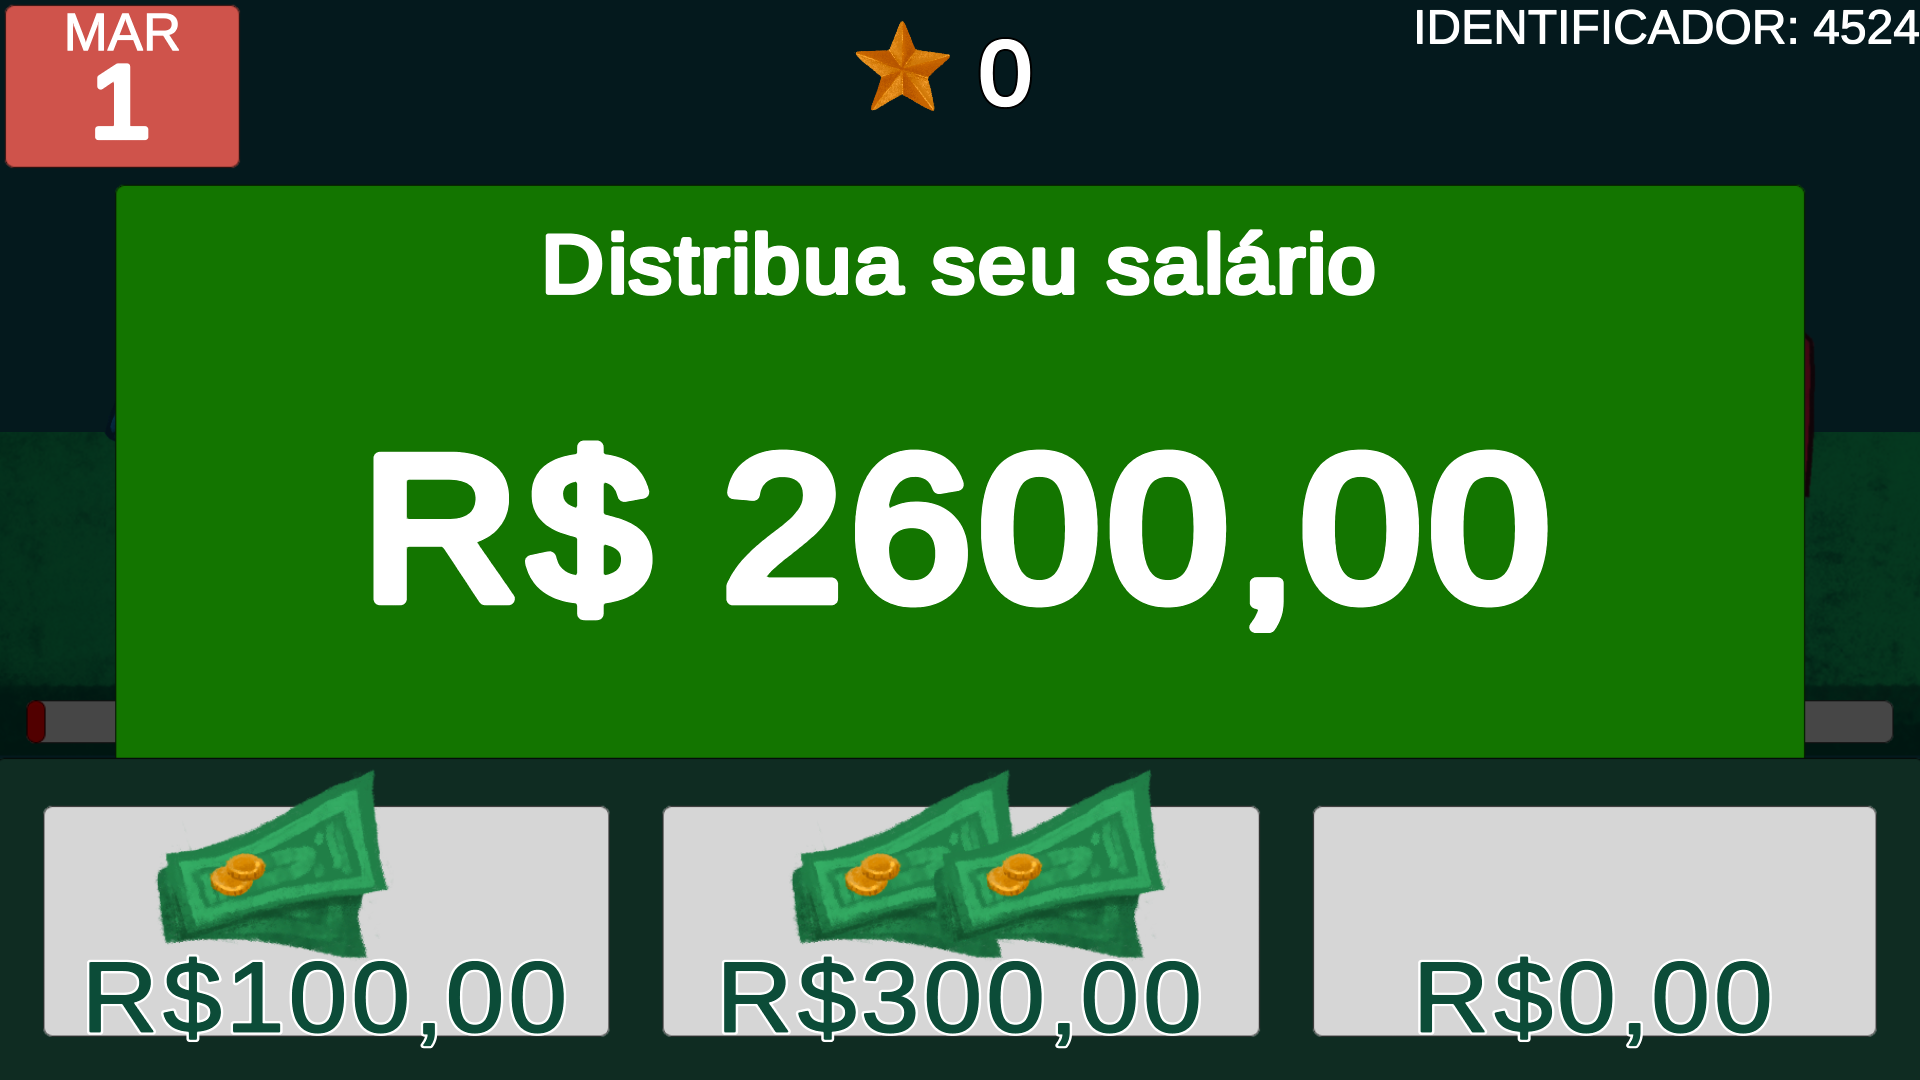
\includegraphics[width=0.4\linewidth]{01-figura_distribuicao-salario.png}
\legend{\footnotesize Fonte: Dos Autores}
\end{minipage}
\end{figure}

\graphicspath{{figuras/}}
\begin{figure}[!ht]
\centering
\begin{minipage}{1.\linewidth}
\center
\caption{Jogo Orçamento Consciente (Contagem Regressiva)} \label{fig: figura02-contagem}
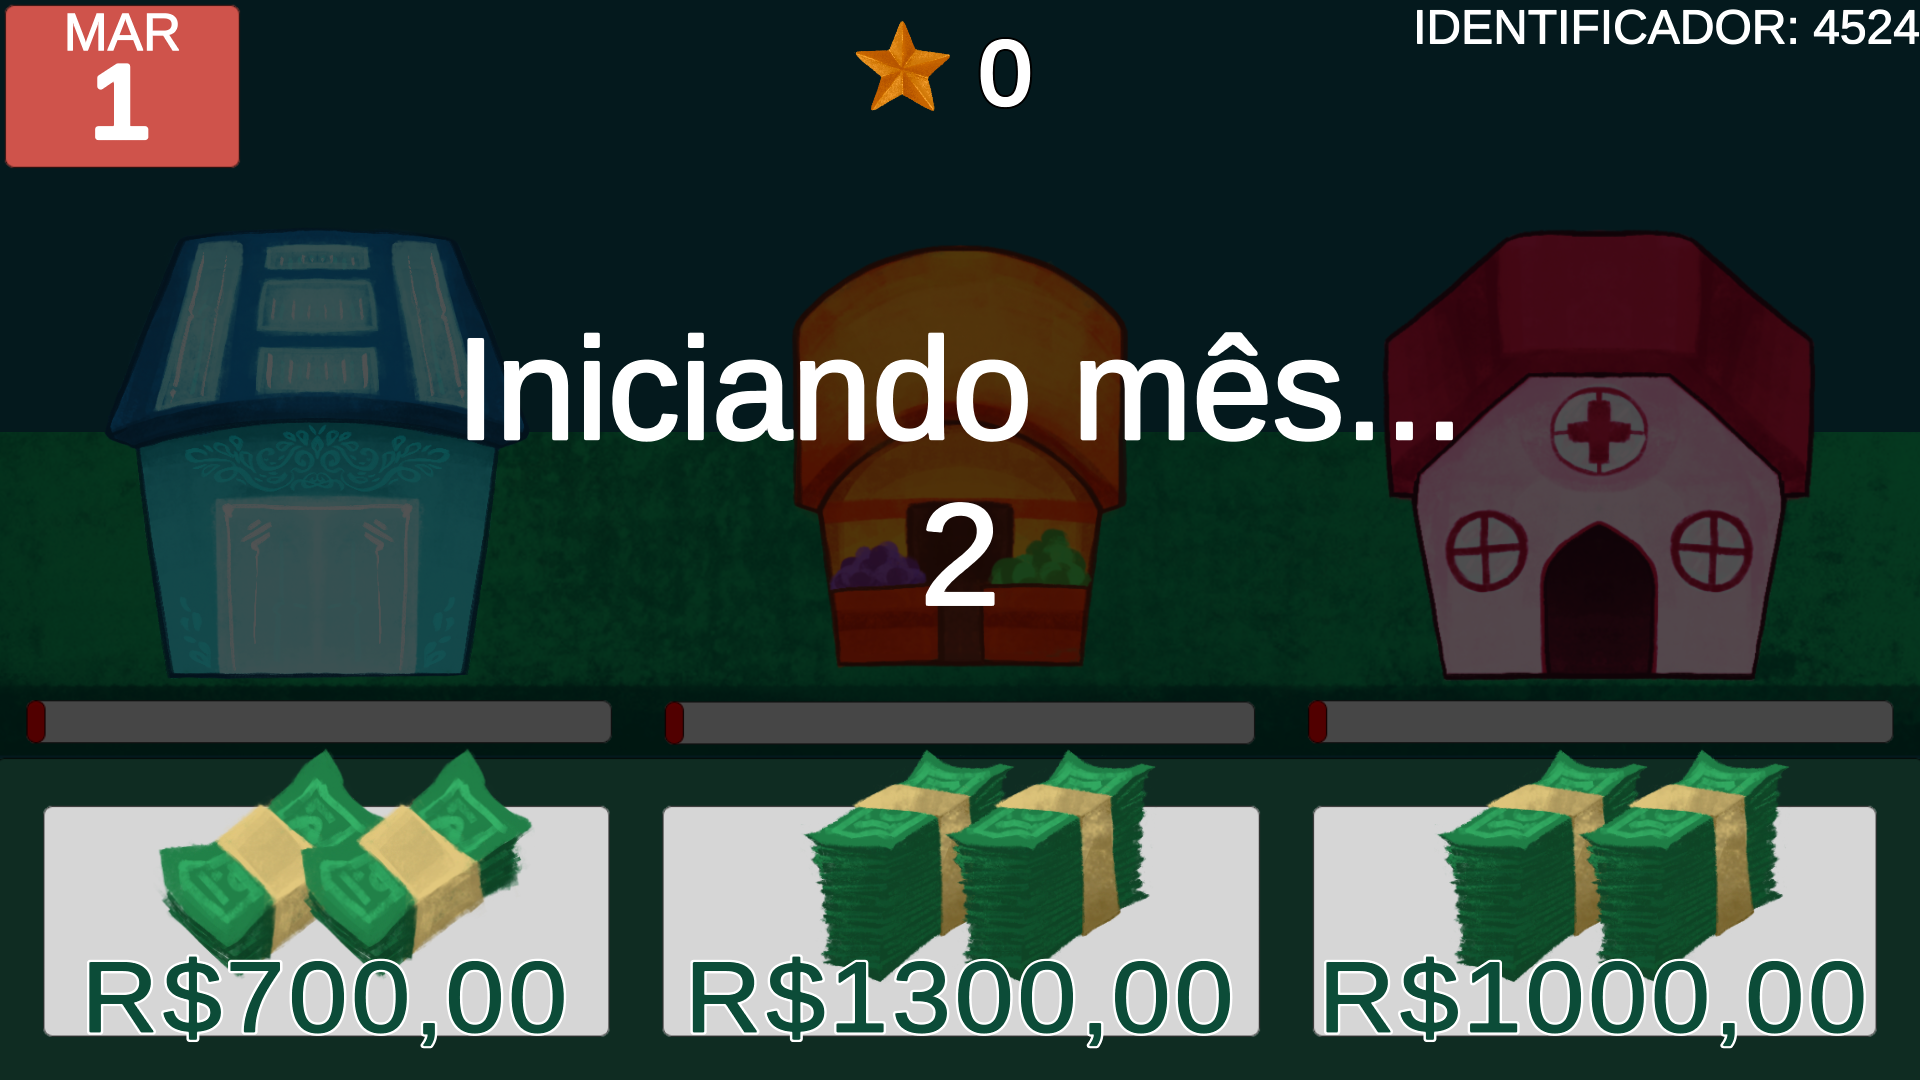
\includegraphics[width=0.4\linewidth]{02-figura_contagem-regressiva-mes.png}
\legend{\footnotesize Fonte: Dos Autores}
\end{minipage}
\end{figure}

Ao longo de “um mês”, que dentro do jogo dura aproximadamente 1 minuto, o jogador deve equilibrar suas necessidades, escolhendo quais produtos comprar e quais ignorar, considerando o custo-benefício e seu planejamento inicial (Figura \ref{fig: figura03-mercado} e \ref{fig: figura04-shopping}), podendo apenas utilizar o dinheiro da necessidade com o respectivo produto, em outras palavras, utilizar o dinheiro reservado para saúde apenas com produtos de saúde. O jogador não pode transferir dinheiro de uma necessidade para outra, ao esgotar os recursos destinados para determinada necessidade, o jogador precisa esperar até o mês seguinte para repensar sua estratégia e ajustar o planejamento orçamentário para torná-lo superavitário ou neutro.

\graphicspath{{figuras/}}
\begin{figure}[!ht]
\centering
\begin{minipage}{1\linewidth}
\centering
\caption{Jogo Orçamento Consciente (Produto Mercado)} \label{fig: figura03-mercado}
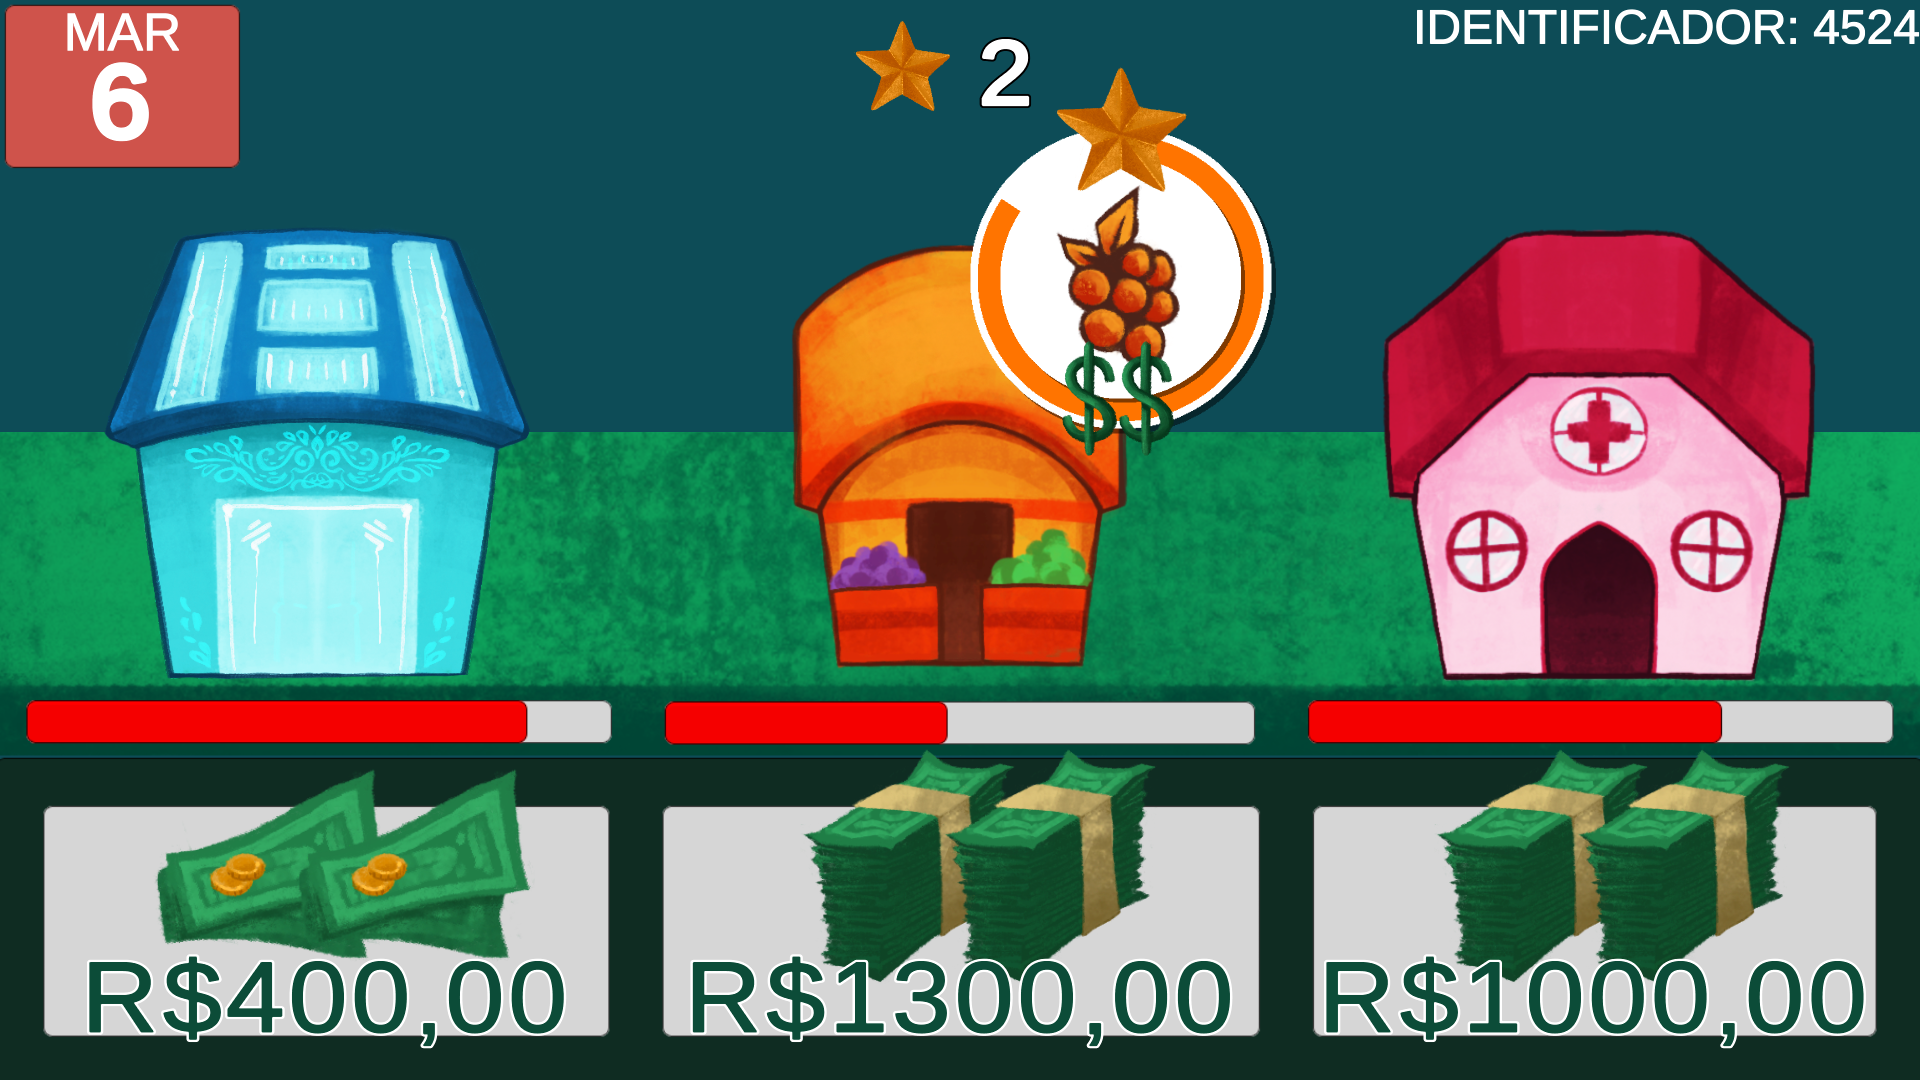
\includegraphics[width=0.4\linewidth]{03-figura_tela-jogo-mercado.png}
\legend{\footnotesize Fonte: Dos Autores}
\end{minipage}
\end{figure}

\graphicspath{{figuras/}}
\begin{figure}[!ht]
\centering
\begin{minipage}{1\linewidth}
\centering
\caption{Jogo Orçamento Consciente (Produto Shopping)} \label{fig: figura04-shopping}
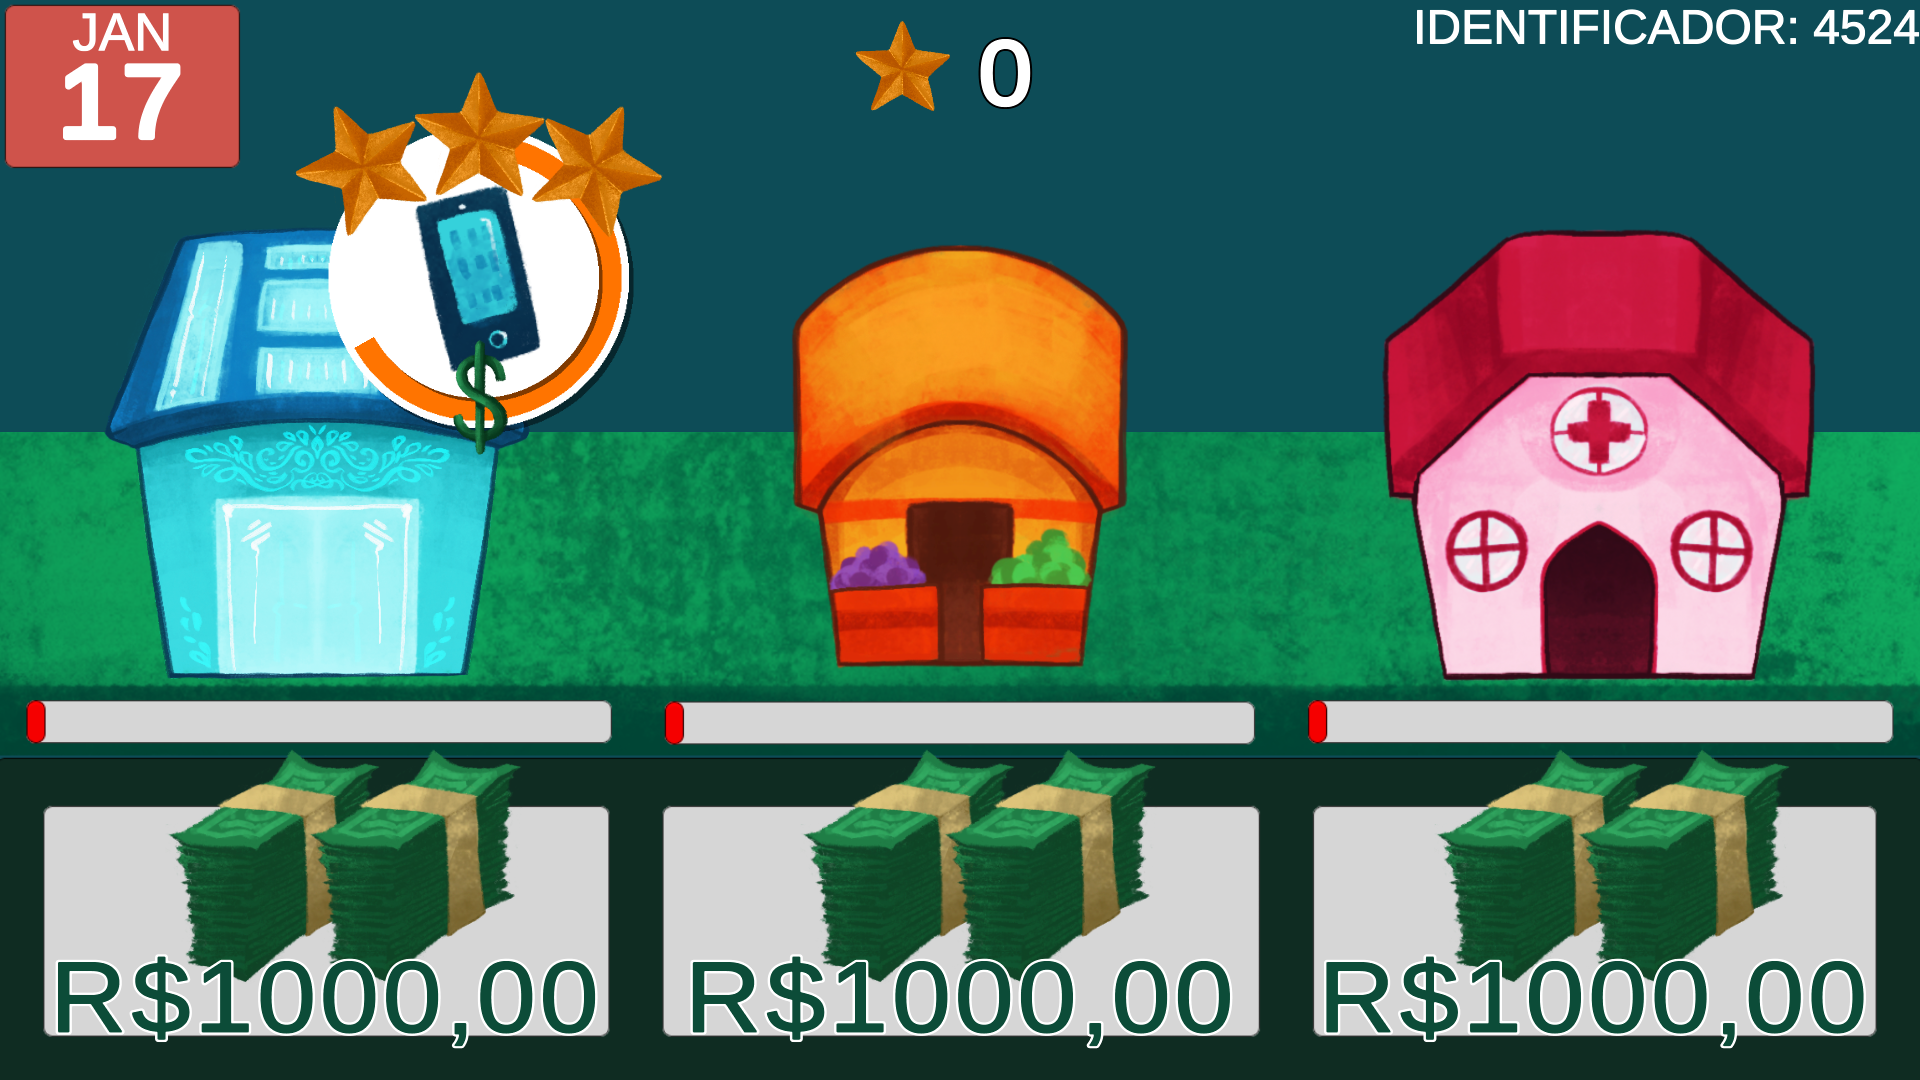
\includegraphics[width=0.4\linewidth]{04-figura_tela-jogo-shopping.png}
\legend{\footnotesize Fonte: Dos Autores}
\end{minipage}
\end{figure}

\newpage
A tela principal do jogo, exibidas nas Figuras \ref{fig: figura03-mercado} e \ref{fig: figura04-shopping}, apresenta três “prédios" (construções do jogo), um azul que representa um shopping, relacionado à “necessidade de compras e conforto”, um mercado na cor laranja, que corresponde a “necessidade de comida” e uma farmácia rosa simbolizando a “necessidade de remédios ou saúde”. As barras horizontais vermelhas (“barras de necessidade”) embaixo de cada construção indicam ao jogador a necessidade de consumir produtos de acordo com sua categoria. Essas barras iniciam totalmente preenchidas (necessidade de consumo atendida) e diminuem conforme o tempo do jogo, representando o dever de uma nova compra. Abaixo de cada uma das barras encontra-se a quantidade de dinheiro distribuída no começo de cada mês do jogo e disponível para o consumo da respectiva necessidade.

Cada “prédio” oferece opções de produtos relativos à necessidade que representa, um após o outro, cabendo ao jogador a decisão de comprar ou não os produtos disponíveis. Para efetuar a compra o jogador deve selecionar o produto, considerando o planejamento orçamentário realizado, se o item é necessário e se é viável a sua aquisição. Cada produto possui diferentes níveis de qualidade, representados por estrelas (de uma a três), bem como diferentes preços, representados por cifrões (de uma a três), cada um equivale a cem reais. Quanto maior a qualidade do produto, maior será a quantidade de estrelas e supre mais a necessidade de consumo, aumentando o preenchimento da barra vermelha que indica a necessidade. Por exemplo, a Figura \ref{fig: figura03-mercado} ilustra um item que pode ser comprado pelo o jogador junto ao prédio do supermercado, um cacho uva que possui qualidade nível 1, pois tem uma estrela, e preço de R{\$} 200 (duzentos reais), porque há 2 (dois) cifrões. Cada item comprado faz com que o orçamento planejado sofra alterações, diminuindo os recursos para a aquisição de itens de uma mesma categoria. Os produtos ficam disponíveis para compra por um determinado tempo, controlado pelo círculo laranja em volta do produto, quando o círculo completa uma volta o tempo para comprar o produto acaba (uso dos Gatilhos Mentais da Urgência e Escassez) e então desaparece e eventualmente são substituídos por outros, com diferentes qualidades e preços. Nas figuras \ref{fig: figura03-mercado} e \ref{fig: figura04-shopping}, acima das construções existe um contador de estrelas, referente à qualidade do produto. Ao comprar produtos de maior qualidade essa pontuação aumenta conforme a quantidade de estrelas do produto, ao esvaziar completamente a barra de necessidade, essa ficará cinza, pois não houve consumo suficiente. Cabe ao jogador escolher quais produtos comprar, baseando-se em seu planejamento inicial, preço, qualidade e necessidade.

Ao final do mês o jogador recebe um relatório detalhando as necessidades que foram atendidas ou não e sua pontuação (Figuras \ref{fig: figura05-relatorio-01} e \ref{fig: figura06-relatorio-02}), a cada dia que uma das barras de necessidade estiver totalmente vazia é descontada uma estrela do total, em caso de sobra de recursos, cada R{\$} 100 é convertido em uma estrela. Por exemplo, na Figura \ref{fig: figura06-relatorio-02}, o relatório mês indica que o jogador passou 4 dias sem recurso no Shopping, 3 dias sem recursos no Mercado e poupou com R{\$} 500 de seu salário, com isso duas estrelas serão retiradas das 56 que ele possui.

\graphicspath{{figuras/}}
\begin{figure}[!ht]
\centering
\begin{minipage}{1\linewidth}
\center
\caption{Jogo Orçamento Consciente (Tela de Relatório Mês 1)} \label{fig: figura05-relatorio-01}
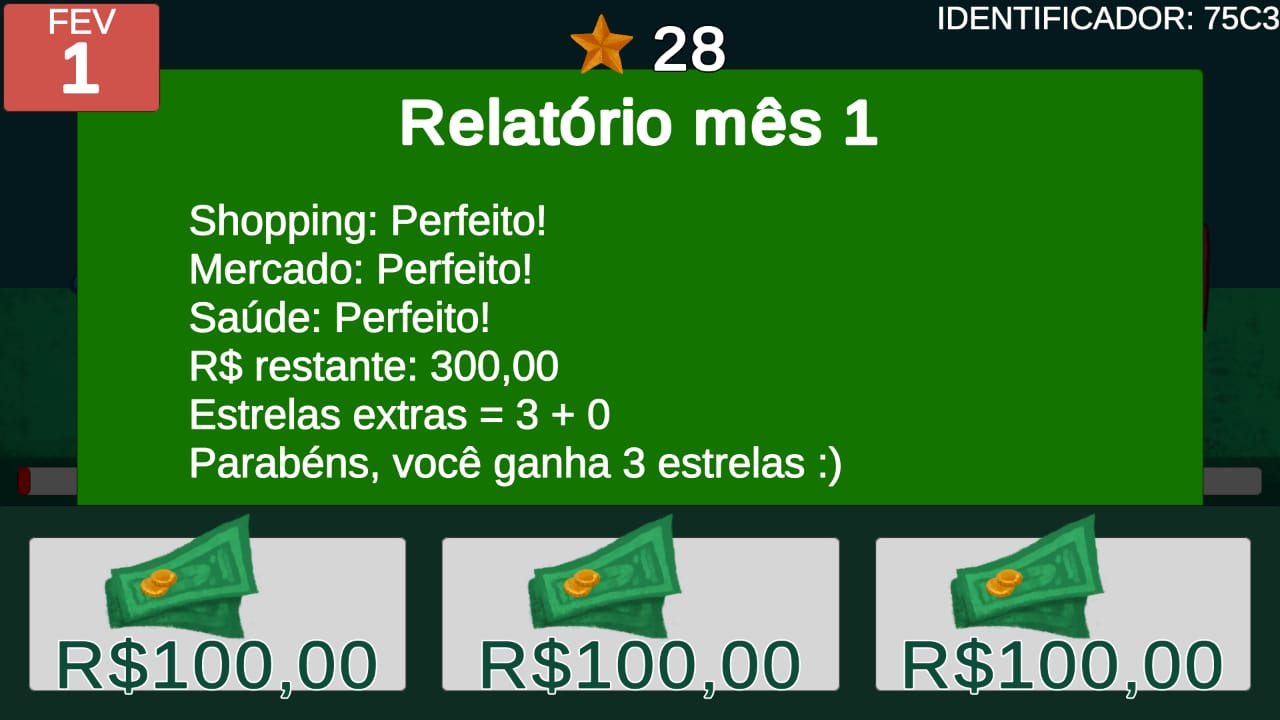
\includegraphics[width=0.4\linewidth]{05-figura_relatorio-mes-1}
\legend{\footnotesize Fonte: Dos Autores}
\end{minipage}
\end{figure}

\graphicspath{{figuras/}}
\begin{figure}[!ht]
\centering
\begin{minipage}{1\linewidth}
\center
\caption{Jogo Orçamento Consciente (Tela de Relatório Mês 2)} \label{fig: figura06-relatorio-02}
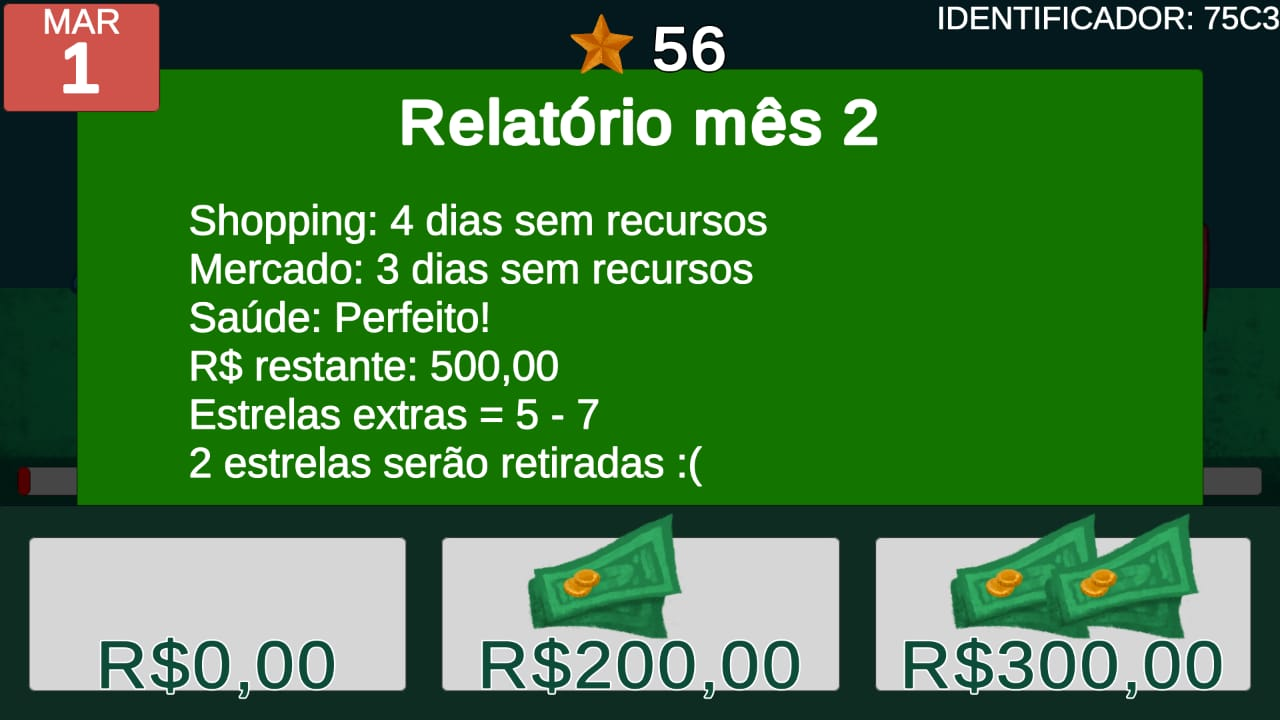
\includegraphics[width=0.4\linewidth]{06-figura_tela-relatorio-mes-2}
\legend{\footnotesize Fonte: Dos Autores}
\end{minipage}
\end{figure}

Dessa forma, o jogo permite aos alunos a possibilidade de testar os conhecimentos teóricos em uma simulação simples, podendo ver as consequências de suas ações de forma rápida em um ambiente seguro.

\subsection{O Jogo Renda Passiva}
O jogo Renda Passiva, desenvolvido por Daniel Frechiani, simula a vida financeira pessoal e familiar, por meio de um personagem no jogo, podendo o jogador escolher o personagem entre um microempresário, servidor público, empresário, motorista de aplicativo, professora e advogada. Todos os personagens possuem receitas (salário ou pró-labore), gastos (fixos, variáveis, impostos, seguros, financiamento, cartão de crédito e diversos), dívidas e podem obter no decorrer do jogo ativos (ações e títulos de renda fixa) conquistando assim uma renda passiva. O controle e anotações destes itens devem ser feitos através da ficha financeira, apresentada na Figura \ref{fig: figura07-ficha-financeira}. Além das fichas financeiras o jogo possui cartas para obter negócios, imóveis, renda fixa, ofertas e ações, e também, cartas surpresas, dados para percorrer as casas, pinos que representam os jogadores, canetas e apagadores para atualizar as fichas financeiras.

\graphicspath{{figuras/}}
\begin{figure}[!ht]
\centering
\begin{minipage}{1.\textwidth}
\caption{Jogo Renda Passiva (Ficha Financeira)}
\centering
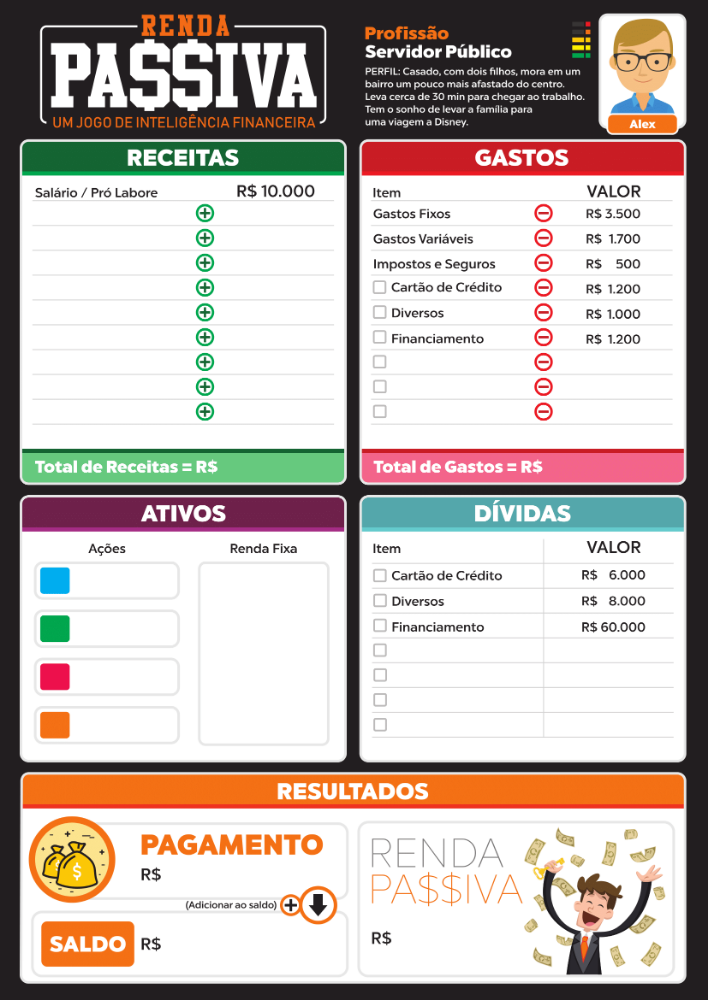
\includegraphics[width=0.45\textwidth]{07-figura_ficha-financeira-renda-passiva}
\legend{\footnotesize Fonte: Frechiane, Manual do Jogo (\citeyear{frechiani2019b})}
\label{fig: figura07-ficha-financeira}
\end{minipage}
\end{figure}

Ao iniciar o jogo os jogadores percorrem tabuleiro (Figura \ref{fig: figura08-tabuleiro}) e precisam passar pelos ícones de sacos de dinheiros para receberem pagamentos (já com os gastos descontados).

\graphicspath{{figuras/}}
\begin{figure}[!ht]
\centering
\begin{minipage}{1.\textwidth}
\caption{Jogo Renda Passiva (Tabuleiro do Jogo)}
\centering
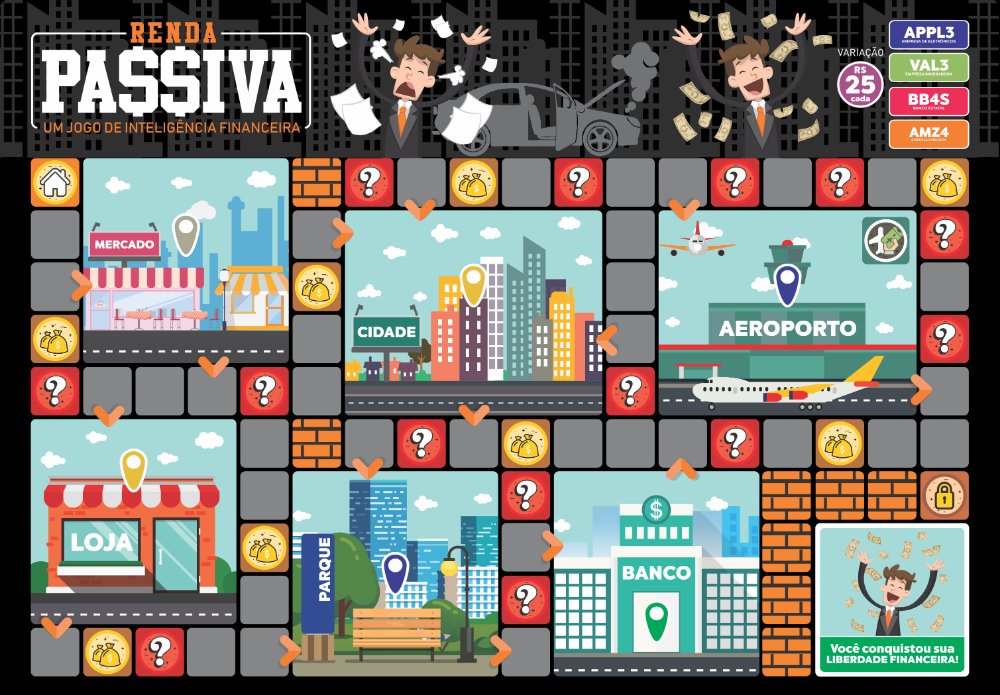
\includegraphics[width=0.5\textwidth]{08-figura_tabuleiro-renda-passiva}
\legend{\footnotesize Fonte: Frechiane, Manual do Jogo (\citeyear{frechiani2019b})}
\label{fig: figura08-tabuleiro}
\end{minipage}
\end{figure}

\newpage
Diferente da maior parte dos jogos sobre finanças que possui um caminho único, neste o jogador pode decidir por qual caminho seguir no tabuleiro de acordo com o planejamento que possui e assim determinar uma estratégia de jogo, sendo capaz de decidir entre quitar as dívidas, investir em ações, renda fixa, comprar imóveis ou negócios, considerando o risco, a liquidez e a rentabilidade de cada um. Para isso basta apenas movimentar-se para os respectivos cenários (Figura \ref{fig: figura09-cenario-jogo}) e retirar uma carta, exceto as cartas ações que podem ser solicitadas em qualquer posição do tabuleiro na vez de cada jogador. Dessa forma, o jogo proporciona ao jogador tentar construir diversas soluções possíveis para cada problema proposto pelo jogo. A cada nova solução concebida, aumenta a compreensão dos alunos a respeito do processo de solução dos problemas financeiros propostos pelo jogo.

\graphicspath{{figuras/}}
\begin{figure}[!ht]
\centering
\begin{minipage}{1.\textwidth}
\caption{Jogo Renda Passiva (Cenários do Jogo)}
\centering
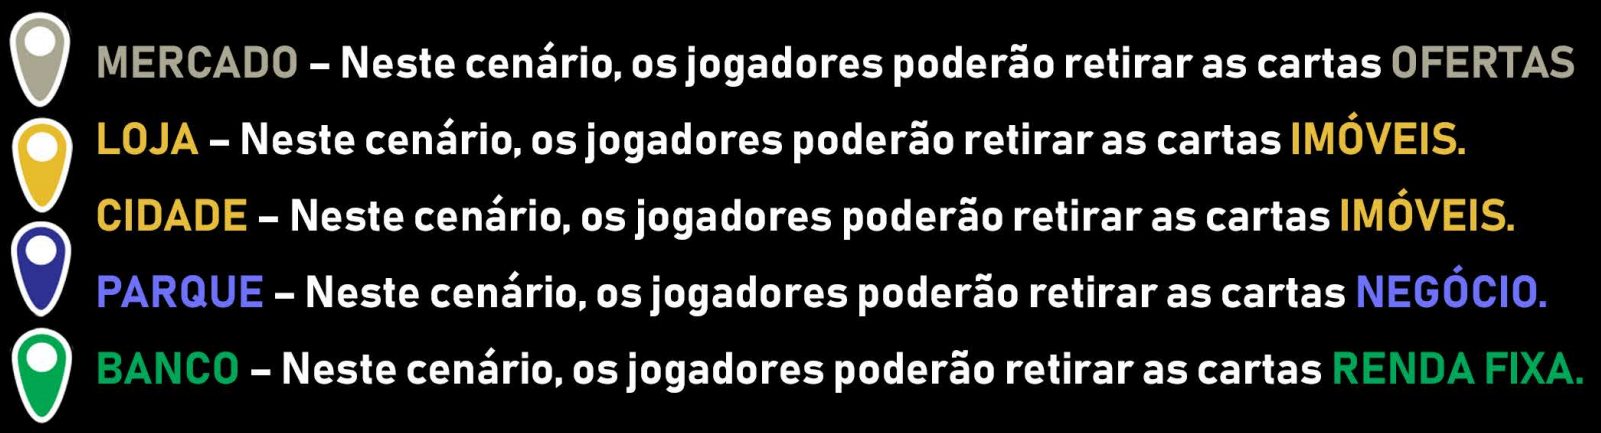
\includegraphics[width=0.8\textwidth]{09-figura_cenario-jogo-renda-passiva}
\legend{\footnotesize Fonte: Frechiane, Manual do Jogo (\citeyear{frechiani2019b})}
\label{fig: figura09-cenario-jogo}
\end{minipage}
\end{figure}

Nas cartas surpresa o jogador pode encontrar riscos e oportunidades como: demissão, crise econômica, adição de um novo filho à família (aumentando o gasto), 13º Salário, promoção no trabalho, recebimento de dividendos entre outros.

O jogador que conseguir cumprir os 3 objetivos do jogo: quitar todas as dívidas, ter uma renda passiva igual ou maior ao seu total de gastos, chegar ao cenário da conquista (casa com cadeado), vence o jogo.

\section{A Avaliação}
Análise dos dados da presente pesquisa está sendo executada por intermédio de uma abordagem qualitativa, com o objetivo de verificar se a metodologia adotada no decorrer do curso de Introdução à Educação Financeira para Jovens contribuíram no processo de aprendizagem, bem como aferir o nível retenção dos temas principais apresentados, conhecimento prévio, motivação para participar do curso, interesse em buscar novos conhecimentos, a disseminação do conhecimento adquirido e a consciência da importância do tema.

Os dados foram coletados através de formulários virtuais na derradeira etapa do curso, exceto os para avaliar a experiência dos alunos e sua percepção de aprendizagem em relação ao jogo sério, coletados logo após a utilização dos jogos. As informações obtidas por meio do Questionário de Avaliação da Aprendizagem (Apêndice \ref{apend-a}) para aferir o nível de retenção do conteúdo apresentado durante o curso; Questionário de Avaliação do Curso (Apêndice \ref{apend-b}) para verificar o conhecimento prévio, a motivação para participar do curso, o interesse em buscar novos conhecimentos, a disseminação do conhecimento adquirido e a consciência da importância do tema pelos estudantes; e pelo método avaliativo MEEGA+ (\textit{Model for Evaluating Educational Games}) para avaliar a experiência e a percepção de aprendizagem dos alunos.

O método MEEGA+ possui um questionário para avaliar a experiência subjetiva do jogador, permitindo a coleta de dados sobre aspectos como o foco da atenção, diversão, desafio, interações sociais, relevância, satisfação, usabilidade e percepção de aprendizagem (PETRI, \citeyear{petri2017}), também apresenta uma seção para relatar pontos fortes, fracos e comentários adicionais. Este método busca agir de forma rápida e não intrusiva para maior efetividade em avaliar a qualidade dos jogos.

Os dados coletados no retorno dos questionários respondido pelos alunos, possibilitarão aos pesquisadores categorizar e analisar as respostas no intuito de verificar quais objetivos propostos foram atingidos e a verificar a confirmação ou não da hipótese. Ao refletir sobre os dados coletados, espera-se chegar à conclusão sobre a potencialidade que o curso, bem como a metodologia utilizada e os jogo possibilitam para aquisição do conhecimento relativo aos conteúdos abordados.

\chapter{Produto: Curso de Introdução à Educação Financeira para Jovens do Ensino Médio}
Conforme citado em seções anteriores, o produto desta pesquisa é o curso de Introdução à Educação Financeira para Jovens do ensino médio integrado, voltado principalmente para os institutos federais e outras autarquias da RFEPCT. Com base nos resultados, sugestões e as propostas de trabalhos diretamente relacionados ao tema pesquisado foi possível estabelecer 5 unidades temáticas abordadas no curso: matemática financeira, finanças comportamentais, consumo consciente, instituições financeiras e serviços, investimentos e previdência.

O conteúdo abordado no curso é ministrado em 8 encontros com 2 aulas de 45 minutos cada, o quadro \ref{quad: quadro-06-tema-e-conteudo} elenca em conjunto das unidades temáticas os respectivos conteúdos programáticos. O objetivo instrucional, conhecimento prévio, recursos utilizados, tema e desenvolvimento de cada encontro são descritos no decorrer deste capítulo.

\graphicspath{{quadros/}} 
\begin{quadro}[!ht]
\centering
\begin{minipage}{1.\textwidth}
\caption{Unidade Temáticas e Conteúdos Programáticos do Curso}
\centering
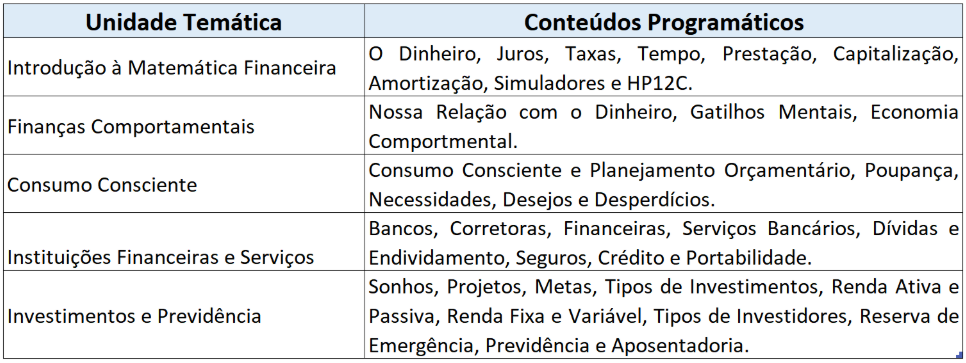
\includegraphics[width=1.0\textwidth]{quadro-06-tema-e-conteudo.png}
\legend{\footnotesize Fonte: O autor, 2019}
\label{quad: quadro-06-tema-e-conteudo}
\end{minipage}
\end{quadro}

\section{1º Encontro - Matemática Financeira}
Quando possível, o primeiro encontro deve ser ministrado por um docente especialista em matemática financeira e educação, pois este, teoricamente, detém um domínio amplo sobre matemática financeira. Partindo do princípio que os alunos têm conhecimento básico sobre o Sistema Monetário Brasileiro para efetuar contratação de serviço ou compra de produto, aprendizado este adquirido nos anos iniciais do ensino fundamental e na vivência do aluno, o quadro \ref{quad: quadro-07_plano-aula-1} apresenta o plano de aula do 1º encontro no qual é abordado especificamente a unidade temática introdução à matemática financeira.

\newpage

\graphicspath{{quadros/}}
\begin{quadro}[!ht]
\centering
\begin{minipage}{1.\textwidth}
\caption{Plano de Aula 1º Encontro do Curso}
\centering
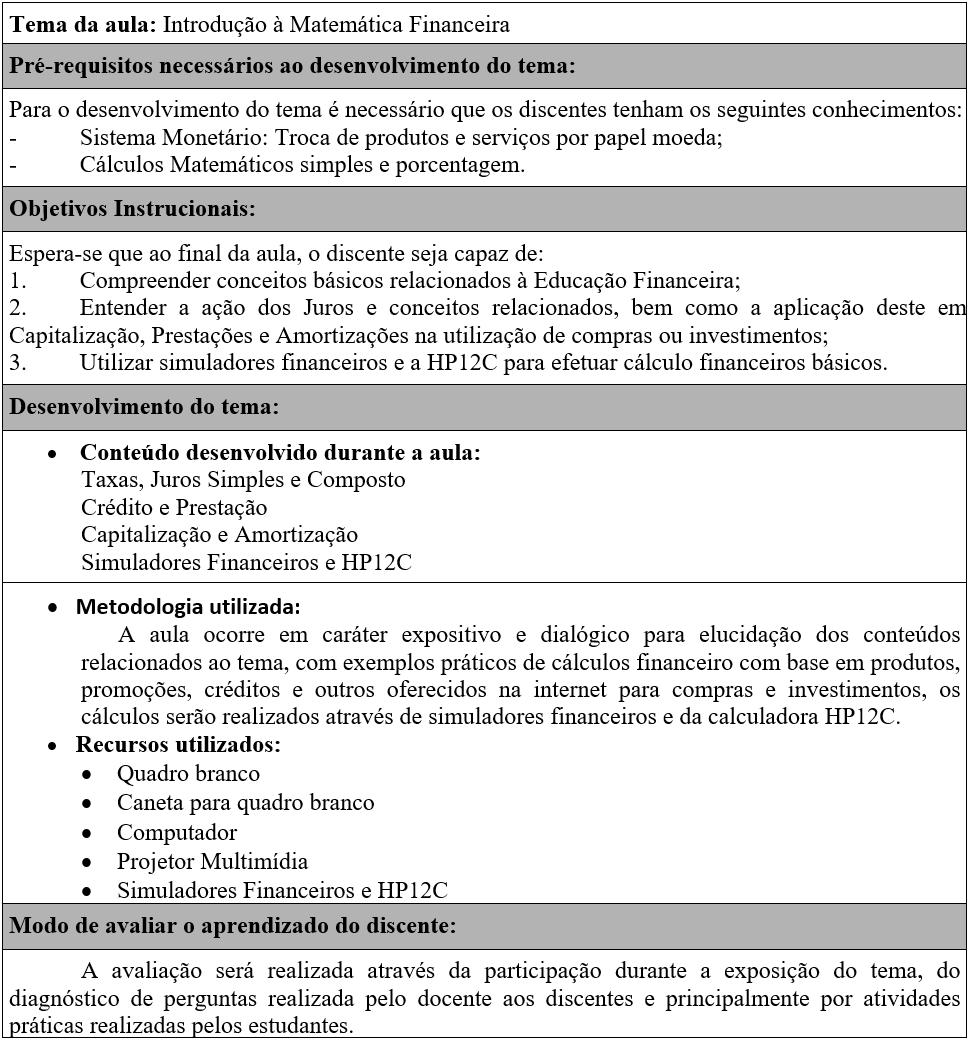
\includegraphics[width=0.9\textwidth]{quadro-07_plano-aula-1.png}
\legend{\footnotesize Fonte: O autor, 2019}
\label{quad: quadro-07_plano-aula-1}
\end{minipage}
\end{quadro}

Para realizar os cálculos financeiros durante a aula, são utilizados exemplos de produtos os quais os façam parte do conhecimento dos discentes para tornar o processo de aprendizagem interessante e engajante.

\section{2º Encontro - Finanças Comportamentais}
No segundo encontro é exposto aos discentes a unidade temática referente à introdução às Finanças Comportamentais. Os conteúdos e os objetivos da aula temática estão descritos no plano de aula do 2º encontro e são apresentados no quadro \ref{quad: quadro-08_plano-aula-2}.

\newpage

\graphicspath{{quadros/}} 
\begin{quadro}[!ht]
\centering
\begin{minipage}{1.\textwidth}
\caption{Plano de Aula 2º Encontro do Curso}
\centering
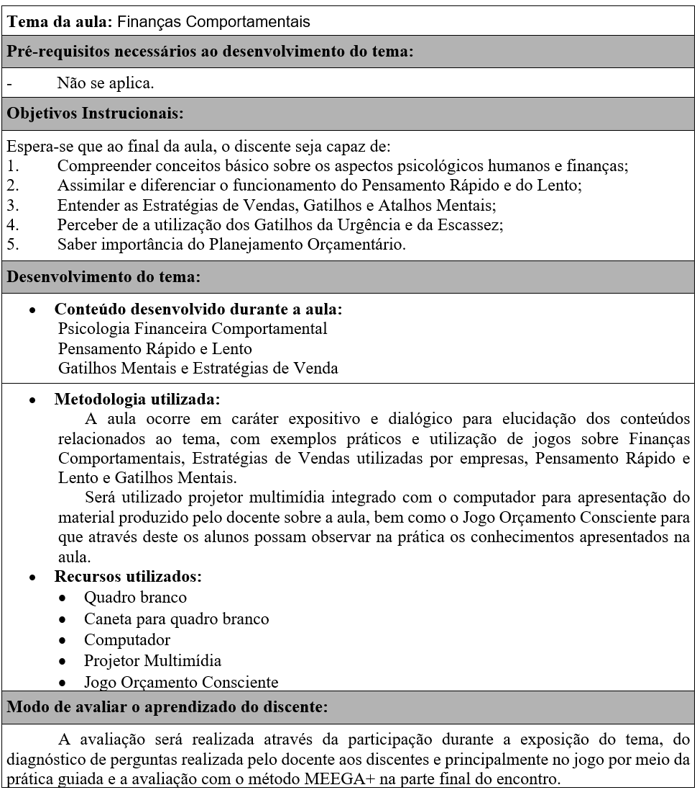
\includegraphics[width=0.9\textwidth]{quadro-08_plano-aula-2.PNG}
\legend{\footnotesize Fonte: O autor, 2019}
\label{quad: quadro-08_plano-aula-2}
\end{minipage}
\end{quadro}

O jogo sério foi utilizado por intermédio do computador onde cada discente interage individualmente com o \textit{game}, desta forma pode-se observar, associar e obter melhor compreensão sobre os temas abordados em aula. No final da aula é aplicado uma avaliação do jogo por intermédio do método MEEGA+.

Estruturou-se a presente aula para auxiliar no processo de ensino e aprendizagem, bem como no desenvolvimento cognitivo do estudante, para que este inicie a transição do estágio Consumidor Sensorial (consumo baseado em sensações) para o Consumidor Pré-Poupador (consumo consciente dos recursos financeiros), assim como assimilar a importância do planejamento orçamentário.

\section{3º Encontro - Consumo Consciente}
Após os discentes entenderem a importância de planejar seus gastos, a unidade temática do terceiro encontro apresenta o Consumo Consciente relacionado às finanças, que possui o intuito de demonstrar como executar o planejamento orçamentário. Os conteúdos relacionados à unidade temática estão elencados no quadro \ref{quad: quadro-09_plano-aula-3} que apresenta o plano de aula do 3º encontro.

\graphicspath{{quadros/}} 
\begin{quadro}[!ht]
\centering
\begin{minipage}{1.\textwidth}
\caption{Plano de Aula 3º Encontro do Curso}
\centering
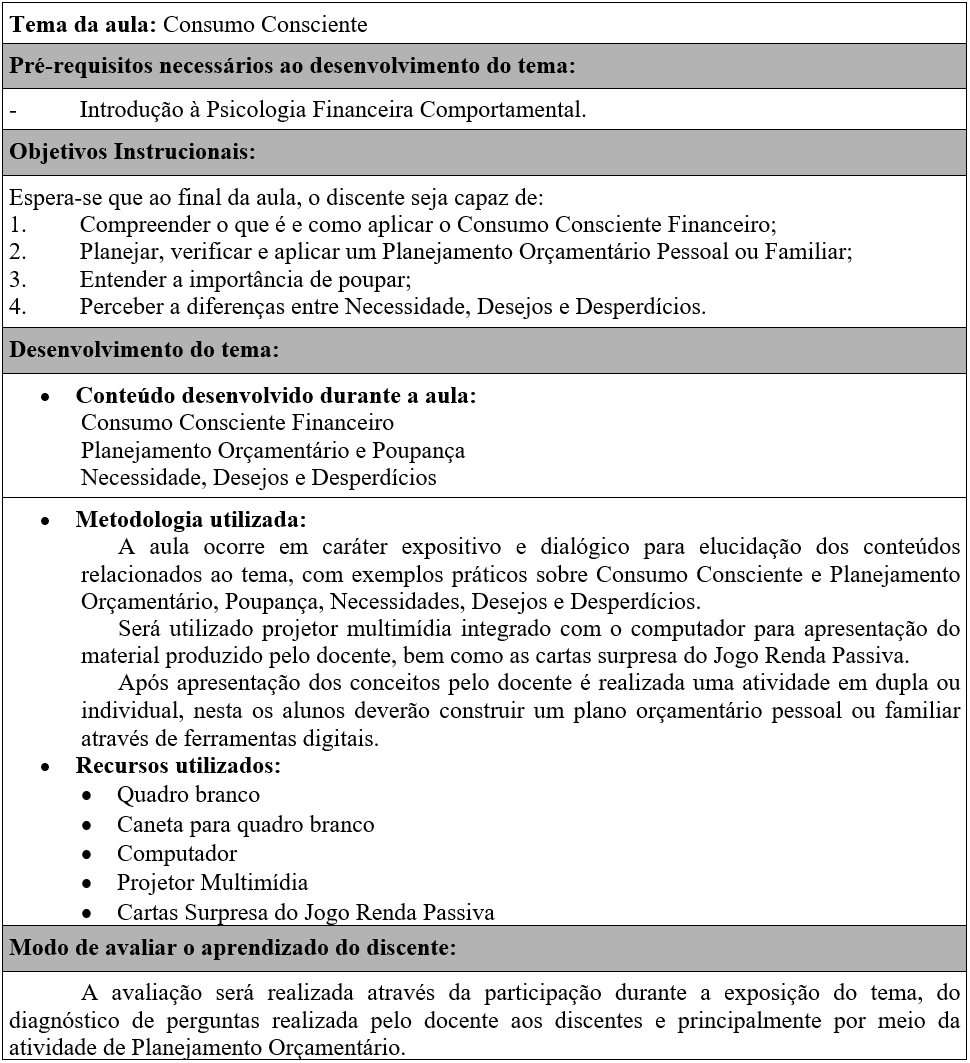
\includegraphics[width=0.9\textwidth]{quadro-09_plano-aula-3}
\legend{\footnotesize Fonte: O autor, 2019}
\label{quad: quadro-09_plano-aula-3}
\end{minipage}
\end{quadro}

Após apresentação do conteúdo os discente realizam a atividade de planejamento orçamentário, individual (Pessoal) ou em dupla (Familiar), na qual definirão uma profissão que almejam trabalhar, buscar o salário médio respectivo e defini-lo como receita, o plano deve conter despesas com habitação (aluguel e condomínio), saúde, transporte, educação, contas residenciais e alimentação, o professor define um valor por pessoa por cada categoria de gastos.

Os alunos deverão poupar valores em seus planos e retirar uma carta surpresa do jogo Renda Passiva que influenciará no orçamento. As cartas surpresa do jogo contêm oportunidades (restituição de imposto, bônus da empresa, promoção no trabalho etc.), riscos (multas de trânsito, demissão, imposto etc.) entre outros como a chegada de um filho que aumenta a despesa em 10{\%} do salário (Figura \ref{fig: figura-10-carta-surpresa}).

\graphicspath{{figuras/}} 
\begin{figure}[!ht]
\centering
\begin{minipage}{1.\textwidth}
\caption{Jogo Renda Passiva (Carta Surpresa)}
\centering
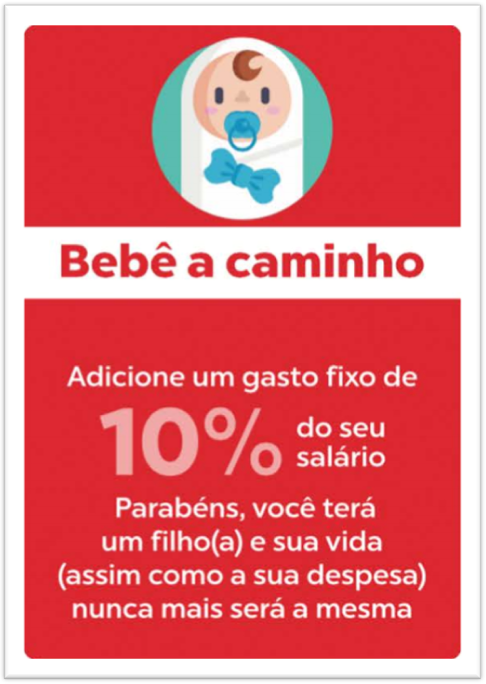
\includegraphics[width=0.3\textwidth]{10-figura_carta-surpresa-renda-passiva}
\legend{\footnotesize Fonte: Frechiane (\citeyear{frechiani2019b})}
\label{fig: figura-10-carta-surpresa}
\end{minipage}
\end{figure}

Ao aplicar o conhecimento adquirido nessa aula em sua vida, o aluno alcança o estágio \textbf{Consumidor Pré-Poupador} do desenvolvimento cognitivo financeiro, consumindo de forma consciente com planos de aquisição de produto e serviços estabelecidos anteriormente, diminuindo o impacto das estratégias de vendas e gatilhos mentais sem suas decisões de compras.

\section{4º Encontro - Instituições Financeiras}
O objetivo do quarto encontro é explanar aos estudantes os tipos de instituições financeiras (bancos, corretoras de investimento, seguradoras e financeiras) e seus respectivos serviços (cesta de serviço, seguros, investimentos, crédito e portabilidade), bem como sobre dívidas e endividamentos. Os conteúdos relacionados a unidade temática estão descritos no quadro \ref{quad: quadro-10_plano-aula-4} que apresenta o plano de aula do 4º encontro.

\newpage
\graphicspath{{quadros/}} 
\begin{quadro}[!ht]
\centering
\begin{minipage}{1.\textwidth}
\caption{Plano de Aula 4º Encontro do Curso}
\centering
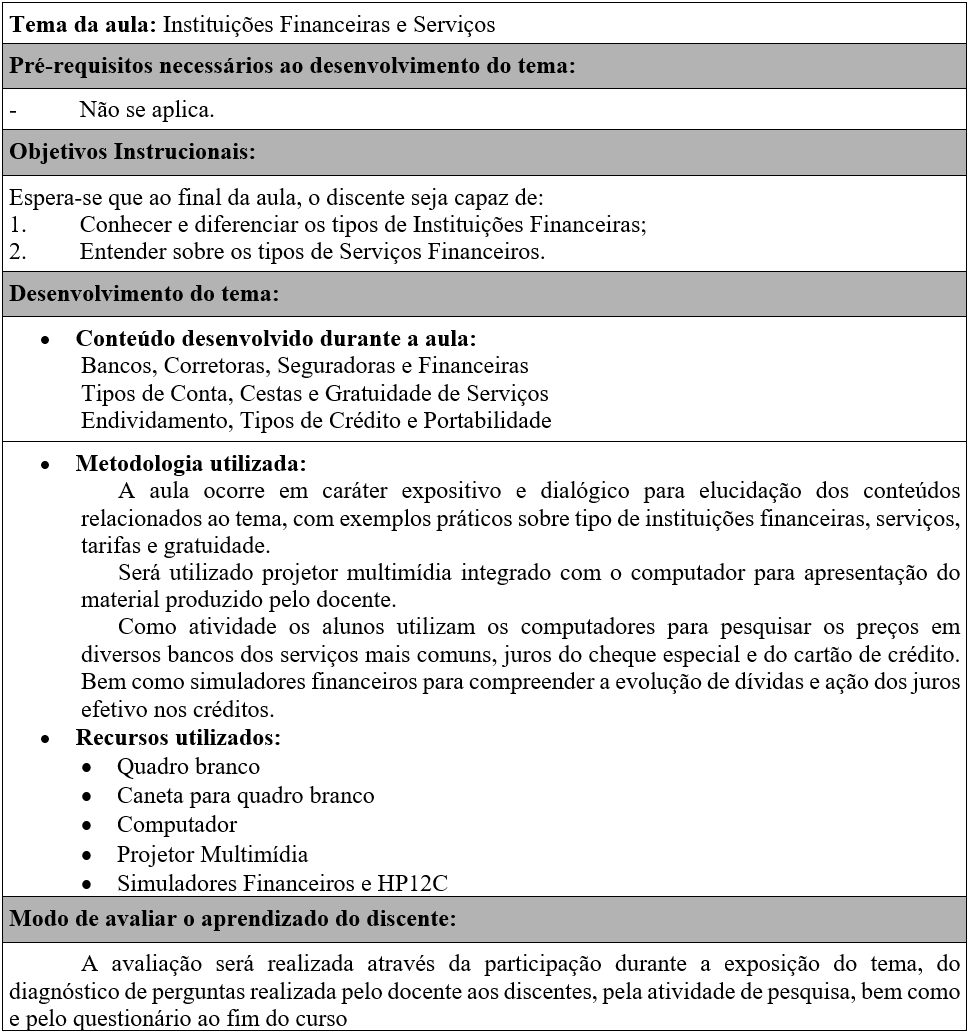
\includegraphics[width=0.9\textwidth]{quadro-10_plano-aula-4}
\legend{\footnotesize Fonte: O autor, 2019}
\label{quad: quadro-10_plano-aula-4}
\end{minipage}
\end{quadro}

Ao final deste encontro aplicando o conhecimento adquirido o aluno alcança o estágio Poupador Concreto desenvolvimento cognitivo financeiro, pois compreende a importância e aplica o planejamento orçamentário, busca sempre poupar recursos, realiza o consumo consciente, conhece os tipos de serviços e instituições financeiros, assim como investe o recurso poupado na caderneta de poupança, por falta de conhecimento em outros investimentos.

\section{5º Encontro - Introdução aos Investimentos}
O objetivo do quinto encontro é demonstrar aos estudantes os aspectos relacionados à introdução de investimentos financeiros, bem como iniciar a transição do desenvolvimento cognitivo financeiro para o último estágio (Investidor Formal). Os conteúdos relacionados a unidade temática estão descritos no quadro \ref{quad: quadro-11_plano-aula-5} que apresenta o plano de aula do 5º encontro.

\graphicspath{{quadros/}} 
\begin{quadro}[!ht]
\centering
\begin{minipage}{1.\textwidth}
\caption{Plano de Aula 5º Encontro do Curso}
\centering
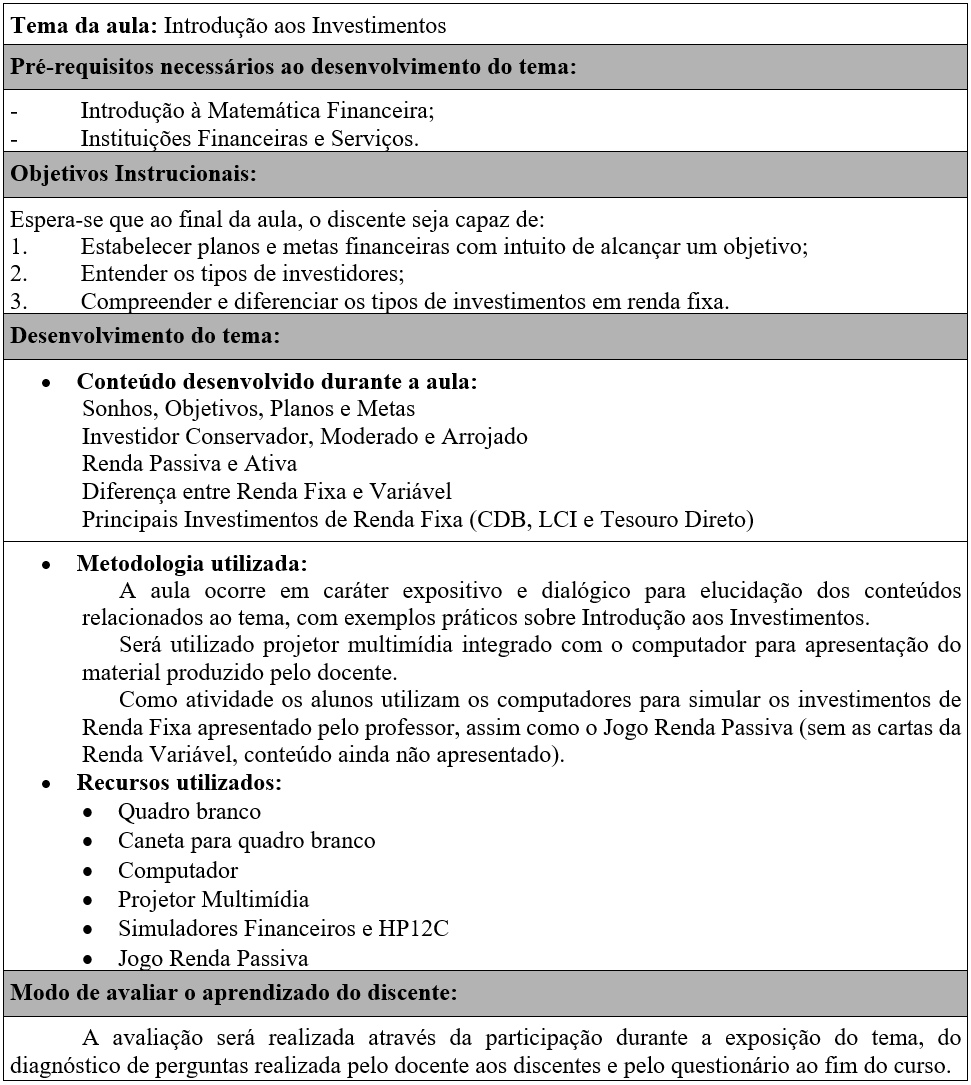
\includegraphics[width=1.0\textwidth]{quadro-11_plano-aula-5}
\legend{\footnotesize Fonte: O autor, 2019}
\label{quad: quadro-11_plano-aula-5}
\end{minipage}
\end{quadro}

Neste encontro ocorre a iniciação do jogo Renda Passiva com explanação de suas cartas, regras, tabuleiro, fichas, pins e jogabilidade, por trata-se de um jogo novo com muitas regras é possível que alguns alunos tenham dificuldades iniciais, entretanto o jogo simula de forma lúdica os conhecimentos adquiridos no curso e do mercado financeiro o que auxilia os alunos na fixação dos conteúdos.

\section{6º Encontro - Revisão com o Jogo Renda Passiva}
O objetivo do sexto encontro é revisar junto com os discentes os conteúdos abordados no curso (Planejamento Orçamentário, Portabilidade de Crédito e Investimentos), bem como a acomodação dos conteúdos estudados através de um jogo sério. O plano de aula deste encontro está descrito no quadro \ref{quad: quadro-12_plano-aula-6}.

\graphicspath{{quadros/}} 
\begin{quadro}[!ht]
\centering
\begin{minipage}{1.\textwidth}
\caption{Plano de Aula 6º Encontro do Curso}
\centering
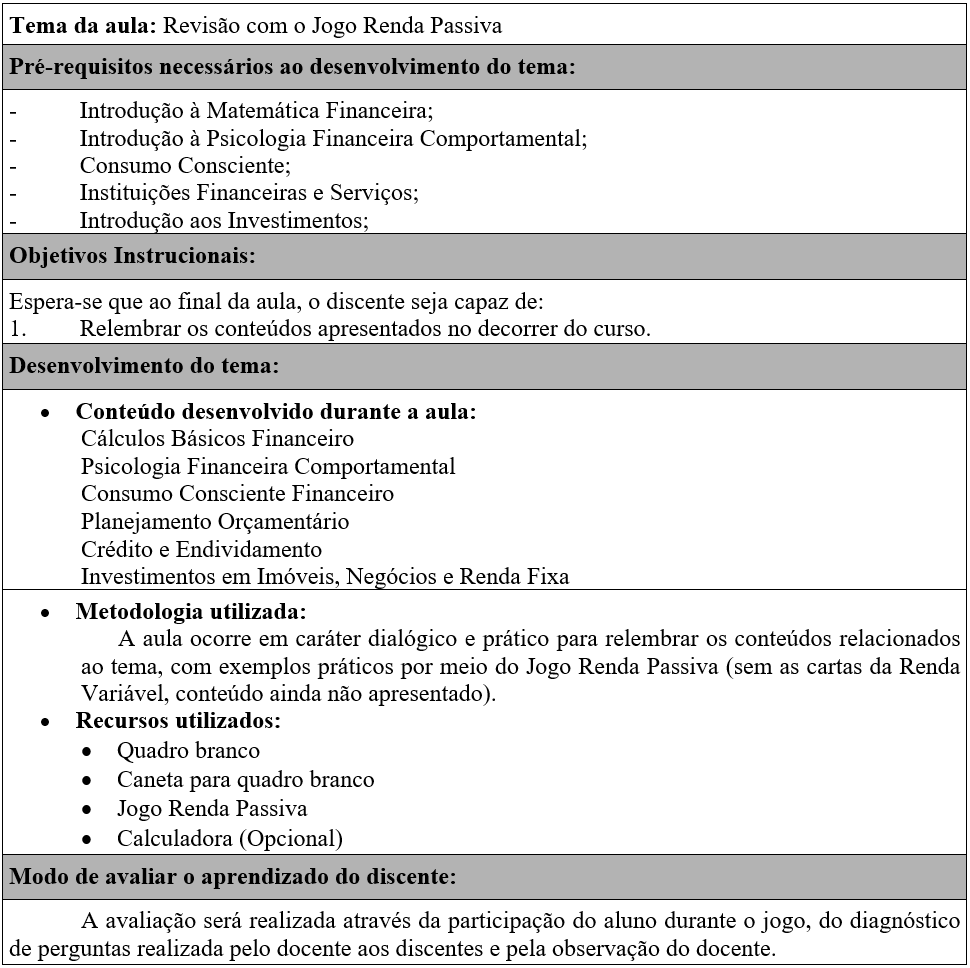
\includegraphics[width=0.9\textwidth]{quadro-12_plano-aula-6}
\legend{\footnotesize Fonte: O autor, 2019}
\label{quad: quadro-12_plano-aula-6}
\end{minipage}
\end{quadro}

\section{7º Encontro - Renda Variável e Previdência}
O objetivo do sétimo encontro é apresentar aos estudantes os aspectos relacionados à introdução de investimentos financeiros especificamente em renda variável, bem como explicar o funcionamento e os tipos de previdência no Brasil. Os conteúdos relacionados a unidade temática estão descritos no quadro \ref{quad: quadro-13_plano-aula-7} que apresenta o plano de aula do 7º encontro.

\graphicspath{{quadros/}} 
\begin{quadro}[!ht]
\centering
\begin{minipage}{1.\textwidth}
\caption{Plano de Aula 7º Encontro do Curso}
\centering
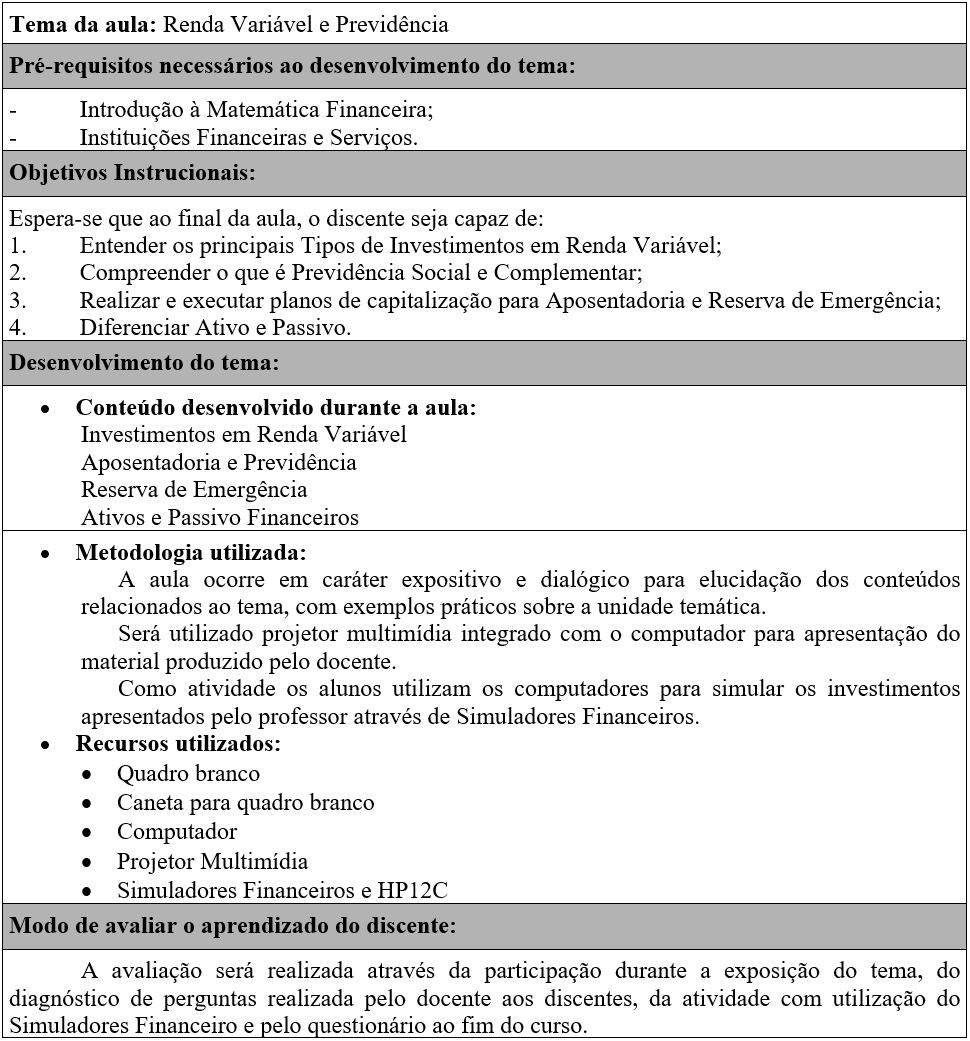
\includegraphics[width=0.9\textwidth]{quadro-13_plano-aula-7}
\legend{\footnotesize Fonte: O autor, 2019}
\label{quad: quadro-13_plano-aula-7}
\end{minipage}
\end{quadro}

Ao final deste encontro aplicando o conhecimento adquirido e buscando estudar novos conteúdos sobre finanças, o aluno poderá alcançar o estágio Investidor Formal do desenvolvimento cognitivo financeiro, pois compreende a importância e aplica o planejamento orçamentário, busca sempre poupar recursos, realiza consumo consciente, conhece os tipos de serviços e instituições financeiras, assim como investe os recursos em diferentes instituições de acordo com o seu perfil e objetivos financeiros.

\section{8º Encontro - Jogo Renda Passiva e Aplicação dos Questionários}
O objetivo do oitavo encontro é revisar junto com os discentes todos os conteúdos abordados no curso através de um jogo sério, entretanto desta vez os alunos utilizam o jogo Renda Passiva com todos os recursos e regras disponíveis. O plano de aula deste encontro está descrito no quadro \ref{quad: quadro-14_plano-aula-8}.

\graphicspath{{quadros/}} 
\begin{quadro}[!ht]
\centering
\begin{minipage}{1.\textwidth}
\caption{Plano de Aula 8º Encontro do Curso}
\centering
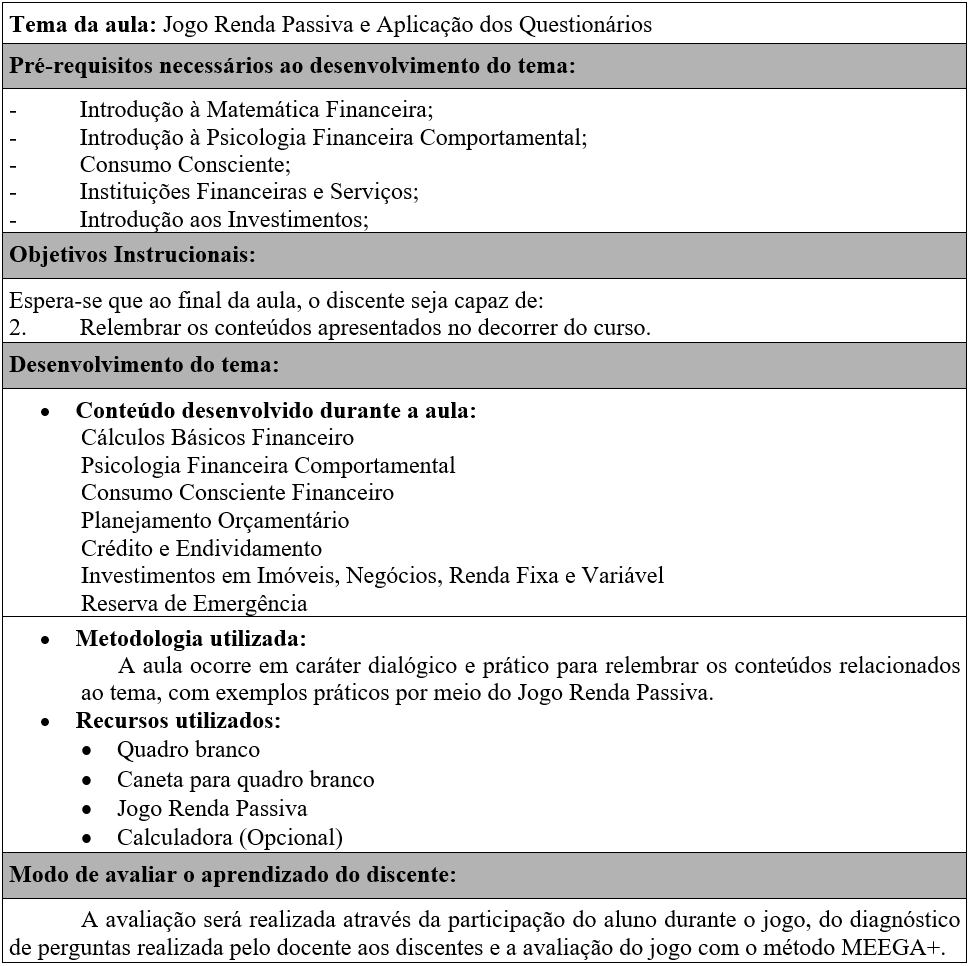
\includegraphics[width=0.9\textwidth]{quadro-14_plano-aula-8}
\legend{\footnotesize Fonte: O autor, 2019}
\label{quad: quadro-14_plano-aula-8}
\end{minipage}
\end{quadro}

Após a utilização do jogo sério é aplicada uma avaliação para compreender experiência do jogador e o processo de aprendizagem utilizando o jogo, por intermédio do método MEEGA+.

Aplicam-se também o Questionário de Avaliação da Aprendizagem (Apêndice \ref{apend-a}) e o Questionário de Avaliação do Curso (Apêndice \ref{apend-b}), para verificar se os objetivos propostos foram alcançados e confirmar ou não a hipótese do presente trabalho.

\chapter{Resultados Parciais}
Este projeto apresentou uma proposta para consolidação da educação financeira para os cursos técnicos da RFEPCT, que possui potencial para ser ampliada para rede pública de ensino, mediado por tecnologias educacionais e o uso de jogos sérios digitais. Procurou apoiar-se em fundamentos teóricos educacionais para possibilitar o seu uso efetivo, visando complementar a formação do estudante brasileiro através de um curso, nesse tema ainda pouco explorado e que impacta diretamente ao longo de sua vida.

O projeto teve alguns resultados surpreendentes e importantes de serem registrados. Embora o curso tenha sido acertado como disciplina não obrigatório e com vaga restrita 19 participantes, despertou interesse de 41 inscritos o que surpreende de forma positiva e revela uma demanda relevante pelo assunto. Essa demanda reprimida levou à necessidade de realizar sorteio para inscrição que, com uma divulgação considerada tímida, mobilizou 15{\%} dos alunos de ensino médio integrado da instituição. Possivelmente, no mundo contemporâneo globalizado e conectado os jovens estudantes estejam mais conscientes sobre a importância da educação financeira, mas ainda lhes faltam ambientes e oportunidades desse aprendizado de forma efetiva.

O conteúdo apresentado no curso de Introdução à Educação Financeira para Jovens do ensino médio integrado disponibilizou aos alunos o conhecimento introdutório sobre finanças, necessário para a alfabetização financeira, abrangendo do primeiro ao último estágio de desenvolvimento do conhecimento financeiro descritos no referencial teórico: Consumidor Sensorial, Consumidor Pré-Poupador, Poupador Concreto e Investidor Formal.

O curso ocorreu de 14/08/2019 a 27/11/2019 com duas aulas semanais. Os alunos do curso tiveram uma frequência superior a 75{\%}, exceto uma aluna que não permaneceu até o final, pois solicitou a transferência para outra instituição, fato que indica o engajamento dos alunos no processo de aprendizagem, tendo em vista que os estudantes não eram obrigados a permanecer no curso, pois este não faz parte do projeto pedagógico do ensino médio da instituição. Por isso, os dados apresentados nos resultados parciais consideram apenas as interações dos 18 alunos com as atividades, tarefas e questionários do curso.

A avaliação do presente projeto baseia-se em 4 instrumentos (Questionário de Avaliação da Aprendizagem, Questionário de Avaliação do Curso e avaliação do resultado da interação com os jogos com o método MEEGA+), entretanto, até o presente momento do projeto, serão descritos os resultados da experiência subjetiva do jogador com o jogo Orçamento Consciente para avaliar seu potencial de aprendizagem, para isto, aplicou-se o questionário do MEEGA+ logo após a interação com os alunos e com o jogo sério. As perguntas do questionário MEEGA+ e os dados coletados com as respostas dos discentes são expostos no Gráfico \ref{graf: grafico-01-meega-orcamento}, bem como os pontos fortes no quadro \ref{quad: quadro-15-pontos-fortes-orçamento-consciente}, sugestões de melhoria no quadro \ref{quad: quadro-16-melhoria-orçamento-consciente} e comentários adicionais no quadro \ref{quad: quadro-17-comentario-orçamento-consciente}.

\graphicspath{{graficos/}} 
\begin{grafico}[!ht]
\centering
%\begin{minipage}{1.\textwidth}
\caption{(MEEGA+) Avaliação do Jogo Orçamento Consciente}
\centering
\includegraphics[width=1.0\textwidth]{Grafico1 - Orçamento Consciente}
\legend{\footnotesize Fonte: Dos autores. Adaptado de Petri (\citeyear{petri2017})}
\label{graf: grafico-01-meega-orcamento}
%\end{minipage}
\end{grafico}

Os resultados acerca da experiência do jogador revelam que os aspectos necessários para melhoria do jogo estão relacionados ao “Desafio”, “Interação social” e à “Atenção focada” (concentração de cores laranja e amarelo do Gráfico \ref{graf: grafico-01-meega-orcamento}), abrindo margem para a hipótese de que a falta de incentivo à interação entre os jogadores, bem como de uma progressão de desafios mais adequada pode ter influenciado no engajamento por parte dos alunos. Uma possível interpretação destes resultados pode sugerir que a atenção dos jogadores reduziu à medida que aprenderam a utilizar da forma lenta de pensar para cumprir com os objetivos, tornando o restante do jogo pouco desafiador para alguns.

\graphicspath{{quadros/}} 
\begin{quadro}[!ht]
\centering
\begin{minipage}{1.\textwidth}
\caption{Jogo Orçamento Consciente (Pontos Fortes)}
\centering
\includegraphics[width=1.0\textwidth]{quadro-15-pontos-fortes-orçamento-consciente}
\legend{\footnotesize Fonte: O autor, 2019}
\label{quad: quadro-15-pontos-fortes-orçamento-consciente}
\end{minipage}
\end{quadro}  

Na seção de pontos fortes do questionário MEEGA+, nota-se relatos acerca do pensamento rápido, gatilhos mentais, comportamento financeiro e compreensão da disciplina como pontos fortes do jogo. Os relatos dos alunos no quadro \ref{quad: quadro-15-pontos-fortes-orçamento-consciente} e na “Percepção de Aprendizagem” (Gráfico \ref{graf: grafico-01-meega-orcamento}) confirma a hipótese que a utilização deste jogo sério facilitou o processo de aprendizagem e satisfação dos discentes, e também, sugerem que a ideia dos desenvolvedores do jogo foi adequadamente expressa e percebida pelos jogadores. Tendo em vista que a ideia norteadora durante o desenvolvimento do projeto foi produzir um ambiente no qual o jogador precisasse lidar com sua forma rápida de pensar e passasse a pensar de forma lenta a fim de se obter mais recompensas, o jogo alcançou o objetivo proposto pelos desenvolvedores, pois, favoreceu a aprendizagem dos alunos de forma lúdica.

Na seção de sugestões de melhorias do questionário MEEGA+ (quadro \ref{quad: quadro-16-melhoria-orçamento-consciente}), os relatos dos alunos apontam, principalmente, a ampliação do jogo para que este possa disponibilizar informações e sugestões de planejamento financeiro, recompensas maiores por aplicar um bom planejamento, adicionar mais opções de produtos e adicionar outros elementos ao jogo, também sugeriram melhorar o designer e aumento no tempo para compras. Dois estudantes apontaram nesta seção uma percepção que o jogo disponibiliza poucos produtos relacionados à saúde, circunstância colocada propositalmente pelos desenvolvedores, pois, no desenvolvimento do jogo procurou-se refletir o orçamento financeiro no qual o gasto com alimentação e compras é maior do que os gastos com saúde.

\graphicspath{{quadros/}} 
\begin{quadro}[!ht]
\centering
\begin{minipage}{1.\textwidth}
\caption{Jogo Orçamento Consciente (Sugestão de Melhorias)}
\centering
\includegraphics[width=1.0\textwidth]{quadro-16-melhoria-orçamento-consciente}
\legend{\footnotesize Fonte: O autor, 2019}
\label{quad: quadro-16-melhoria-orçamento-consciente}
\end{minipage}
\end{quadro}

\newpage
Quanto aos comentários adicionais do questionário MEEGA+ (quadro \ref{quad: quadro-17-comentario-orçamento-consciente}), apenas 6 alunos responderam esta seção, na maior parte das respostas os alunos elogiaram o jogo e o curso, somente um aluno indicou uma melhoria, também no sentido de ampliação para que o jogo forneça direcionamento ao jogador.

\graphicspath{{quadros/}} 
\begin{quadro}[!ht]
\centering
\begin{minipage}{1.\textwidth}
\caption{Jogo Orçamento Consciente (Comentários Adicionais)}
\centering
\includegraphics[width=0.5\textwidth]{quadro-17-comentario-orçamento-consciente}
\legend{\footnotesize Fonte: O autor, 2019}
\label{quad: quadro-17-comentario-orçamento-consciente}
\end{minipage}
\end{quadro}

Por intermédio dos relatos nos pontos fortes, sugestões de melhoria e comentários adicionais, observa-se que o jogo foi bem recebido pelos alunos no processo de aprendizagem, apesar de tratar-se apenas de um protótipo passível das melhorias sugestionadas pelos participantes da pesquisa, sugestões que poderão proporcionar maior qualidade ao jogo e, consequentemente, ao processo de aprendizagem dos estudantes.

Em relação à elaboração do presente trabalho considera-se que a realização foi parcial pelo fato de que a análise dos dados obtidos não está finalizada. Por isso, pretende-se nos próximos meses investigar as respostas dos alunos acerca da experiência da interação com jogo renda passiva, obtida pelo questionário do MEEGA+, assim como apurar a retenção dos alunos sobre os principais temas abordados no curso, através dos dados adquiridos pelo Questionário de Avaliação da Aprendizagem (Apêndice \ref{apend-a}), e averiguar a percepção e impacto do curso nos alunos, por meio das respostas alcançadas no Questionário de Avaliação do Curso (Apêndice \ref{apend-b}). Por último, discorrer sobre os resultados encontrados na investigação dos dados levantados, no intuito de verificar se os objetivos foram alcançados e a confirmação ou não da hipótese deste trabalho.

Espera-se que os resultados deste trabalho possa impactar no processo de ensino-aprendizagem da educação financeira no ensino médio da RFEPCT e de outras redes de ensino, bem como, que o curso possa ser usado amplamente por instituições de ensino brasileiras, evoluindo-o e integrando-o definitivamente aos currículos do ensino médio, contribuindo efetivamente na alfabetização financeira dos estudantes. Almeja-se também com este trabalho, colaborar para a formação sólida e ampla dos estudantes profissionais, para que possam enfrentar os desafios impostos pela sociedade atual, que exige dos cidadãos mais conhecimento sobre economia e finanças.

% ==============================================
% ELEMENTOS PÓS-TEXTUAIS
% ==============================================
\postextual
% ||||||||||||||||||||||||||||||||||||||||||||||
% REFERÊNCIAS BIBLIOGRÁFICAS
% ||||||||||||||||||||||||||||||||||||||||||||||
%\bibliography{bibfile2}
% bibliografia john
\bibliography{ref-bibliografica}
% ----------------------------------------------
% Glossário
% ----------------------------------------------
% Consulte o manual da classe abntex2 para orientações sobre o glossário.
%
%\glossary
% ||||||||||||||||||||||||||||||||||||||||||||||
% APÊNDICES
% ||||||||||||||||||||||||||||||||||||||||||||||
% Imprime uma página indicando o início dos apêndices
%\partapendices
% ----------------------------------------------
% Apêndice
% ----------------------------------------------
\begin{apendicesenv}
    \chapter{Avaliação da Aprendizagem}\label{apend-a}
    \begin{enumerate}
    \item O que é a educação financeira?
    
    \item Qual as características de um bom orçamento financeiro?
    
    \item Considerando a Educação Financeira e a Matemática Financeira assinale a alternativa correta:
        \begin{enumerate}
            \item  (   ) A Educação Financeira promove reflexão sobre a vida financeira.
           \item   (   ) A Matemática Financeira trata sobre hábitos financeiros.
            \item  (   ) A Matemática Financeira aborda os tipos de investimentos.
            \item  (   ) A Educação Financeira e a Matemática Financeira são sinônimos.
        \end{enumerate}
    
    \item Selecione a alternativa correta. O orçamento pessoal ou familiar auxilia:
        \begin{enumerate} 
            \item (   ) No controle de receitas e despesas
            \item (   ) Administrar os recursos financeiros de forma consciente
            \item (   ) No controle das dívidas
            \item (   ) Todas as alternativas anteriores
        \end{enumerate}
        
    \item Abaixo há uma lista de itens relacionados às necessidades, desejos e desperdício. Assinale as alternativas referentes somente às necessidades, pode-se escolher mais de uma alternativa.
        \begin{enumerate}
            \item (   ) Sapato de marca - Cirurgia plástica
            \item (   ) Passagem de ônibus - Remédio
            \item (   ) Restaurantes - Viagens - Carro do ano
            \item (   ) Aluguel da casa - Roupas - Lazer
        \end{enumerate}
    
    \item Escolha a alternativa abaixo que representa a ordem das etapas de um Orçamento Financeiro.
        \begin{enumerate}
            \item (   ) Avaliar, Agrupar, Planejar e Registrar
            \item (   ) Registrar, Planejar, Avaliar, Agrupar
            \item (   ) Planejar, Registrar, Agrupar e Avaliar
            \item (   ) Registrar, Agrupar, Planejar e Avaliar
        \end{enumerate}
    
    \newpage    
    \item Qual o tipo de juros é utilizado para rentabilidade dos investimentos?
        \begin{enumerate}
            \item (   ) Juros Simples
            \item (   ) Juros de Mora
            \item (   ) Juros Compostos
            \item (   ) Juros de Capital Próprio
        \end{enumerate}
        
    \item Considerando que a inflação é a variação mensal dos preços, marque a alternativa que representa o índice oficial que o governo brasileiro utiliza para medir a inflação nacional.
        \begin{enumerate}
            \item (   ) CDI
            \item (   ) SELIC
            \item (   ) CDB
            \item (   ) IPCA
        \end{enumerate}
        
    \item Investimento é aplicação do dinheiro poupado para obtenção de juros ou dividendos. Eles possuem três característica Risco, Rentabilidade e Liquidez. Sabendo disso assinale a alternativa que corresponde a definição de Liquidez.
        \begin{enumerate}
            \item (   ) É a probabilidade de ocorrer perdas no investimento
            \item (   ) É a possibilidade do investimento ser transformado em dinheiro
            \item (   ) É a remuneração recebida pelo investimento
        \end{enumerate}
        
    \item Assinale a alternativa cujo investimento não é garantido pelo FGC.
        \begin{enumerate}
            \item (   ) Tesouro Direto
            \item (   ) LCI/LCA
            \item (   ) CDB
            \item (   ) Poupança
        \end{enumerate}
        
    \item Assinale a características de um Investimento em Renda Variável.
        \begin{enumerate}
            \item (   ) Esse tipo de investimento não possui riscos 
            \item (   ) A rentabilidade desse investimento é garantida
            \item (   ) Esse tipo de investimento possui riscos
            \item (   ) É coberto pelo Fundo Garantidor de Crédito
        \end{enumerate}
\end{enumerate}

    
    \chapter{Avaliação do Curso}\label{apend-b}
    \begin{enumerate}
    \item O que te motivou a participar deste curso?
    
    \item Você conhecia os temas abordados nas aulas antes do curso? Se sim, quais temas?
    
    \item Você considera os temas abordados nas aulas importantes para o seu futuro?
    
    \item Os simuladores, jogos (físicos e digitais) e os ambientes virtuais auxiliaram na compreensão dos assuntos abordados durante as aulas? Caso sim de qual forma?
    
    \item Você tem interesse em buscar de novos conhecimentos sobre os temas abordados nas aulas?
    
    \item Você conversou com sua família ou amigos ou parentes sobre o curso? Se sim com quem e quais temas?
    
    \item Quais os temas do curso que mais gostou?
    
    \item O curso está atendendo as suas expectativas.
        \begin{enumerate}
            \item Concordo Totalmente
            \item Concordo Parcialmente
            \item Indiferente
            \item Discordo Parcialmente
            \item Discordo Totalmente
        \end{enumerate}
    
    \item Há alguma sugestão de melhoria, elogio e/ou crítica que gostaria de fazer em relação ao curso?
\end{enumerate}
    
    \chapter{Aplicação do Conhecimento}\label{apend-c}
    Em relação à sua vida financeira atual responda às seguintes perguntas:
\begin{enumerate}
   \item Quais as fontes de dinheiro você utiliza para comprar produtos ou serviços? (Ex: trabalho, estágio, bolsa de estudo, auxílio escolar, mesada, dinheiro dado pelos responsáveis quando necessita, pensão etc).
   
   \item A sua participação no curso de Educação Financeira proporcionou quais mudanças em sua vida e de sua família?
   
   \item De que forma o conhecimento adquirido no curso está auxiliando você e sua família a enfrentar os problemas financeiros causado pela pandemia do COVID-19?
   
   \item Como normalmente você realiza a compra de produtos e serviços?
        \begin{enumerate}
            \item Compro por impulso quando tenho dinheiro para comprar à vista
            \item Compro por impulso e parcelo no cartão de crédito
            \item Planejo, pesquiso e economizo dinheiro antes de comprar à vista
            \item Planejo, pesquiso antes de comprar parcelado no cartão
            \item Outros:
        \end{enumerate}
        
    \item Como você controla suas receitas e gastos mensais?
        \begin{enumerate}
            \item Não anoto nenhum gasto ou receita mensal
            \item Registro todos os gastos e receitas que possuo
            \item Registro apenas gastos e receitas grandes
            \item Outros:
        \end{enumerate}
        
    \item Você separa parte do dinheiro recebido para investir?
        \begin{enumerate}
            \item Sim, antes de gastar
            \item Sim, se sobrar
            \item Não, sempre utilizo todo dinheiro que ganho
            \item Outros:
        \end{enumerate}
    
    \item Normalmente em qual tipo de investimento você aplica o dinheiro poupado? (É possível marcar mais de uma opção).
        \begin{enumerate}
            \item Não poupo dinheiro para aplicar
            \item Caderneta de poupança
            \item Outros investimentos de renda fixa
            \item Investimentos de renda variável
            \item Outros:
        \end{enumerate}
        
    \item Você planeja e economiza parte do dinheiro recebido para sonhos e objetivos futuros?
        \begin{enumerate}
            \item Não, vivo apenas o presente
            \item Não, pois nunca sobra dinheiro
            \item Sim, tenho metas, poupo e aplico dinheiro para objetivos futuros
            \item Outros:
        \end{enumerate}
\end{enumerate}
    
    \chapter{APLICAÇÃO DO CONHECIMENTO - RESPOSTAS}\label{apend-d}
    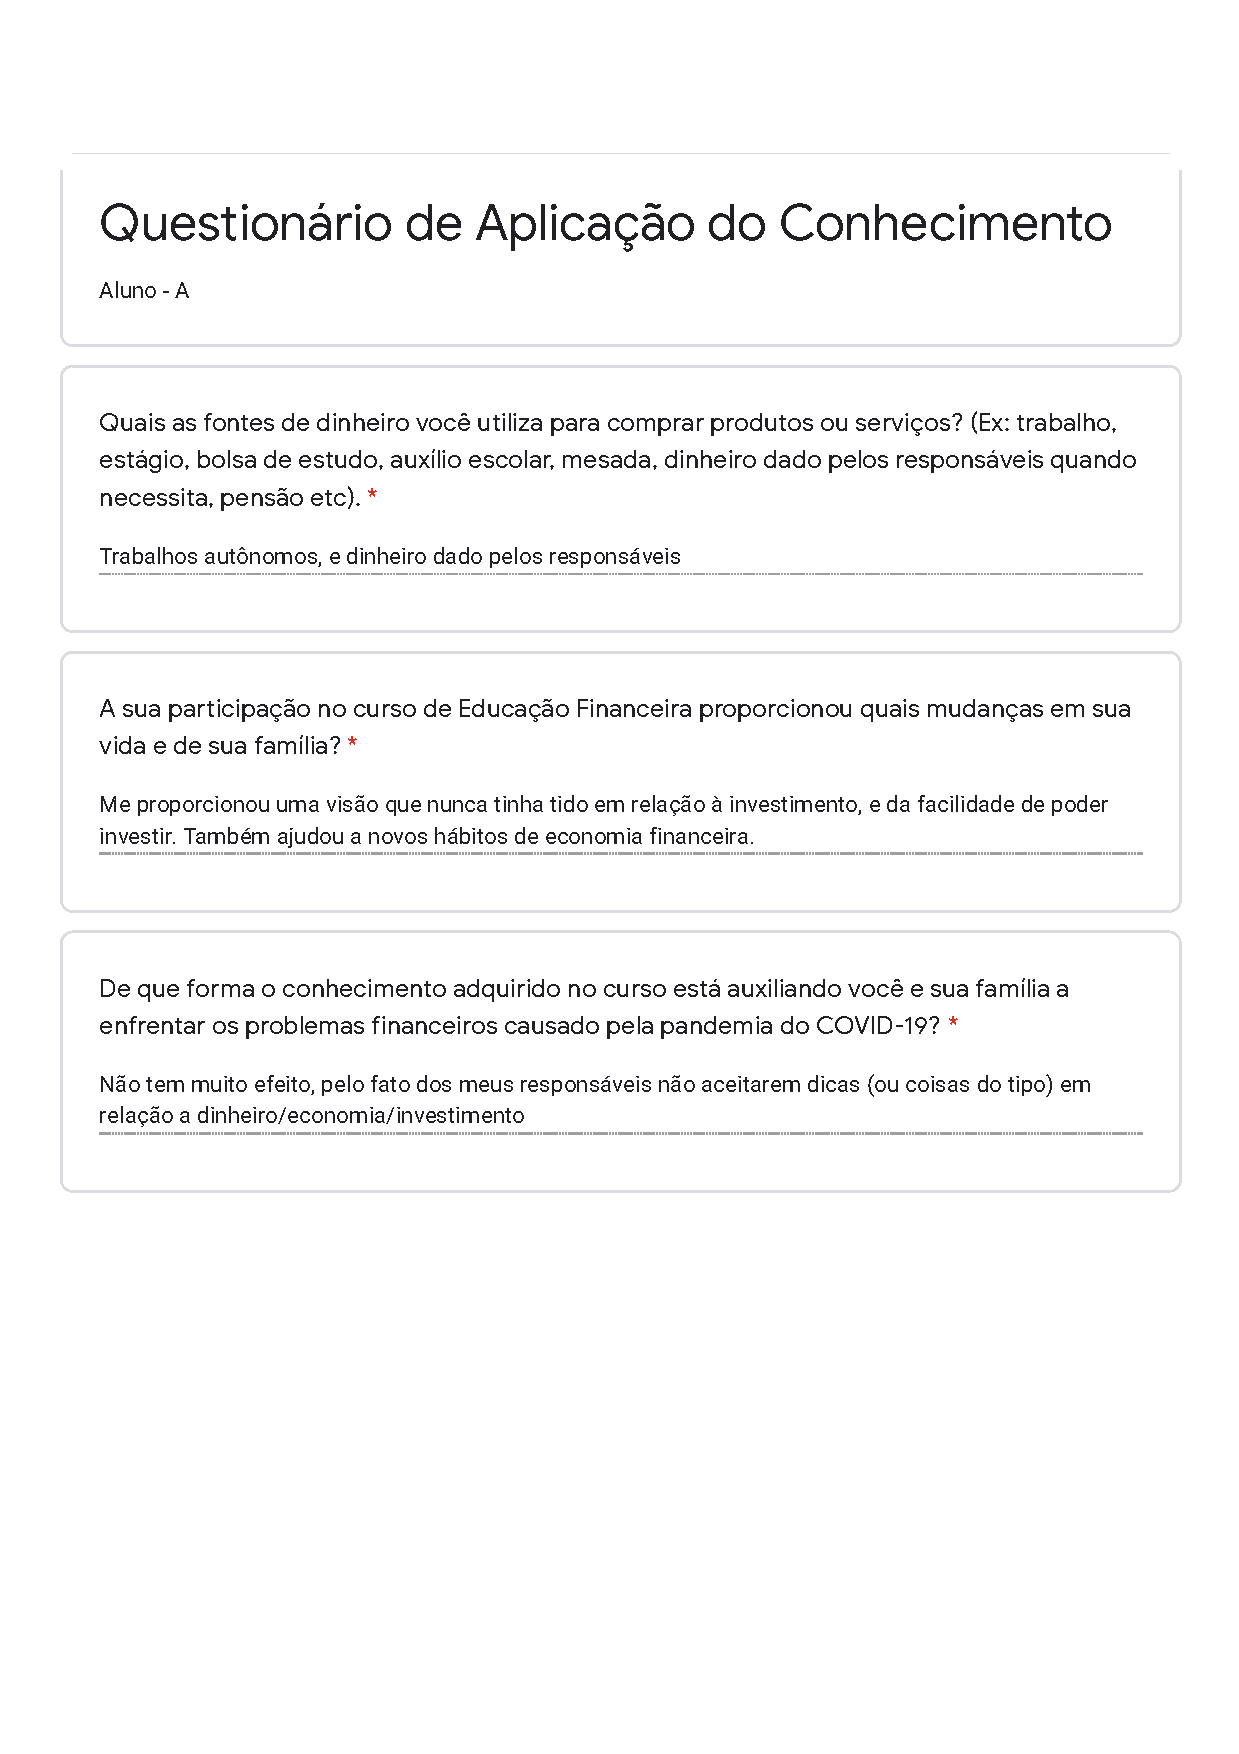
\includepdf[pages=-]{apendices/aplicacao-conhecimento-resposta.pdf}
    
%\includepdf[pages=-]{apendices/apendice.pdf}

\end{apendicesenv}

% ||||||||||||||||||||||||||||||||||||||||||||||
% ANEXOS
% ||||||||||||||||||||||||||||||||||||||||||||||
%\begin{anexosenv}
% Imprime uma página indicando o início dos anexos
%\partanexos
% ----------------------------------------------
% Anexo 1
% ----------------------------------------------
%\chapter{Datasheet}\label{anexo1}
%\includepdf[pages=-]{pdfs/Datasheet.pdf}
% ----------------------------------------------
% Anexo 2
% ----------------------------------------------
%\chapter{Anexo 2}
%\end{anexosenv}
% ==============================================
% INDICE REMISSIVO
% ==============================================
\phantompart
\printindex
% ----------------------------------------------
% ||||||||||||||||||||||||||||||||||||||||||||||
% DOCUMENTO PARA ENTREGA VERSÃO FINAL
%||||||||||||||||||||||||||||||||||||||||||||||
\begin{comment}

\clearpage\thispagestyle{empty}\addtocounter{page}{-1}
\section*{ENTREGA DA VERSÃO FINAL DE DISSERTAÇÃO}

\vspace*{2cm}
Eu, \textsc{\imprimirorientador}, autorizo o aluno(a) \textsc{\imprimirautor} a entregar a versão final da dissertação de mestrado, à secretaria do MPIE, que foi por mim analisada e está de acordo com os apontamentos feitos pelos membros da banca de apresentação do referido aluno.

\vspace*{1cm}
\begin{center}   
   \assinatura{{\imprimirorientador} \\ Orientador}
\end{center}

\vspace*{1cm}
\begin{flushright}
	\imprimirlocal, 11 de Julho de \imprimirdata.
\end{flushright}
\clearpage
\end{comment}

\end{document}